%% ----------------------------------------------------------------
%% Thesis.tex -- MAIN FILE (the one that you compile with LaTeX)
%% ----------------------------------------------------------------

% Set up the document
\documentclass[a4paper, 11pt, oneside]{Thesis}  % Use the "Thesis" style, based on the ECS Thesis style by Steve Gunn
\graphicspath{Figures/}  % Location of the graphics files (set up for graphics to be in PDF format)


\usepackage[table,xcdraw]{xcolor}

% Include any extra LaTeX packages required
\usepackage[square, numbers, comma, sort&compress, authoryear]{natbib}  % Use the "Natbib" style for the references in the Bibliography
\usepackage{verbatim}  % Needed for the "comment" environment to make LaTeX comments
\usepackage{vector}  % Allows "\bvec{}" and "\buvec{}" for "blackboard" style bold vectors in maths
\hypersetup{urlcolor=blue, colorlinks=true}  % Colours hyperlinks in blue, but this can be distracting if there are many links.

\newcommand{\fig}[1]{Figure~\ref{fig:#1}}
\newcommand{\sect}[1]{Section~\ref{sect:#1}}
\newcommand{\chapt}[1]{Chapter~\ref{chapt:#1}}
\newcommand{\tab}[1]{Table~\ref{tab:#1}}
\newcommand{\alg}[1]{Algorithm~\ref{alg:#1}}
\newcommand{\eq}[1]{(\ref{eq:#1})}

\usepackage{verbatimbox}
\usepackage{todonotes}
\usepackage{gensymb}
\usepackage{enumitem}



%%%% bilinear
\usepackage{times}

\usepackage{graphicx}
\usepackage{amsmath}
\usepackage{amssymb}
\usepackage{wrapfig}
\usepackage{placeins}
%\usepackage{authblk}
\usepackage{tabularx} 
\usepackage{fancyhdr}



\renewcommand{\headrulewidth}{0pt}


\newcommand{\p}{\mathcal{P}}
\newcommand{\e}{e}
\newcommand{\E}{E}
\newcommand\cincludegraphics[2][]{\raisebox{-0.45\height}{\includegraphics[#1]{#2}}}

\newcommand{\Sp}{{\mathcal S}^{+}}
\newcommand{\Sgen}{{\mathcal S}}
\newcommand{\Sm}{{\mathcal S}^{-}}
\newcommand{\spr}[2]{{\langle{}#1,#2\rangle}}
\newcommand{\prp}{p^{+}}
\newcommand{\prm}{p^{-}}
\newcommand{\Hp}{H^{+}}
\newcommand{\Hm}{H^{-}}
\newcommand{\hp}{h^{+}}
\newcommand{\hm}{h^{-}}


%%%%
%\newcommand{\todo}[1][]{\@latex@warning{TODO #1}\fbox{TODO\dots}}

%\usepackage{graphicx}
%\usepackage{amsmath,amssymb} % define this before the line numbering.
%\usepackage{placeins}
%\usepackage{color}
%\usepackage[width=122mm,left=12mm,paperwidth=146mm,height=193mm,top=12mm,paperheight=217mm]{geometry}
%\usepackage{subfigure}
%\usepackage{xr-hyper}
%\usepackage[colorlinks=true]{hyperref}
%\usepackage{textcomp}

% Tikz-related stuff.
\usepackage{tikz}
\usetikzlibrary{arrows.meta}
\usetikzlibrary{backgrounds}
\usetikzlibrary{calc}
\usetikzlibrary{decorations.markings}
\usetikzlibrary{decorations.text}
\usetikzlibrary{fit}
\usetikzlibrary{positioning}
\usetikzlibrary{shapes.geometric}
\usetikzlibrary{3d}

% PGF-plots-related stuff.
\usepackage{pgfplots}
\pgfplotsset{compat=newest}
\newlength\figureheight
\newlength\figurewidth
% \usepgfplotslibrary{external}
% \tikzexternalize


\def\mystrut{\rule[-.3\baselineskip]{0pt}{0.5\baselineskip}}

\input{colors}

%% ----------------------------------------------------------------
\begin{document}
\frontmatter      % Begin Roman style (i, ii, iii, iv...) page numbering

% Set up the Title Page
\title  {Human re-identification and recognition using deep learning methods.}
\authors  {\texorpdfstring
            {\href{evgeniya.ustinova@skoltech.ru}{Evgeniya Ustinova}}
            {Evgeniya Ustinova}
            }
\addresses  {\groupname\\\deptname\\\univname}  % Do not change this here, instead these must be set in the "Thesis.cls" file, please look through it instead
\date       {\today}
\subject    {}
\keywords   {}

\maketitle
%% ----------------------------------------------------------------

\setstretch{1.3}  % It is better to have smaller font and larger line spacing than the other way round

% Define the page headers using the FancyHdr package and set up for one-sided printing
\fancyhead{}  % Clears all page headers and footers
\rhead{\thepage}  % Sets the right side header to show the page number
\lhead{}  % Clears the left side page header

\pagestyle{fancy}  % Finally, use the "fancy" page style to implement the FancyHdr headers

%% ----------------------------------------------------------------
% Declaration Page required for the Thesis, your institution may give you a different text to place here
%\Declaration{

%\addtocontents{toc}{\vspace{1em}}  % Add a gap in the Contents, for aesthetics

%I, AUTHOR NAME, declare that this thesis titled, `THESIS TITLE' and the work presented in it are my own. I confirm that:

%\begin{itemize}
%\item[\tiny{$\blacksquare$}] This work was done wholly or mainly while in candidature for a research degree at this University.

%\item[\tiny{$\blacksquare$}] Where any part of this thesis has previously been submitted for a degree or any other qualification at this University or any other institution, this has been clearly stated.

%\item[\tiny{$\blacksquare$}] Where I have consulted the published work of others, this is always clearly attributed.

%\item[\tiny{$\blacksquare$}] Where I have quoted from the work of others, the source is always given. With the exception of such quotations, this thesis is entirely my own work.

%\item[\tiny{$\blacksquare$}] I have acknowledged all main sources of help.

%\item[\tiny{$\blacksquare$}] Where the thesis is based on work done by myself jointly with others, I have made clear exactly what was done by others and what I have contributed myself.
%\\
%\end{itemize}


%Signed:\\
%\rule[1em]{25em}{0.5pt}  % This prints a line for the signature

%Date:\\
%\rule[1em]{25em}{0.5pt}  % This prints a line to write the date
%}
%\clearpage  % Declaration ended, now start a new page

%% ----------------------------------------------------------------
% The "Funny Quote Page"
%\pagestyle{empty}  % No headers or footers for the following pages

%\null\vfill
% Now comes the "Funny Quote", written in italics
%\textit{``You're just too good to be true \\
%Can't take my eyes off you.''}

%\begin{flushright}
%Bob Crewe, Bob Gaudio
%\end{flushright}

%\vfill\vfill\vfill\vfill\vfill\vfill\null
%\clearpage  % Funny Quote page ended, start a new page
%% ----------------------------------------------------------------

% The Abstract Page
\addtotoc{Abstract}  % Add the "Abstract" page entry to the Contents
\abstract{
\addtocontents{toc}{\vspace{1em}}  % Add a gap in the Contents, for aesthetics


In this work, I study and develop methods for estimating similarity of human images. The task is to measure image correspondence in such a way that the estimated similarity would be high for images of the same class and low for images of the different classes, where the classes may be defined in different ways depending on the given problem.

Two specific problems are approached in this work. The first one is the person re-identification (person re-id) problem where the domain is pedestrian images captured by surveillance cameras. %The second one is face super-resolution aimed to improve the recognition quality. 
}

\clearpage  % Abstract ended, start a new page
%% ----------------------------------------------------------------

\setstretch{1.3}  % Reset the line-spacing to 1.3 for body text (if it has changed)

% The Acknowledgements page, for thanking everyone
%\acknowledgements{
%\addtocontents{toc}{\vspace{1em}}  % Add a gap in the Contents, for aesthetics

%The acknowledgements and the people to thank go here, don't forget to include your project advisor\ldots

%}
%\clearpage  % End of the Acknowledgements
%% ----------------------------------------------------------------

\pagestyle{fancy}  %The page style headers have been "empty" all this time, now use the "fancy" headers as defined before to bring them back


%% ----------------------------------------------------------------
%\lhead{\emph{Contents}}  % Set the left side page header to "Contents"
\tableofcontents  % Write out the Table of Contents

%% ----------------------------------------------------------------
%\lhead{\emph{List of Figures}}  % Set the left side page header to "List if Figures"
\listoffigures  % Write out the List of Figures

%% ----------------------------------------------------------------
%\lhead{\emph{List of Tables}}  % Set the left side page header to "List of Tables"
\listoftables  % Write out the List of Tables

%% ----------------------------------------------------------------
\setstretch{1.5}  % Set the line spacing to 1.5, this makes the following tables easier to read

%\clearpage  % Start a new page
%\lhead{\emph{Abbreviations}}  % Set the left side page header to "Abbreviations"
%\listofsymbols{ll}  % Include a list of Abbreviations (a table of two columns)
%{
% \textbf{Acronym} & \textbf{W}hat (it) \textbf{S}tands \textbf{F}or \\
%\textbf{LAH} & \textbf{L}ist \textbf{A}bbreviations \textbf{H}ere \\
%
%}

%% ----------------------------------------------------------------
%\clearpage  % Start a new page
%\lhead{\emph{Physical Constants}}  % Set the left side page header to "Physical Constants"
%\listofconstants{lrcl}  % Include a list of Physical Constants (a four column table)
%{
% Constant Name & Symbol & = & Constant Value (with units) \\
%Speed of Light & $c$ & $=$ & $2.997\ 924\ 58\times10^{8}\ \mbox{ms}^{-\mbox{s}}$ (exact)\\

%}

%% ----------------------------------------------------------------
%\clearpage  %Start a new page
%\lhead{\emph{Symbols}}  % Set the left side page header to "Symbols"
%\listofnomenclature{lll}  % Include a list of Symbols (a three column table)
%{
% symbol & name & unit \\
%$a$ & distance & m \\
%$P$ & power & W (Js$^{-1}$) \\
%& & \\ % Gap to separate the Roman symbols from the Greek
%$\omega$ & angular frequency & rads$^{-1}$ \\
%}
%% ----------------------------------------------------------------
% End of the pre-able, contents and lists of things
% Begin the Dedication page

\setstretch{1.3}  % Return the line spacing back to 1.3

%\pagestyle{empty}  % Page style needs to be empty for this page
%\dedicatory{For/Dedicated to/To my\ldots}

\addtocontents{toc}{\vspace{2em}}  % Add a gap in the Contents, for aesthetics


%% ----------------------------------------------------------------
\mainmatter	  % Begin normal, numeric (1,2,3...) page numbering
\pagestyle{fancy}  % Return the page headers back to the "fancy" style

% Include the chapters of the thesis, as separate files
% Just uncomment the lines as you write the chapters


\newcommand{\histroot}{Chapters/histloss}

\chapter{Learning Deep Embeddings with Histogram Loss}
\label{chapt:hist}
 


%todo something about the importance of the loss function compared to architecture from israel paper?
\section{Motivation}
%: objective functions for similarity learning

% The problem of learning deep embeddings is considered in this chapter. Usually, such learning is performed using siamese architectures described in  \sect{intro_siamese} to solve the similarity estimation \pr{similarity_estimation}. Under this approach, complex input patterns (\eg{} images) are mapped into a high-dimensional space through a chain of feed-forward transformations, while the parameters of the transformations are learned from a large amount of supervised data. The \textit{objective} of the learning process is to achieve the proximity of semantically related patterns (\eg{} images of the same person) and avoid the proximity of semantically unrelated (\eg{} images of different people) in the target space. It should be noted that this work is focused on simple similarity measures such as Euclidean distance or scalar products, as they allow fast evaluation.

% The formulation of an objective function for learning embeddings depends on the exact formulation of \pr{similarity_estimation}. It can be formalized in several different ways depending on the setting: 
% \begin{enumerate}
% \item \label{assumption_1} whether we need all the positive pairs to have higher similarity values than \textit{all} the negative pairs,

% \item \label{assumption_2} or we only need this condition fulfilled for each separate identity. 
% \end{enumerate}

In more detail, the latter means that positive pairs ${(x_i^a, x_j^a)}_{i,j}$ that consist of images of some identity $a$ should have the higher similarity value compared only to corresponding negative pairs ${(x_i^a, x_k^{n})}_{i,k}$, that contain one image for the identity $a$ and the second image - for some other identity $n$. 

According to one of the two described assumptions, the training data for the similarity-learning tasks may be formed in one of the following basic ways:

\begin{itemize}
    \item a set of positive pairs and a set of negative pairs:
        \begin{equation}
          \begin{aligned}
          \label{c:pairs_constraints}
                   S = \{(x_i^a, x_j^a): x_i^a \text{ and }& x_j^a \text{ are similar}\}, & \\
                   D = \{(x_i^b, x_j^c): x_i^b \text{ and }& x_j^c \text{ are not similar}\};&\\
          \end{aligned}
        \end{equation}

     
    \item a set of triplets:
     \begin{equation}
     \label{c:triplets_constraints}
          R = \{(x_i^a, x_j^a, x_k^n): x_i^a \text{ is more similar to } x_j^p \text{ than to } x_k^n\}; 
     \end{equation}
     
     \item a set of quadruplets:
     \begin{equation}
         \label{c:quadruplets_constraints}
          Q = \{(x_i^a, x_j^a, x_k^b, x_l^c): x_i^a \text{ and } x_j^a \text{ are more similar than } x_k^b \text{ and } x_l^c\}.
      \end{equation}
\end{itemize}

\bigskip\textbf{Training with pairs and quadruplets}\\
The training data forms \ref{c:pairs_constraints} and \ref{c:quadruplets_constraints} correspond to the assumption \ref{assumption_1}. The pairwise data \ref{c:pairs_constraints} require comparing the similarity of each pair to some pre-defined threshold in the process of training (such threshold should separate similarity values of positive and negative pairs). The using of quadruplet data \ref{c:quadruplets_constraints} usually implies comparing the similarity values between the independent pairs (so no predefined threshold is necessary). While pairwise data case is more rigid and requires more assumptions about the data (the threshold value), handling of quadruplet data  is more computationally expensive (number of comparisons will be quadratic in the number of pairs).
%examples

The pairwise form of training data is widely used in metric learning \citep{xing2003distance,globerson2006metric,davis2007information,koestinger2012large,liao2015person,mignon2012pcca}, and also for training siamese architectures by \citep{Bromley93,hadsell2006dimensionality}, including those for face verification by \citep{Sun14, hu2014discriminative} and person re-identification by \citep{yi2014deep, Yi14}.

Quadruplet-based learning is less popular. The metric learning method of \citep{law2013quadruplet} is one of the examples under this category. 
The loss function suggested by \citep{Tadmor2016LearningAM} (it was published simultaneously with the corresponding results of this work) on deep face verification can also be considered quadruplet-based. The reason is that the threshold for separating similarities of positive and negative pairs is a learned parameter in this work. 


\bigskip\textbf{Training with triplets}\\
The triplet form of training data \ref{c:triplets_constraints} corresponds to the assumption \ref{assumption_2}. Differently to pairwise \ref{c:pairs_constraints} and quadruplet data \ref{c:quadruplets_constraints}, for triplets, only relative similarities/distances are compared. This means that the neighborhoods corresponding to different training classes are allowed to be of a different radius in the descriptor space. This is in contrast to using pairs and quadruplets, which implies that all distance (negative similarity) value for positive pairs should not exceed a  certain threshold. 

Training data organized as triplets are usually used for ranking formulations: either linear ranking functions like in methods by
\citep{joachims2002optimizing,prosser2010person,kuo2013person,paisitkriangkrai2015learning} or non-linear ranking functions parametrized by CNN \citep{chen2016deep}. Triplet-based approach is also used for metric learning \citep{schultz2004learning,weinberger2009distance}, and for training siamese neural networks for re-identification \citep{Song16} and even for the verification formulation of the face recognition problem \citep{SchroffKP15,parkhi2015deep}. 
%something about sampling?? but it is also important for pairwise losses, so it probably should not be mentioned
%maybe computational complexity?

\bigskip\textbf{Classification objective}\\
%from the histloss paper
It has been observed in \citep{Krizhevsky12} and confirmed later in multiple works (\eg{} \citep{Razavian14}) that deep networks trained for classification can be used for deep embedding. In particular, it is sufficient to consider an intermediate representation arising in one of the last layers of the deep network. In human recognition task, identity numbers can be used as class labels in order to apply the classification training. \citep{Taigman14} dramatically improved the results for face verification using the classification objective for training a CNN. \citep{parkhi2015deep} use pre-training for classification followed by triplet-based training for the same task. 

Overall, using classification objectives can help the final results \citep{Sun14}, however, this work considers objective functions that are specially designed for learning deep embeddings. 

\bigskip\indent\textbf{Sampling}\\
It has been later demonstrated in literature \citep{sohn2016improved, wu2017sampling}, that sampling scheme for training tuples may be very important and can affect the results. In this chapter, we, however, use simple sampling: we generate all the possible pairs within the mini-batch.



%using pre-trained on imagenet networks? face , re-id, instance retrieval? paper ME (pretrained CNN features are bad for reid?)

%tell what is bad about triplets? computational complexity?
\bigskip\textbf{Motivation for a new loss function}\\
As it was mentioned in the several last paragraphs, the training objectives for embedding learning are most often based on using point-wise constraints \ref{c:pairs_constraints}, \ref{c:triplets_constraints}, \ref{c:quadruplets_constraints}. 
This leads to 
\begin{itemize}
    \item either presence of hyperparameters, (like thresholds, whose optimal values can vary for different training datasets),
    \item or using more complex structures of training data (like triplets or quadruplets).
\end{itemize}  

In this chapter a new loss function that helps to avoid both of these issues is suggested. In designing this function we strive to avoid highly-sensitive parameters such as margins or thresholds of any kind. While processing a batch of data points, the proposed loss is computed in two stages. 
\begin{enumerate}
\item Firstly, the two one-dimensional distributions of similarities in the embedding space are estimated, one corresponding to similarities between matching (\textit{positive}) pairs, the other corresponding to similarities between non-matching (\textit{negative}) pairs. The distributions are estimated in a simple non-parametric way (as histograms with linearly-interpolated values-to-bins assignments).
\item In the second stage, the overlap between the two distributions is computed by estimating the probability that the two points sampled from the two distribution are in a wrong order, i.e.\ that a random negative pair has a higher similarity than a random positive pair.
\end{enumerate}

It should be noted that the way of estimating the overlap between the similarity distributions in the second stage is quite important. The reason we choose the reverse order probability described above is that this loss forces the similarity distribution for positive pairs to the right and the distribution for negative pairs - to the left with respect to the similarity value axis. The latter means that during the process of training, each positive pair gets a pulling signal and each negative pair - a repelling signal. For such measures as Kullback-Leibler divergence \citep{kullback1951information} or Bhattacharyya distance \citep{bhattacharyya1943measure}, this may not be a case, especially if the similarity distributions given by untrained network are highly overlapping. The problem is that, in contrast to the suggested method, these measures do not imply the ordering of distribution means. However, it should be noted that this problem could be fixed by introducing an additional optimization objective, \eg{} the difference between means of the two distributions. 



The two stages are implemented in a piecewise-differentiable manner, thus allowing to minimize the loss (i.e.\ the overlap between distributions) using standard backpropagation.
The number of bins in the histograms is the only tunable parameter associated with our loss, and it can be set according to the batch size independently of the data itself. In the experiments, we fix this parameter (and the batch size) and demonstrate the versatility of the loss by applying it to four different image datasets of varying complexity and nature. Comparing the new loss to state-of-the-art reveals its favorable performance. Overall, we hope that the proposed loss will be used as an ``out-of-the-box'' solution for learning deep embeddings that requires little tuning and leads to close to the state-of-the-art results.


% \begin{abstract}
% We suggest a loss for learning deep embeddings. The new loss does not introduce parameters that need to be tuned and results in very good embeddings across a range of datasets and problems. The loss is computed by estimating two distribution of similarities for positive (matching) and negative (non-matching) sample pairs, and then computing the probability of a positive pair to have a lower similarity score than a negative pair based on the estimated similarity distributions. We show that such operations can be performed in a simple and piecewise-differentiable manner using 1D histograms with soft assignment operations. This makes the proposed loss suitable for learning deep embeddings using stochastic optimization. In the experiments, the new loss performs favourably compared to recently proposed alternatives. 
% \end{abstract}



% %-------------------------------------------------------------------------
% \section{Introduction}

% Deep feed-forward embeddings play a crucial role across a wide range of tasks and applications in image retrieval \citep{Krizhevsky12,Razavian14,Arandjelovic15}, biometric verification \citep{Bromley93,Chopra05,Taigman14,Sun14,Schroff15,parkhi2015deep,Yi14}, visual product search \citep{Song16}, finding sparse and dense image correspondences \citep{Simo15,Zbontar15}, etc. Under this approach, complex input patterns (\eg{} images) are mapped into a high-dimensional space through a chain of feed-forward transformations, while the parameters of the transformations are learned from a large amount of supervised data. The \textit{objective} of the learning process is to achieve the proximity of semantically-related patterns (\eg{} faces of the same person) and avoid the proximity of semantically-unrelated (\eg{} faces of different people) in the target space. In this work, we focus on simple similarity measures such as Euclidean distance or scalar products, as they allow fast evaluation, the use of approximate search methods, and ultimately lead to faster and more scalable systems. 

% Despite the ubiquity of deep feed-forward embeddings, learning them still poses a challenge and is relatively poorly understood. While it is not hard to write down a loss based on tuples of training points expressing the above-mentioned objective, optimizing such a loss rarely works ``out of the box'' for complex data. This is evidenced by the broad variety of losses, which can be based on pairs, triplets or quadruplets of points, as well as by a large number of optimization tricks employed in recent works to reach state-of-the-art, such as pretraining for the classification task while restricting fine-tuning to top layers only~\citep{Taigman14,parkhi2015deep}, combining the embedding loss with the classification loss~\citep{Sun14}, using complex data sampling such as mining ``semi-hard'' training triplets \citep{Schroff15}. Most of the proposed losses and optimization tricks come with a certain number of tunable parameters, and the quality of the final embedding is often sensitive to them.

% Here, we propose a new loss function for learning deep embeddings. In designing this function we strive to avoid highly-sensitive parameters such as margins or thresholds of any kind. While processing a batch of data points, the proposed loss is computed in two stages. Firstly, the two one-dimensional distributions of similarities in the embedding space are estimated, one corresponding to similarities between matching (\textit{positive}) pairs, the other corresponding to similarities between non-matching (\textit{negative}) pairs. The distributions are estimated in a simple non-parametric ways (as histograms with linearly-interpolated values-to-bins assignments). In the second stage, the overlap between the two distributions is computed by estimating the probability that the two points sampled from the two distribution are in a wrong order, i.e.\ that a random negative pair has a higher similarity than a random positive pair. The two stages are implemented in a piecewise-differentiable manner, thus allowing to minimize the loss (i.e.\ the overlap between distributions) using standard backpropagation. The number of bins in the histograms is the only tunable parameter associated with our loss, and it can be set according to the batch size independently of the data itself. In the experiments, we fix this parameter (and the batch size) and demonstrate the versatility of the loss by applying it to four different image datasets of varying complexity and nature. Comparing the new loss to state-of-the-art reveals its favourable performance. Overall, we hope that the proposed loss will be used as an ``out-of-the-box'' solution for learning deep embeddings that requires little tuning and leads to close to the state-of-the-art results.
% %---------------------------------------

\begin{figure}
    \centering
    \includegraphics[width=\textwidth]{\histroot/figures/nPLoss.pdf}
    \caption{The histogram loss computation for a batch of examples 
    (color-coded; same color indicates matching samples). After the batch (left) is embedded into a high-dimensional space by a deep network (middle), we compute the histograms of similarities of positive (top-right) and negative pairs (bottom-right). We then evaluate the integral of the product between the negative distribution and the cumulative density function for the positive distribution (shown with a dashed line), which corresponds to a probability that a randomly sampled positive pair has smaller similarity than a randomly sampled negative pair. Such histogram loss can be minimized by backpropagation. The only associated parameter of such loss is the number of histogram bins, to which the results have very low sensitivity.}
    \label{fig:scheme}
\end{figure}


% \section{Related work}

% Recent works on learning embeddings use deep architectures (typically ConvNets \citep{LeCun89,Krizhevsky12}) and stochastic optimization. Below we review the loss functions that have been used in recent works.% Overall, previous works consider mapping from input patterns to a unit sphere in a high-dimensional space (normalized descriptors). Normalization to a unit length has been invariably reported to improve the performance both for deep and for ``shallow'' embeddings \citep{Perronnin10}. The training points are assumed to come with some sort of supervision, typically with class labels, so that for any pair of samples it is known whether they should end up close in the embedding space (positive pair) or whether they should be separated by some distance (negative pair). Some loss functions (including ours) can be extended to a weaker form of supervision, where ``same'' or ``different'' relations are known for only subset of pairs.

% {\bf Classification losses.} It has been observed in \citep{Krizhevsky12} and confirmed later in multiple works (\eg{} \citep{Razavian14}) that deep networks trained for classification can be used for deep embedding. In particular, it is sufficient to consider an intermediate representation arising in one of the last layers of the deep network. The normalization is added post-hoc. Many of the works mentioned below pre-train their embeddings as a part of the classification networks.

% {\bf Pairwise losses.} Methods that use pairwise losses sample pairs of training points and score them independently. The pioneering work on deep embeddings \citep{Bromley93} penalizes the deviation from the unit cosine similarity for positive pairs and the deviation from $-1$ or $-0.9$ for negative pairs.
% Perhaps, the most popular of pairwise losses is the \textit{contrastive} loss \citep{Chopra05,Simo15}, which minimizes the distances in the positive pairs and tries to maximize the distances in the negative pairs as long as these distances are smaller than some margin $M$. Several works pointed to the fact  that attempting to collapse all positive pairs may lead to excessive overfitting and therefore suggested losses that mitigate this effect, \eg{} a double-margin contrastive loss \citep{Lin15}, which drops to zero for positive pairs as long as their distances fall beyond the second (smaller) margin. Finally, several works use non-hinge based pairwise losses such as log-sum-exp and cross-entropy on the similarity values that softly encourage the similarity to be high for positive values and low for negative values (\eg{} \  \citep{Yi14,Taigman14}). The main problem with pairwise losses is that the margin parameters might be hard to tune, especially since the distributions of distances or similarities can be changing dramatically as the learning progresses. While most works ``skip'' the burn-in period by initializing the embedding to a network pre-trained for classification \citep{Taigman14}, \citep{Sun14} further demonstrated the benefit of admixing the classification loss during the fine-tuning stage (which brings in another parameter).

% {\bf Triplet losses.} While pairwise losses care about the absolute values of distances of positive and negative pairs, the quality of embeddings ultimately depends on the relative ordering between positive and negative distances (or similarities). Indeed, the embedding meets the needs of most practical applications as long as the similarities of positive pairs are greater than similarities of negative pairs \citep{Schultz04,Weinberger09}. The most popular class of losses for metric learning therefore consider triplets of points $x_0,x_+,x_-$, where $x_0,x_+$ form a positive pair and $x_0,x_-$ form a negative pair and measure the difference in their distances or similarities. Triplet-based loss can then \eg{} be aggregated over all triplets using a hinge function of these differences. Triplet-based losses are popular for large-scale embedding learning \citep{Chechik10} and in particular for deep embeddings~\citep{parkhi2015deep,Schroff15,Qian15,Zbontar15,Song16}. Setting the margin in the triplet hinge-loss still represents the challenge, as well as sampling ``correct'' triplets, since the majority of them quickly become associated with zero loss. On the other hand, focusing sampling on the hardest triplets can prevent efficient learning \citep{Schroff15}. Triplet-based losses generally make learning less constrained than pairwise losses. This is because for a low-loss embedding, the characteristic distance separating positive and negative pairs can vary across the embedding space (depending on the location of $x_0$), which is not possible for pairwise losses. In some situations, such added flexibility can increase overfitting.

% {\bf Quadruplet losses.} Quadruplet-based losses are similar to triplet-based losses as they are computed by looking at the differences in distances/similarities of positive pairs and negative pairs. In the case of quadruplet-based losses, the compared positive and negative pairs do not share a common point (as they do for triplet-based losses). Quadruplet-based losses do not allow the flexibility of triplet-based losses discussed above (as they includes comparisons of positive and negative pairs located in different parts of the embedding space). At the same time, they are not as rigid as pairwise losses, as they only penalize the relative ordering for negative pairs and positive pairs. Nevertheless, despite these appealing properties, quadruplet-based losses remain rarely-used and confined to ``shallow'' embeddings \citep{Law13,Zheng13}. We are unaware of deep embedding approaches using quadruplet losses. A potential problem with quadruplet-based losses in the large-scale setting is that the number of all quadruplets is even larger than the number of triplets. Among all groups of losses, our approach is most related to quadruplet-based ones, and can be seen as a way to organize learning of deep embeddings with a quarduplet-based loss in an efficient and (almost) parameter-free manner.


%---------------------------------------
\section{Histogram loss}
\label{sect:loss}

We now describe our loss function and then relate it to the quadruplet-based loss. Our loss (\fig{scheme}) is defined for a batch of examples $X = \{x_1,x_2,\dots x_N\}$ and a deep feedforward network $f(\cdot;\theta)$, where $\theta$ represents learnable parameters of the network. We assume that the last layer of the network performs length-normalization, so that the embedded vectors $\{y_i = f(x_i;\theta)\}$ are $L2$-normalized.

We further assume that we know which elements should match to each other and which ones are not. Let $m_{ij}$ be $+1$ if $x_i$ and $x_j$ form a positive pair (correspond to a match) and $m_{ij}$ be $-1$ if $x_i$ and $x_j$ are known to form a negative pair  (these labels can be derived from class labels or be specified otherwise). Given $\{m_{ij}\}$ and $\{y_i\}$ we can estimate the two probability distributions $\prp$ and $\prm$ corresponding to the similarities in positive and negative pairs respectively. In particular $\Sp = \{ s_{ij} = \spr{x_i}{x_j}\,|\,m_{ij} = +1\}$ and $\Sm = \{s_{ij} = \spr{x_i}{x_j}\,|\,m_{ij} = -1\}$ can be regarded as sample sets from these two distributions. Although samples in these sets are not independent, we keep all of them to ensure a large sample size. 

Given sample sets $\Sp$ and $\Sm$, we can use any statistical approach to estimate $\prp$ and $\prm$. The fact that these distributions are one-dimensional and bounded to $[-1;+1]$ simplifies the task. Perhaps, the most obvious choice in this case is fitting simple histograms with uniformly spaced bins, and we use this approach in our experiments. We therefore consider $R$-dimensional histograms $\Hp$ and $\Hm$, with the nodes $t_1=-1,t_2,\dots,t_R=+1$ uniformly filling $[-1;+1]$ with the step $\Delta=\frac{2}{R-1}$. We estimate the value $\hp_r$ of the histogram $\Hp$ at each node as:
\begin{equation} \label{eq:hist}
    \hp_r = \frac{1}{|\Sp|}\sum_{(i,j)\,:\,m_{ij}=+1} \delta_{i,j,r}\, 
\end{equation}
where $(i,j)$ spans all positive pairs of points in the batch. The weights $\delta_{i,j,r}$ are chosen so that each pair sample is assigned to the two adjacent nodes:
\begin{equation} \label{eq:histweight}
\delta_{i,j,r} = \begin{cases} 
    (s_{ij}-t_{r-1})/\Delta,\; &\text{if $s_{ij} \in [t_{r-1};t_r]$},\\
    (t_{r+1}-s_{ij})/\Delta,\; &\text{if $s_{ij} \in [t_r;t_{r+1}]$},\\
    0,\; &\text{otherwise}\,.
    \end{cases}
\end{equation}
 We thus use linear interpolation for each entry in the pair set, when assigning it to the two nodes. The estimation of $\Hm$ proceeds analogously. Note, that the described approach is equivalent to using ''triangular'' kernel for density estimation; other kernel functions can be used as well. %\citep{GVK233599487}.

Once we have the estimates for the  distributions $\prp$ and $\prm$, we use them to estimate the probability of the similarity in a random negative pair to be more than the similarity in a random positive pair ( \textit{the probability of reverse}). Generally, this probability can be estimated as:
\begin{equation} \label{eq:reverse}
p_\text{reverse} = \int_{-1}^{1} \prm(x) \left[\int_{-1}^x \prp(y)\,dy\right]\, dx \, =
\int_{-1}^{1} \prm(x)\,\Phi^{+}(x)\, dx = \mathbb{E}_{x \sim \prm}[\Phi^{+}(x)]\,,
\end{equation}
where $\Phi^{+}(x)$ is the CDF (cumulative density function) of $\prp(x)$. The integral \eq{reverse} can then be approximated and computed as:
\begin{equation} \label{eq:loss}
L(X,\theta) = \sum_{r=1}^R \left( \hm_r \sum_{q=1}^r \hp_q  \right)= \sum_{r=1}^R  \hm_r \phi^{+}_r\,,
\end{equation}
where $L$ is our loss function (the \textit{histogram loss}) computed for the batch $X$ and the embedding parameters $\theta$, which approximates the reverse probability; $\phi^{+}_r=\sum_{q=1}^r \hp_q$ is the cumulative sum of the histogram $\Hp$.

Importantly, the loss \eq{loss} is differentiable w.r.t.\ the pairwise similarities $s\in\Sp$ and $s\in\Sm$. Indeed, it is straightforward to obtain $\frac{\partial L}{\partial \hm_r} = \sum_{q=1}^{r} \hp_q$ and $\frac{\partial L}{\partial \hp_r}=\sum_{q=r}^{R} \hm_q$ from \eq{loss}. Furthermore, from \eq{hist} and \eq{histweight} it follows that:
\begin{equation} \label{eq:histder}
\frac{\partial \hp_r}{\partial s_{ij}} = \begin{cases} 
     \frac{+1}{\Delta |\Sp|} ,\; &\text{if $s_{ij} \in [t_{r-1};t_r]$},\\
     \frac{-1}{\Delta |\Sp|},\; &\text{if $s_{ij} \in [t_r;t_{r+1}]$},\\
    0,\; &\text{otherwise}\,,
    \end{cases}
\end{equation}
for any $s_{ij}$ such that $m_{ij}=+1$ (and analogously for $\frac{\partial \hm_r}{\partial s_{ij}}$). Finally, $\frac{\partial s_{ij}}{\partial x_i}=x_j$ and $\frac{\partial s_{ij}}{\partial x_j}=x_i$. One can thus backpropagate the loss to the scalar product similarities, then further to the individual embedded points, and then further into the deep embedding network.

{\bf Relation to quadruplet loss.} \\
Our loss first estimates the probability distributions of similarities for positive and negative pairs in a semi-parametric ways (using histograms), and then computes the probability of reverse using these distributions via equation \eq{loss}. An alternative and purely non-parametric way would be to consider all possible pairs of positive and negative pairs contained in the batch and to estimate this probability from such set of pairs of pairs. This would correspond to evaluating a quadruplet-based loss similarly to \citep{Law13,Zheng13}. The number of pairs of pairs in a batch, however tends to be quartic (fourth degree polynomial) of the batch size, rendering exhaustive sampling impractical. This is in contrast to our loss, for which the separation into two stages brings down the complexity to quadratic in batch size. Another efficient loss based on quadruplets is introduced in \citep{Tadmor2016LearningAM}. The training is done pairwise, but the threshold separating positive and negative pairs is also learned.

We note that quadruplet-based losses as in \citep{Law13,Zheng13} often encourage the positive pairs to be more similar than negative pairs by some non-zero margin. It is also easy to incorporate such non-zero margin into our method by defining the loss to be:
\begin{equation} \label{eq:margin}
L_\mu(X,\theta) = \sum_{r=1}^R \left( \hm_r \sum_{q=1}^{r+\mu} \hp_q  \right)\,,
\end{equation}
where the new loss effectively enforces the margin $\mu\,\Delta$. We however do not use such modification in our experiments (preliminary experiments do not show any benefit of introducing the margin).


{\bf Computational complexity.} \\
The complexity of computing the Histogram loss in the batch size $n$ and the number of histogram bins $R$ is $O(n^2 \log{R} + R)$, as first each pair is assigned to the corresponding bin, then the estimates of two cumulative density functions are computed, and finally, the loss \eq{loss} is computed.




\begin{figure}
\begin{center}
\begin{tabular}{c}
  
      \includegraphics[width=0.7\textwidth]{\histroot/figures/birds_recall_grids.pdf}\\
      (a)\\
    % \begin{subfigure}{0.33\textwidth}
    %   \includegraphics[width=\linewidth]{\histroot/figures/cuhk03_labeled_split1_recall_grids.pdf}
    % \end{subfigure}

        \includegraphics[width=0.7\textwidth]{\histroot/figures/cuhk03_labeled_split1_recall_batch_size.pdf}\\
        (b)\\
\end{tabular}
    \caption{(a) - Recall@K for the CUB-200-2011 dataset for the Histogram loss \eq{loss}. Different curves correspond to variable histogram step $\Delta$, which is the only parameter inherent to our loss.  The curves are very similar for CUB-200-2011. (b) - Recall@K for the CUHK03 labeled dataset for different batch sizes. Results for batch size $256$ is uniformly better than those for smaller values.
    }
    \label{fig:additional}
\end{center}
\end{figure}





\section{Experiments}
In this section we present the results of embedding learning. %for four image datasets: two datasets for person re-identification, one for product image search, and one for fine-grained bird recognition. 
We compare our loss to state-of-the-art pairwise and triplet losses, which have been reported in recent works to give state-of-the-art performance on these datasets.

{\bf Baselines.} \\
In particular, we have evaluated the Binomial Deviance loss \eq{bindev} \citep{Yi14}. While we are aware only of its use in person re-identification approaches, in our experiments it performed very well for product image search and bird recognition significantly outperforming the baseline pairwise (contrastive) loss reported in \citep{Song16}, once its parameters are tuned. %The binomial deviance loss is defined as:

% \begin{equation}
% \label{eq:bindev}
% J_{dev} = \sum_{i,j \in I} w_{i,j} \ln (\exp^{-\alpha (s_{i,j}-\beta) m_{i,j}} +1 ), 
% \end{equation}
% where $I$ is the set of training image indices, and $s_{i,j}$ is the similarity measure between $i$th and $j$th images (i.e.\ $s_{i,j} = cosine(x_{i}, x_{j}$).

% Furthermore,  $m_{i,j}$ and $w_{i, j}$ are the learning supervision and scaling factors respectively:
% \begin{equation}
%     \label{eq:bindev_weights}
%     m_{i, j} = \left\{
% 	\begin{array}{l l}
% 		1,  ${if $(i,j)$ is a positive pair,}$ &\\
% 	   -C,  ${if $(i,j)$ is a negative pair,}$ &
% 	\end{array}\right.
%      w_{i, j}= \left\{
% 	\begin{array}{l l}
% 		\frac {1}{n_1},  ${if $(i,j)$ is a positive pair,}$ &\\
% 		\frac {1}{n_2},  ${if $(i,j)$ is a negative pair,}$ &
% 	\end{array}\right.
% \end{equation}	

% where $n_1$ and $n_2$ are the number of positive and negative pairs in the training set (or mini-batch) correspondingly, $\alpha$ and $\beta$ are hyper-parameters. Parameter $C$ is the negative cost for balancing weights for positive and negative pairs that was introduced in \citep{Yi14}. 
Our experimental results suggest that the quality of the embedding is sensitive to parameter $C$ of the Binomial Deviance loss. Therefore, in the experiments we report results for the two versions of the loss: with $C=10$ that is close to optimal for re-identification datasets, and with $C=25$ that is close to optimal for the product and bird datasets.

We have also computed the results for the Lifted Structured Similarity Softmax (LSSS) loss \eq{lifted} \citep{Song16} on CUB-200-2011 \citep{Wah11} and Online Products \citep{Song16} datasets  and additionally applied it to  re-identification datasets. Lifted Structured Similarity Softmax loss is triplet-based and uses sophisticated triplet sampling strategy that was shown in \citep{Song16} to outperform standard triplet-based loss. 


Additionally, we performed experiments for the triplet loss \citep{SchroffKP15} that uses ``semi-hard negative'' triplet sampling. Such sampling considers only triplets violating the margin, but still having the positive distance smaller than the negative distance.


\begin{figure}
\begin{center}
\begin{tabular}{c}

        \includegraphics[width=0.7\textwidth]{\histroot/figures/birds_recall.pdf}\\
        (a)\\
    %    \caption{}
    %    \label{fig:birds_recall}


        \includegraphics[width=0.7\textwidth]{\histroot/figures/products_recall.pdf}\\
        (b)\\
    %    \caption{}
    %    \label{fig:products_recall}
\end{tabular}
    \caption{Recall@K for (a) - CUB-200-2011 and (b) - Online Products datasets for different methods. Results for the Histogram loss \eq{loss}, Binomial Deviance \eq{bindev}, LSSS \eq{lifted} \citep{Song16} and Triplet \eq{triplet} \citep{SchroffKP15} losses are present. Binomial Deviance loss for $C=25$ outperforms all other methods. The best-performing method is Histogram loss. We also include results for contrastive and triplet losses from \citep{Song16}.
    }
    \label{fig:birds_products}
\end{center}
\end{figure}


%------------- to main into------------
\noindent\textbf{Datasets and evaluation metrics.}\\
We have evaluated the above mentioned loss functions on the four datasets : CUB200-2011 \citep{Wah11}, CUHK03 \citep{Li14}, Market-1501 \citep{Zheng15} and Online Products \citep{Song16}. All these datasets have been used for evaluating methods of solving embedding learning tasks. 
Specifically, the Online Products dataset introduced in \citep{Song16} along with CUB200-2011 was used for training a deep image retrieval model \citep{Song16}. CUHK03 and  Market-1501 are the largest datasets for person re-identification available at the moment. 

Commonly, for the retrieval tasks training and testing are done using disjoint sets of classes. For many datasets, including above mentioned ones, the standard splits for evaluation are provided.
The CUB-200-2011 dataset includes 11,788 images of 200 classes corresponding to different birds species. As in \citep{Song16} we use the first 100 classes for training
(5,864 images) and the remaining classes for testing
(5,924 images).
% %Online products
The Online Products dataset includes 120,053 images of 22,634 classes. Classes correspond to a number of online products from eBay.com. There are approximately 5.3 images for each product. We used the standard split from \citep{Song16}: 11,318 classes (59,551 images)  are used for training and 11,316 classes (60,502 images) are used for testing.
The images from the CUB-200-2011 and the Online Products datasets are resized to 256 by 256, keeping the original aspect ratio (padding is done when needed). The Recall@K metric is calculated for the set of queries consisting of all the images in the test set.

% %CUHK03
% The CUHK03 dataset is commonly used for the person re-identification task. It includes 13,164 images of 1,360 pedestrians captured from 3 pairs of cameras. Each identity is observed by two cameras and has 4.8 images in each camera on average.  Following most of the previous works we use the ``CUHK03-labeled'' version of the dataset with manually-annotated bounding boxes. According to the CUHK03 evaluation protocol, 1,360 identities are split into 1,160 identities for training, 100 for validation and 100 for testing. We use the first split from the CUHK03 standard split set which is provided with the dataset. 
% %MVS
% % The Multi-view Stereo Correspondence dataset (MVS) contains over 1.5M grayscale image patches of size 64$\times$64. The patches are sampled around more than 500K 3D points in different views. There are three patches subsets in MVS: patches are sampled from 3D reconstructions of the Statue of Liberty (New York), Notre Dame (Paris) and Half Dome (Yosemite). For each of the three subsets a number of patches pairs with their ground truth labels are provided for evaluation. The common protocol used for MVS is training on the one subset and testing on the two other subsets.
% %The second re-identification dataset we use is Market-1501, introduced in \citep{Zheng15}.
% %(See figure \ref{fig:datasets_market} for sample images). 
% The Market-1501 dataset includes 32,643 images of 1,501 pedestrians, each pedestrian is captured by several cameras (from two to six). The dataset is divided randomly  into the test set of 750 identities and the train set of 751 identities. %We use 51 identities from the train set for validation. In the test set there are several query images for each identity: one image from each camera is selected for each pedestrian. When testing, all the images of the query person captured from the same camera as the query image are excluded from the gallery.% Manually drawn bounding boxes are used for query images, and automatically detected ones for training images as well as for the gallery images in the test set. %Market-1501 also contains ''distractor'' images as a part of the gallery set. These images correspond to false detections and are ''negatives'' to all the queries, which makes evaluation on the dataset even more challenging. 
% %the test data

%\footnote{Recall@K is the probability of getting the right match among first K gallery candidates sorted by similarity.}
Following \citep{Song16,Yi14,Zheng15}, we report Recall@K metric for all the datasets.  For CUB-200-2011 and Online products,  every test image is used as the query in turn and remaining images are used as the gallery correspondingly. In contrast, for CUHK03 \textit{single-shot} results are reported. This means that one image for each identity from the test set is chosen randomly in each of its two camera views. Recall@K values for 100 random query-gallery sets are averaged to compute the final result for a given split. For the Market-1501 dataset, we use the \textit{multi-shot} protocol (as is done in most other works), as there are many images of the same person in the gallery set.
%----------------------------------
%\begin{wrapfigure}
% \begin{figure}
% \centering
%   \includegraphics[width=0.4\linewidth]{\histroot/figures/birds_recall_grids.pdf}
%          \caption{Recall@K for the CUB-200-2011 dataset for the Histogram loss \eq{loss}. Different curves correspond to variable histogram step $\Delta$, which is the only parameter inherent to our loss.  The curves are very similar despite an order of magnitude variation.}
%          \label{fig:birds_recall_grids}
%   % \end{left}
 
% \end{figure}

\begin{figure}
\begin{center}
\begin{tabular}{c}
 
        \includegraphics[width=0.7\textwidth]{\histroot/figures/cuhk03_labeled_split1_recall.pdf} \\
        (a) \\
      %  \caption{}
      %  \label{fig:cuhk03_labeled_split1_recall}
  
    
        \includegraphics[width=0.7\textwidth]{\histroot/figures/market_recall.pdf}\\
        (b) \\
      %  \caption{}
      %  \label{fig:market_recall}

\end{tabular}
    \caption{Recall@K for (a) - CUHK03 and (b) -  Market-1501 datasets. The Histogram loss \eq{loss} outperforms Binomial Deviance, LSSS and Triplet losses. }
    \label{fig:reid_recall}   
\end{center}
\end{figure}

\noindent\textbf{Architectures used.}\\
For training on the CUB-200-2011 and the Online Products datasets we used the same architecture as in \citep{Song16}, which conincides with the GoogleNet architecture \citep{szegedy2015going} up to the `pool5' and the inner product layers, while the last layer is used to compute the embedding vectors. The GoogleNet part is pretrained on ImageNet ILSVRC \citep{ILSVRC15} and the last layer is trained from scratch. As in \citep{Song16}, all GoogLeNet layers are fine-tuned with the learning rate that is ten times less than the learning rate of the last layer. We set the embedding size to 512 for all the experiments with this architecture. We reproduced the results for the LSSS loss \eq{lifted} \citep{Song16} for these two datasets. For the architectures that use the Binomial Deviance loss, Histogram loss and Triplet loss the iteration number and the parameters value (for the former) are chosen using the validation set.    


For training on CUHK03 and Market-1501 we used the Deep Metric Learning (DML) architecture introduced in \citep{Yi14}. It has been described in \sect{intro_architectures}. 

\begin{table}%{0.6\textwidth}
\begin{center}
\caption{Final results for CUHK03-labeled and Market-1501. For CUHK03-labeled results for 5 random splits were averaged. Batch of size 256 was used for both experiments.}\label{tab:reid}
\begin{tabular}{cccccc}\\\toprule  
Dataset      & r = 1     &  r = 5     & r = 10    & r = 15     & r = 20 \\\midrule
 CUHK03      & 65.77 & 92.85 & 97.62 &  98.94 & 99.43\\  %\midrule
 Market-1501 & 59.47 & 80.73 & 86.94 &  89.28 & 91.09 \\  \bottomrule
\end{tabular}
\end{center}
\end{table} 

\noindent\textbf{Implementation details.}\\
For all the experiments with loss functions \eq{loss} and \eq{bindev} we used quadratic number of pairs in each batch (all the pairs that can be sampled from batch). For triplet loss ``semi-hard'' triplets chosen from all the possible triplets in the batch are used. For comparison with other methods the batch size was set to $128$. We sample batches randomly in such a way that there are several images for each  sampled class in the batch. We iterate over all the classes and all the images corresponding to the classes, sampling images in turn. The sequences of the classes and of the corresponding images are shuffled for every new epoch. CUB-200-2011 and Market-1501 include more than ten images per class on average, so we limit the number of images of the same class in the batch to ten for the experiments on these datasets. We used ADAM \citep{Kingma14} for stochastic optimization in all of the experiments. For all losses the learning rate is set to $1e-4$ for all the experiments except ones on the CUB-200-2011 datasets, for which we have found the learning rate of $1e-5$ more effective. 
For the re-identification datasets the learning rate was decreased by 10 after the 100K iterations, for the other experiments learning rate was fixed. The iterations number for each method was chosen using the validation set.

\noindent\textbf{Results.}\\
The Recall@K values for the experiments on CUB-200-2011, Online Products, CUHK03 and Market-1501 are shown in \fig{birds_products} and \fig{reid_recall}. The Binomial Deviance loss \eq{bindev} gives the best results for CUB-200-2011 and Online Products with the $C$ parameter set to $25$. We previously checked several values of $C$ on the CUB-200-2011 dataset and found the value $C=25$ to be the optimal one. We also observed that with smaller values of $C$ the results are significantly worse than those presented in the \fig{birds_products}a (for $C$ equal to $2$ the best Recall@1 is 43.50\%). For CUHK03 the situation is reverse: the Histogram loss gives the boost of 2.64\% over the Binomial Deviance loss with $C=10$ (which we found to be optimal for this dataset). The results are shown in the figure \fig{reid_recall}a. Embedding distributions of the positive and negative pairs from CUHK03 test set for different methods are shown in Figure  \ref{fig:distr}.
For the Market-1501 dataset our method also outperforms the Binomial Deviance loss for both values of $C$. In contrast to the experiments with CUHK03, the Binomial Deviance loss appeared to perform better with $C$ set to $25$ than to $10$ for Market-1501. We have also investigated how the size of the histogram bin affects the model performance for the Histogram loss. As shown in the \fig{additional}a, the results for CUB-200-2011 remain stable for the sizes equal to 0.005, 0.01, 0.02 and 0.04 (these values correspond to 400, 200, 100 and 50 bins in the histograms). In our method,  distributions of similarities of training data are estimated by distributions of similarities within mini-batches. Therefore we also show results for the Histogram loss for various batch size values (\fig{additional}b). The larger batches are more preferable: for CUHK03, Recall@K for batch size equal to $256$ is uniformly better than Recall@K for $128$ and $64$. We also observed similar behaviour for Market-1501. Additionally, we present our final results (batch size set to 256) for CUHK03 and Market-1501 in \tab{reid}. For CUHK03, Rekall@K values for 5 random splits were averaged. To the best of our knowledge, these results corresponded to state-of-the-art on CUHK03 and Market-1501 at the moment of submission. 
To summarize the results of the comparison: the new (Histogram) loss gives the best results on the two person re-identification problems. For CUB-200-2011 and Online Products it came very close to the best loss (Binomial Deviance with $C=25$). Interestingly, the histogram loss uniformly outperformed the triplet-based LSSS loss \eq{lifted} \citep{Song16} in our experiments including two datasets from \citep{Song16}. Importantly, the new loss does not require to tune parameters associated with it (though we have found learning with our loss to be sensitive to the learning rate).








% \begin{wraptable}{r}{5.5cm}
% \caption{Final results for CUHK03-labeled and Market-1501. For CUHK03-labeled results for 5 random splits were used. Batch of size 256 was user for both experiments.}\label{reid}
% \begin{tabular}{\linewidth}{c|ccccc}
%     \hline
%  %  & \multicolumn{2}{c}{CUHK03} & \multicolumn{2}{c}{Market}\\
   
%     % \hline
%     % rank & 128 & 256 & 128 & 256  \\
%     % 1    & 64.15 & 65.77 & 56.62 & 59.47 \\
%     % 5    & 91.66 & 92.85 & 78.92 & 80.73 \\
%     % 10   & 96.97 & 97.62 & 85.15 & 86.94 \\
%     % 15   & 98.58 & 98.94 & 88.27 & 89.28 \\
%     % 20   & 99.26 & 99.43 & 89.79 & 91.09 \\
%     % \hline

%     Dataset     & \multicolumn{5}{c}{rank} \\
%                 & 1     & 5     & 10    & 15     & 20 \\ 
%     CUHK03      & 65.77 & 92.85 & 97.62 &  98.94 & 99.43 \\
%     Market-1501 & 59.47 & 80.73 & 86.94 &  89.28 & 91.09 \\
% \end{tabular}    
% \end{wraptable} 


\begin{figure}

\begin{center}
\begin{tabular}{c}
  
        \includegraphics[width=0.7\textwidth]{\histroot/figures/initial_distr_cuhk03.png} \\
        (a) \\
      %  \caption{}
       % \label{fig:initial}
   
  
        \includegraphics[width=0.7\textwidth]{\histroot/figures/np.png} \\
        (b) \\
     %   \caption{}
     %   \label{fig:np}
  
 
        \includegraphics[width=0.7\textwidth]{\histroot/figures/bindev10.png} \\
        (c) \\
    %    \caption{}
  %      \label{fig:bindev10}
    
  %  \begin{subfigure}{\textwidth}
        \includegraphics[width=0.7\textwidth]{\histroot/figures/lifted.png} \\
        (d) \\
  %      \caption{}
   %     \label{fig:lifted}
   %     \end{subfigure}   
 \end{tabular}
\end{center}      
    
    \caption{Histograms for positive and negative distance distributions on the CUHK03 test set for: (a) Initial state: randomly initialized net, (b) Network training with the Histogram loss, (c) same for the Binomial Deviance loss, (d) same for the LSSS loss. Red is for negative pairs, green is for positive pairs. Negative cosine distance measure is used for Histogram and Binomial Deviance losses, Euclidean distance is used for the LSSS loss. Initially the two distributions are highly overlapped. For the Histogram loss the distribution overlap is less than for the LSSS. }
    \label{fig:distr}    
    

\end{figure}



%-------------------------------------------------------------------------
\section{Conclusion}
In this chapter we have suggested a new loss function for learning deep embeddings, called the Histogram loss. Like most previous losses, it is based on the idea of making the distributions of the similarities of the positive and negative pairs less overlapping. Unlike other losses used for deep embeddings, the new loss comes with virtually no parameters that need to be tuned. It also incorporates information across a large number of quadruplets formed from training samples in the mini-batch and implicitly takes into account all of such quadruplets. We have demonstrated the competitive results of the new loss on a number of datasets. In particular, the Histogram loss outperformed other losses for the person re-identification problem on CUHK03 and Market-1501 datasets. The code for Caffe~\citep{jia2014caffe} is available at: \url{https://github.com/madkn/HistogramLoss}.



\textbf{Acknowledgement:} This research is supported by the Russian Ministry of Science and Education grant RFMEFI57914X0071.

%-------------------------------------------------------------------------





\chapter{Multi-region Bilinear Convolutional Neural Networks for Person Re-Identification}

\label{chapt:bilinear}

\section{Motivation}
%: relation to fine-grained recognition and Bilinear CNNs
%TODO relocate images (false positive-left, )
\begin{figure*}[t]%{R}{0.5\textwidth}
\centering

\begin{tabular}{c c}

    False positives & False negatives \\
    \begin{tabular}{c c }
    % \includegraphics[ height=3.5cm, width=2.5cm]{\bilinearroot/figures/pedestrians_pairs/false_pos1.png}&
    % \includegraphics[ height=3.5cm, width=2.5cm]{\bilinearroot/figures/pedestrians_pairs/false_pos2.png}\\
    % \includegraphics[ height=3.5cm, width=2.5cm]{\bilinearroot/figures/pedestrians_pairs/false_pos3.png}&
    % \includegraphics[ height=3.5cm, width=2.5cm]{\bilinearroot/figures/pedestrians_pairs/false_pos4.png}
    
    
    \end{tabular} &
    
    
    \begin{tabular}{c c }

    \includegraphics[ height=3.5cm, width=2.5cm]{\bilinearroot/figures/pedestrians_pairs/false_neg1.png}&
    \includegraphics[ height=3.5cm, width=2.5cm]{\bilinearroot/figures/pedestrians_pairs/false_neg2.png}\\
    \includegraphics[ height=3.5cm, width=2.5cm]{\bilinearroot/figures/pedestrians_pairs/false_neg3.png}&
    \includegraphics[ height=3.5cm, width=2.5cm]{\bilinearroot/figures/pedestrians_pairs/false_neg4.png}
    
    
    \end{tabular}
    \\

    
    \begin{tabular}{c }
    \includegraphics[ height=3cm, width=5.5cm]{\bilinearroot/figures/birds/birds_false_pos1.png}\\
    \includegraphics[ height=3cm, width=5.2cm]{\bilinearroot/figures/birds/birds_false_pos2.png}
    
    \end{tabular} &
    \begin{tabular}{c }

    \includegraphics[ height=3cm, width=5.5cm]{\bilinearroot/figures/birds/birds_false_neg1.png}\\
    \includegraphics[ height=3cm, width=5.5cm]{\bilinearroot/figures/birds/birds_false_neg2.png}
    
    \end{tabular} 
    \\
    (a) & (b)


\end{tabular} 
\caption{Difficult re-identification cases in the CUHK03 dataset and the CUB-Birds dataset for the fine-grained classification~\citep{Wah11}. (a) -- the pairs of very similar images depicting different persons/bids species (b) -- the pairs of dissimilar images depicting the same person/bird species. There is a clear similarity between the challenges posed by the two tasks. Both re-identification and fine-grained classification deal with strong viewpoint variations, and often need to focus on small-scale fragments in order to distinguish subjects/classes. At the same time the re-identification task has a greater degree of alignment, and we therefore suggest a modification of the bilinear CNN exploiting the presenсe of such weak alignment in the re-identification case.}
\label{fig:teaser}
\end{figure*}

\textit{Fine-grained recognition tasks} are usually characterized by small visual differences between the categories and possibly large intra-category differences. The examples of the former are different bird species of similar color and pedestrians wearing similar clothes, the latter is often due to high variations caused by such factors as pose and lighting. 

The task of person re-identification shares considerable similarity with fine-grained categorization (see the example pairs in \fig{teaser}), as the matching process in both cases often needs to resort to the analysis of fine texture details and parts that are hard to localize. 

\textit{Bilinear convolutional neural networks} have been first suggested by \citep{lin2015bilinear} for fine-grained categorization tasks. The idea of this architecture is to utilize multiplicative interactions between different features computed using two feature extractor subnetworks. The intuition behind this suggests that such factorization may allow the model to learn such functions as detection (some parts may be detected, \eg{} birds beaks, heads) and recognition (\eg{} colors and textures). When the features carrying information about parts are combined in a  multiplicative way with the features carrying some texture information, the result may capture more complex concepts, \eg{} particular parts of particular color/texture.

The bilinear layer suggested by \citep{lin2015bilinear} is defined as follows:

\begin{equation}
   \label{eq:bilinear}
    x_{bilinear} = A^T B,
\end{equation}
where $A$ and $B$ are the outputs of the two deep feature extractors $f_A$ and $f_B$ (convolutional neural networks). $A \in \mathbb{R}^{S \times M}$, $B \in \mathbb{R}^{S \times N}$, $S$ is the number of spatial locations, $M$ and $N$ are the number of the featuremaps that the extractors $f_A$ and $f_B$ produce. The result of this operation is a matrix of size $M \times N$, but is reshaped to a vector $MN \times 1$.

Another characteristic that differs Bilinear CNNs from regular models is related to the way of handling the image spatial information. Non-bilinear architectures (\eg{} \citep{simonyan2014very}) apply fully-connected layers to the output of the last convolution layer to compute the final representation. In this case, each output element is computed by applying different weights to the input elements. It is easy to see that such operation may preserve some spatial information by assigning bigger weights for particular regions of the input feature maps. 

Bilinear CNNs, however, rather radically discard spatial information in the process of the sum-pooling. For very deep and powerful architectures like \citep{simonyan2014very}, such spatial information may be rather irrelevant and therefore can be easily discarded. In contrast, for more shallow architectures, like those that have been recently most popular for person re-identification, the radical pooling over all spatial locations may lead to a noticeable performance drop.

Moreover, as evidenced by the experiments of \citep{lin2015bilinear}, Bilinear CNNs with global pooling and powerful feature extractors are very appropriate for the tasks where pose variability may be very high, \eg{} bird species recognition  (for example of very different poses, see the lower picture in \fig{teaser}b). At the same time, the variability of geometric pose and viewpoints in re-identification problems is more restricted.

Thus the CNN architecture for person re-identification should be developed in the light of the discussed circumstances of this task, namely:
\begin{itemize}
    \item moderate-size architectures being used for person re-identification,
    \item more restricted pose variation of pedestrians, compared to other fine-grained recognition problems.
\end{itemize}
   
Given these preliminaries, it is appropriate to consider some intermediate variant that would preserve the features of both Bilinear and standard architectures. Indeed, such a variant, called Multi-region Bilinear CNN, is discussed later in this chapter. It can be regarded as a middle ground between the traditional CNNs and the Bilinear CNNs. In the experiments presented in this chapter, it is also shown that such a compromise achieves an optimal performance across a range of person re-identification benchmarks, while also performing favorably compared to the  previous state-of-the-art. The success of such architecture confirms the promise hold by deep architectures with multiplicative interactions such as Bilinear CNNs and the Multi-region Bilinear CNNs for hard pattern recognition tasks.

It should also be mentioned, that the Bilinear CNN with global pooling has been successfully applied to person re-identification by \citep{suh2018part} (after this work). The authors used powerful models of \citep{szegedy2015going} and \citep{cao2017realtime} (pre-trained for human pose estimation) for the recognition and detection streams correspondingly. This work presents some earlier (and lower) results, for which no explicit body part detection has been used. However, this work is the earliest to consider person re-identification a fine-grained problem and to adopt the Bilinear architecture for it. %discuss the results without pose estimation to our results?


%%%%%%%%% ABSTRACT
% \subsection{abstract}
% In this work we propose a new architecture for person re-identification. As the task of re-identification is inherently associated with embedding learning and non-rigid appearance description, our architecture is based on the deep bilinear convolutional network (Bilinear-CNN) that has been proposed recently for fine-grained classification of highly non-rigid objects. While the last stages of the original Bilinear-CNN architecture completely removes the geometric information from consideration by performing orderless pooling, we observe that a better embedding can be learned by performing bilinear pooling in a more local way, where each pooling is confined to a predefined region. Our architecture thus represents a compromise between traditional convolutional networks and bilinear CNNs and strikes a balance between rigid matching and completely ignoring spatial information.

% We perform the experimental validation of the new architecture on the three popular benchmark datasets (Market-1501, CUHK01, CUHK03), comparing it to baselines that include Bilinear-CNN as well as prior art. The new architecture outperforms the baseline on all three datasets, while performing better than state-of-the-art on two out of three. The code and the pretrained models of the approach can be found at \url{https://github.com/madkn/MultiregionBilinearCNN-ReId}.



%\subsection{Introduction} Face recognition systems have seen a great progress over the last several years with super-human recognition accuracy attainable in many scenarios. However, the accuracy of recognition degrades very significantly when dealing with very low resolution faces. In such conditions, the tasks of recognition and increasing the effective resolution (\textit{super-resolution}) become intertwined and necessitate joint solution. Indeed, developing  super-resolution techniques without regard for recognition often leads to face \textit{hallucination}, i.e.\ a process that creates plausibly looking faces lacking personal specifics. On the other hand, super-resolution has been known to benefit from recognition for a long time \cite{baker2002limits}.

\begin{figure}[t]
%\begin{wrapfigure}{i}{0.5\textwidth}
\includegraphics[width=\columnwidth]{\srroot/images/ytube/teaser.png}
\caption{Results of different super-resolution convolutional networks on samples from the Youtube Faces (YTF) dataset. From left to right: ground truth, bicubic upsampling,  single-frame superresolution, super-resolution from 25 frames without alignment (ours), super-resolution from 25 frames with warping subnetwork (ours).}
\label{fig:teaser}
%\vspace{10pt}
\end{figure}



While single-image super-resolution has recently drawn considerable attention \cite{ZhuLLT16, TuzelTH16}, super-resolution over large magnification factors can benefit significantly from information accumulated over multiple images, e.g.\ using adjacent frames in a surveillance stream or a video. Traditionally, multi-frame super-resolution has required rigid or non-rigid alignment with sub-pixel accuracy \cite{capel2003computer}. 
At the same time, faces have complex and deformable shapes leading to complex two-dimensional motion patterns which makes motion estimation hard to accomplish at sub-pixel precision. Generally, such precise alignment cannot be accomplished using low-level cues alone, and therefore requires high-level understanding/recognition of face geometry.



Motivated by all these observations, we present a system that performs multi-frame super-resolution by tackling all three inter-related problems, namely super-resolution, non-rigid alignment, and recognition, jointly and simultaneously. The tasks are implemented as modules of a deep neural network architecture that is trained in an end-to-end fashion on a dataset of realistic face videos \cite{WolfHM11}. The forward pass in our network involves pairwise alignment of pairs of frames performed in parallel with feature extraction, while the super-resolution is accomplished by a subsequent reconstruction module that takes warped features of the multiple frames into account. The learning process is driven by a combination of loss functions that includes the recognition-related loss ensuring that the super-resolution process reconstructs person-specific traits. 




%Here, we propose and evaluate a deep system that embraces all the aforementioned features: super-resolution, caring for recognition, multiple frames usage, motion recovering and avoiding hallucination. The system is trained end-to-end. \emph{Face Warping} sub-network is responsible for predicting the motion compensation transformation to align pairs of frames in a video-sequence to match one reference frame. The predicted transforms are applied to deep features of the frames in the input sequence, computed with \emph{Frame Feature extractors}. \emph{Combining} sub-network accepts all the transformed frames features and reconstructs the central frame in the sequence. 
Overall, while individual components of our system have been proposed in previous works, to the best of our knowledge, our work is the first that builds a systems that combines face super-resolution, recognition and alignment in a holistic manner. 
We evaluate the proposed architecture on the hold-out part of the YouTube Faces (YTF) dataset (\cite{WolfHM11}). We demonstrate good face verification  performance for the restored images using standard protocols adopted for the YTF dataset. We also show benefits of using multiple frames along with \emph{Face Warping} sub-network over the single-image approach. 
 We additionally compare our approach with  state-of-the-art face hallucination method \cite{ZhuLLT16} and find our method to perform better on the YouTube Faces dataset.

In the remainder of this work, we review the most related approaches in \ref{sec:related} describe the components of the proposed system in \ref{sec:video} and \ref{sec:loss} demonstrate the super-resolution results in \ref{sec:exps} and conclude with a short summary in \ref{sec:summary}. 



% \begin{figure*}[t]%{R}{0.5\textwidth}
% \centering

% \begin{tabular}{c c}

% \begin{tabular}{c c c c}

% \includegraphics[ height=2cm, width=1.2cm]{\bilinearroot/figures/pedestrians_pairs/false_pos1.png}&
% \includegraphics[ height=2cm, width=1.2cm]{\bilinearroot/figures/pedestrians_pairs/false_pos2.png}&
% \includegraphics[ height=2cm, width=1.2cm]{\bilinearroot/figures/pedestrians_pairs/false_pos3.png}&
% \includegraphics[ height=2cm, width=1.2cm]{\bilinearroot/figures/pedestrians_pairs/false_pos4.png}
% \\
% \includegraphics[ height=2cm, width=1.2cm]{\bilinearroot/figures/pedestrians_pairs/false_neg1.png}&
% \includegraphics[ height=2cm, width=1.2cm]{\bilinearroot/figures/pedestrians_pairs/false_neg2.png}&
% \includegraphics[ height=2cm, width=1.2cm]{\bilinearroot/figures/pedestrians_pairs/false_neg3.png}&
% \includegraphics[ height=2cm, width=1.2cm]{\bilinearroot/figures/pedestrians_pairs/false_neg4.png}
% \end{tabular} &
% \begin{tabular}{c c}
% \includegraphics[ height=2cm, width=4cm]{\bilinearroot/figures/birds/birds_false_pos1.png}&
% \includegraphics[ height=2cm, width=4cm]{\bilinearroot/figures/birds/birds_false_pos2.png}


% \\
% \includegraphics[ height=2cm, width=4cm]{\bilinearroot/figures/birds/birds_false_neg1.png}&
% \includegraphics[ height=2cm, width=4cm]{\bilinearroot/figures/birds/birds_false_neg3.png}

% \end{tabular}
% \end{tabular} 
% \caption{Left-- difficult re-identification cases in the CUHK03 dataset \citep{li2014deepreid}. The pairs in the upper row show very similar images depicting different persons, the pairs in the lower row show dissimilar images depicting the same person. Right -- analogous cases for the CUB-Birds dataset for the fine-grained classification~\citep{Wah11}. There is a clear similarity between the challenges posed by the two tasks. Both re-identification and fine-grained classification deal with strong viewpoint variations, and often need to focus on small-scale fragments in order to distinguish subjects/classes. At the same time the re-identification task has a greater degree of alignment, and we therefore suggest a modification of the bilinear CNN exploiting the presenсe of such weak alignment in the re-identification case.}
% \label{fig:teaser}
% \end{figure*}


\begin{figure*}
\begin{center}
    

\begin{tabular}{c}
 
    
            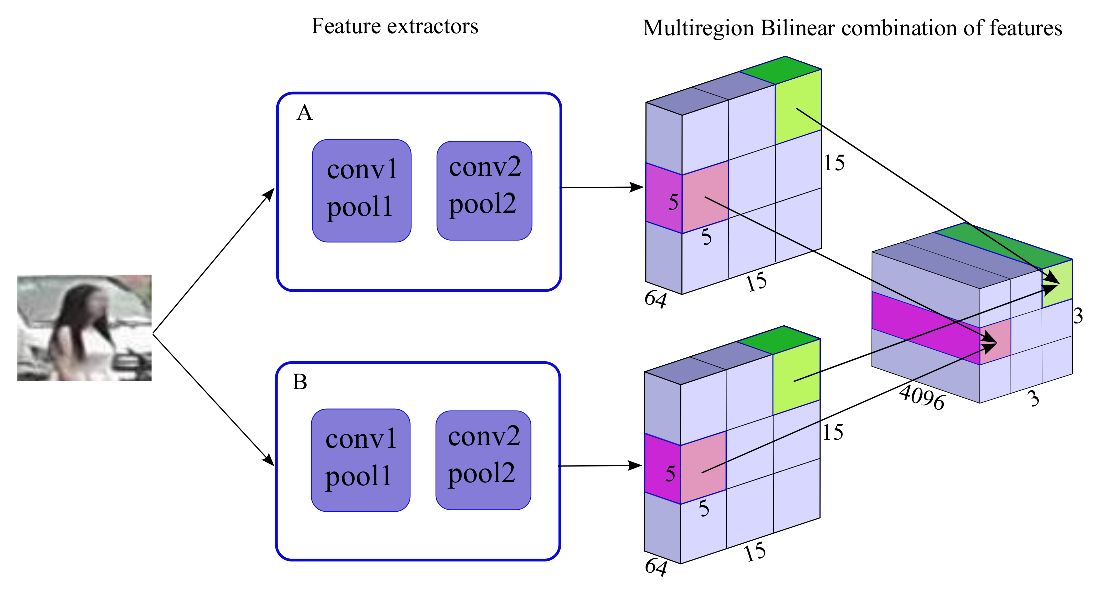
\includegraphics[width=0.7\textwidth]{\bilinearroot/figures/architecture/multiregion_bilinear.eps}\\
    (a)\\
            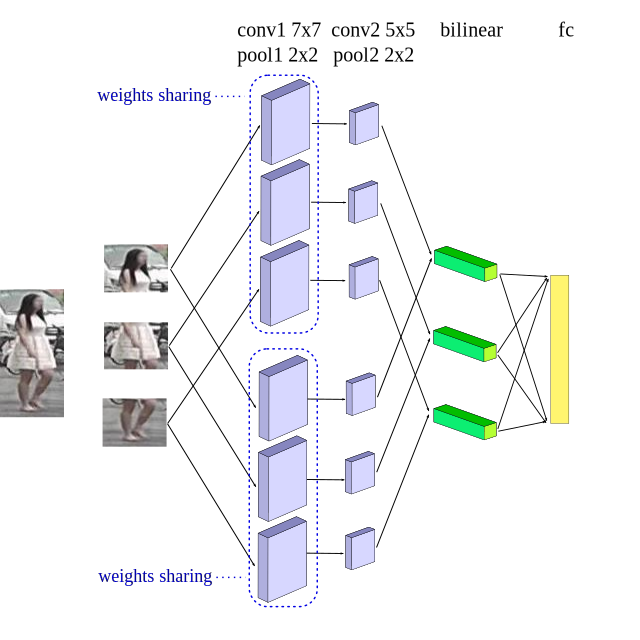
\includegraphics[width=0.7\textwidth]{\bilinearroot/figures/architecture/architecture.pdf}
            \\
    (b)\\
   
 \end{tabular}
        \caption{The proposed architecture for person re-identification: (a) - multi-region bilinear sub-network used for each of the three parts of the input image, (b) - the whole multi-region Bilinear CNN architecture that uses bilinear pooling over regions rather than the entire image. The new architecture achieves state-of-the-art performance over a range of benchmark datasets.}
        \label{fig:architecture}
    \end{center}
\end{figure*}

%\subsection{Related work}
\label{sec:related}

\subsection{Face super-resolution approaches}

Initially, super-resolution problem has been formulated for low-resolution image sequence that can be used to produced one image of higher resolution. Under this approach, reconstruction constraints are used to make sure that resulting high-resolution image is consistent with the input sequence. 
Maximum a posteriori (MAP) framework has been used in \cite{HardieBA97, SchultzS96, baker2002limits} to take into account such reconstruction constraints along with priors on the high-resolution image.

Precise image registration has been shown to be very important for multi-image \cite{HardieBA97, IraniP91, SchultzS96} and super-resolution methods but is rarely achievable for real  low-resolution data, especially for images depicting non-rigid objects such as faces. In the case of multi-image super-resolution, approximate low-parametric registration could be used instead. For single-image super-resolution, such registration with canonical pose can also be used in order to use stronger face-specific priors \cite{LiuSF07}.


Having assumed ideal image registration, Baker \emph{et al.} \cite{baker2002limits} demonstrate the effect of introducing additional recognition-based prior. The authors include it into the task formulation as additional constraints based on particular examples from  training set chosen by similarity to the regions of the input image.  Later, more advanced techniques for modeling such face-specific constraints were introduced in \cite{LiuSF07} for single-image face super-resolution. The authors decomposed such constraints to \emph{global} and \emph{local} constraints. A similar idea was also adopted in \cite{TuzelTH16} to build a ConvNet architecture for single-image face super-resolution.


%TODO : maybe elaborate on this.
%correspondence between low res and high-res patches 
%dictionary learning: faces \cite{YangWLCH12, TianT16}, direct patch correspondence :  \cite{MaZQ10}, methods are also very dependent on alignment, general and CNN :  \cite{DongLHT16} 

\subsection{Deep learning for face super-resolution}

Several recent deep learning approached \cite{TuzelTH16,ZhuLLT16,xu2017learning,huang2017wavelet} focus on single-image face super-resolution problem.
Tuzel \emph{et al.} \cite{TuzelTH16} suggested the end-to-end learning scheme to obtain high quality results even in the case of 8x down-sampling. The architecture includes two parts corresponding to global and local modeling of the face features. In the \emph{global} network, the fully-connected layers are used to capture the global face structure, while the \emph{local} part consists of convolution layers that are used to model local face features. Additionally, authors apply adversarial learning to achieve more realistic results. 
Below, we use the \textit{Perceptual loss} for the similar goal.

Xu \emph{et al.} \cite{xu2017learning} also use generative adversarial networks (GANs) \cite{goodfellow2014generative} for single-image face super-resolution. The authors introduce additional recognition-based losses. First, feature matching loss ensures that reconstructed high-resolution image and ground truth image have similar features extracted from the discriminator network. This approach resembles \textit{Perceptual losses}.  Second, multi-class discriminator was used to learn one generator network for two different domains of texts and faces. %The authors demonstrate visual improvement of combination of feature-level and GAN losses over using only GAN loss. Together these losses help to build a strong prior on generated images and achieve better qualitative and quantitative results. 


Zhu \emph{et al.}~\cite{ZhuLLT16}  proposed a cascaded scheme that includes iterative high-resolution image refinement and pose estimation from these refined images. This approach is motivated by the fact that face super-resolution and face pose estimation tasks are related, and it is easier to increase image resolution knowing the pose of the face and vice versa. Special gated architecture is introduced to effectively combine high-frequency and low-frequency information and make use of face pose estimated at previous scale levels.

Huang \emph{et al.} \cite{huang2017wavelet} use another recognition-based loss: the proposed neural network is trained to predict wavelet transform coefficients which helps to capture and match information at different scales.

All the aforementioned methods only consider single-frame face super-resolution/restoration. To the best of our knowledge, none of the recent works on deep face super-resolution consider multi-frame scenario. It should also be mentioned that methods \cite{TuzelTH16,xu2017learning,huang2017wavelet} use pre-aligned images for training and testing. (However, \cite{huang2017wavelet} demonstrate very impressive results for difficult face poses.) In contrast, we stick to 'more real' scenario when no alignment is applied to high-resolution ground-truth images before down-sample them. 


\subsection{Restoration and recognition}
%\cite{Hennings-YeomansBK08, ZhangYZNH11}
%The idea of combining the two tasks of face image restoration and face recognition has been investigated in several works


Initially, recognition was incorporated into face super-resolution in the form of face-specific priors \cite{baker2002limits, LiuSF07}. Several works considered an explicit combination of face recognition and face restoration tasks: \cite{Hennings-YeomansBK08, ZhangYZNH11}.
The proposed approaches perform recognition using a limited number of gallery images. In parallel, they reconstruct the input image and classify it based on labels of the most relevant examples found in the train set. Here we work in a different setting using a feed-forward deep neural network to produce the restored high-resolution image without using the gallery set at test time.

\subsection{Deep learning for video-based super-resolution}
As mentioned earlier, video data bring more useful information compared to isolated frames and can be used to enhance the restoration algorithms. Naturally, most recent deep learning approaches, which focus on video super-resolution \cite{LiaoTLMJ15, SongDQ16, TaoGLWJ17}, use motion estimation to align a number of subsequent frames to make use of sub-pixel motion and reveal more object details. Liao~\emph{et al.}~\cite{LiaoTLMJ15} use different optical flow methods to generate super-resolution "drafts". Such drafts can then be further combined into the final reconstruction using a number of convolutional layers. Kappeler~\emph{et al.}~\cite{KappelerYDK16} also experiment with different variants of video-based super-resolution architecture incorporating neighbouring frames alignment. 

%here it is interesting to check if Warping Subnet even changes during training => it would be possible to say that we benefit from end-to-end learring in this case.
Our idea is to adopt similar approach based on video-data and frame alignment for human faces. Importantly, we aim not only at enhancing image quality but also at preserving face identities and therefore improving face verification quality for the restored images.
 
   





%\begin{figure*}
%\begin{center}

%\includegraphics[width=\textwidth]{images/method/vgg_loss.pdf}

%\caption{General scheme of learning super-resolution with perceptual loss. Along with L2 loss, the \textit{Perceptual loss} \cite{JohnsonAF16} is used, that is the loss computed for high-level features extracted from pre-trained CNN. The weights of the pre-trained CNN are fixed during training. See \ref{sec:vgg_loss} for the details.}

%\label{fig:vgg_loss}

%\end{center}

%\end{figure*}



\section{Evaluated approaches}
\label{sect:method}
\bigskip
\indent\textbf{Face recognition for the low-quality image domain}\\
%\subsubsection{Face recognition for the low-quality image domain}
\label{sect:strategies}
In this work we consider and compare two main approaches to face recognition for surveillance data: 1) restoration-based approach and 2) domain adaptation of existing face recognition neural networks. 

We consider two facial image domains: \begin{itemize}
\item domain $T: \{X^{T}_{i} \}_{i=0}^{N_T}$ that includes low-quality facial images $X^{T}_{i}$ captured using surveillance cameras. Usually, there are no identity labels provided, as assigning identity labels is quite challenging and may not even be feasible.
\item domain $S: \{(X^{S}_{i}, Y^{S}_{i})\}_{i=0}^{N_S}$ that includes facial images $X^{S}_{i}$ harvested from the Internet. These images are usually of higher quality and are taken in good lighting conditions. We assume that the data in this domain are supplied with identity labels $Y_i$.
\end{itemize}  

According to the available labeling, we can consider two different pipelines for building face recognition systems for surveillance data. The first option is the restoration-based approach when we use transform $F^{T \rightarrow S}: T \longrightarrow S$ as a face restoration method and then apply existing recognition neural network $R^{S}$ that is pre-trained on images from the domain $S$. The second option is to use the transform $F^{S \rightarrow T}: S \longrightarrow T$ to transfer the large collections of labeled training data to the target domain of surveillance images. In this scenario, we retrain the existing face recognition networks resulting in the new adapted model $R^{T}$.

More formally, we consider the following two pipelines for face recognition in the domain $T$.  We denote $d^{T}$ and $d^{S}$ the descriptors produced by the domain-specific face recognition models $R^{T}$ and $R^{S}$. These descriptors may be used e.g.\ to identify matching and non-matching faces based on the distances between them. 
 
$F^{T \rightarrow S}: T \longrightarrow S$ and $F^{S \rightarrow T}: B \longrightarrow A$ are the image-level domain transfer mappings. In the restoration-based approach, we train the recognition model $R^{S}$ using labeled data  $\{(X^{S}_{i}, Y^{S}_{i})\}$ where $X^{S}_{i} \subseteq B$. We then test the learned model by computing the descriptors $d^{S}$ after applying the network $F^{T \rightarrow S}$:  $d^{S} = R^{S}(X^{T\rightarrow S}) = R^{S}(F^{T \rightarrow S}(X^{T}))$

In the domain adaptation approach, we train the recognition network $R^{T}$ using labeled data $\{(X^{S \rightarrow T}_{i}, Y^{S}_{i})\}$, where the training examples $X^{S \rightarrow T }_{i} = F^{S \rightarrow T}(X^{S}_i)$, $X^{S}_i \subseteq S$ are obtained by transforming the high-quality images to the low-quality domain using the learned transformation $F^{S \rightarrow T}$. In this case, we apply the learned network directly to the low-quality images by computing and working with their descriptors $d^{T} = R^{T}(X^{T})$. The two approaches are compared below.


%image describing train and test time for both schemes
\bigskip
\indent\textbf{Learning domain transfer mappings}\\
%\subsubsection{Learning domain transfer mappings}
\label{sect:domain_transfer}
We use the CycleGAN approach~\citep{ZhuPIE17} to simultaneously learn the domain transfer mappings in both directions: $ F^{T \rightarrow S}: T  \longrightarrow S$ (restoration-based approach) and  $F^{S \rightarrow T}: S \longrightarrow T$ (domain adaptation approach). Here we describe the objective functions used for learning the domain transfer architecture.

We use the variant of CycleGAN similar to the one introduced in \citep{LiuNIPS2017} as we found it resulting in more stable and visually more plausible results for our task than the original framework \citep{ZhuPIE17}. Following \citep{LiuNIPS2017}, we decompose the domain transfer mappings into the compositions of encoders and generators: $F^{T \rightarrow S} = G^{S} \odot E^{T} $ and $F^{S \rightarrow T} = G^{T} \odot E^{S} $. Here, the encoders $E^{T}$ and $E^{S}$ transfer input images to the latent space, and generators $G^{S}$ and $G^{T}$ map the input latent codes to the domains $S$ and $T$.
 
For inputs $X^{T} \subseteq T $ and $X^{S} \subseteq S $ the results of their transfer to the opposite domain will be:
\begin{equation}
    X^{T \rightarrow S} = F^{T \rightarrow S}(X^{T}; \theta^{T}_F) = G^{S}(E^{T}(X^{T}))  
\end{equation}
\begin{equation}
    X^{S \rightarrow T} = F^{S \rightarrow T}(X^{S}; \theta^{S}_F) = G^{T}(E^{S}(X^{S}))
\end{equation}

The objective function used by the CycleGAN approach for learning is composed of the two symmetric parts:
\begin{equation}
\mathcal{L} = \mathcal{L}^{T} + \mathcal{L}^{S},
\end{equation} where $\mathcal{L}^{T}$ further decomposes as:
\begin{equation}\label{eq:domain_loss}
     \mathcal{L}^{T} = \mathcal{L}_{\text{GAN}}^T + \lambda_1 \mathcal{L}_{\text{cycle}}^T + \lambda_2 \mathcal{L}_{\text{rec}}^T,
\end{equation}
while $\mathcal{L}^{S}$ has same structure as $\mathcal{L}^{T}$:
\begin{equation}\label{eq:domain_loss2}
     \mathcal{L}^{S} = \mathcal{L}_{\text{GAN}}^S + \lambda_1 \mathcal{L}_{\text{cycle}}^S + \lambda_2 \mathcal{L}_{\text{rec}}^S,
\end{equation}


We now describe each of the terms in \eq{domain_loss}.
The GAN loss serves as the optimization objective for the domain transfer: 

\begin{dmath}
\mathcal{L}_{\text{GAN}}^A = 
    \min_{\theta^{S}_F} \max_{\theta^{T}_D} \mathbb{E}_{x \sim p_{X^{T}}} \log D^{T}(x) +
    \mathbb{E}_{x \sim p_{X^{S}}} \log \big(1 - D^{T}(F^{S \rightarrow T}(x)) \big)\,
\end{dmath}


Here, $D^{T}(X;\theta^{T}_D)$ and $D^{S}(X;\theta^{S}_D)$ are discriminators for the domains $T$ and $S$ that are trained in parallel with the training of the domain transforms.

The other two terms are the so-called cycle consistency loss: 
\begin{equation}
\mathcal{L}_{\text{cycle}}^T = L_1(F^{S \rightarrow T}(F^{T \rightarrow S}(X^{T})), X^{T})  
\end{equation}
and the reconstruction loss:
\begin{equation}
\mathcal{L}_{\text{rec}}^T = L_1(G^{T}(E^{T}(X^{T})), X^{T}) 
\end{equation}
In both terms, $L_1(\cdot,\cdot)$ denotes the $L_1$ distance.

We show the results of transferring the Internet and surveillance images to the other domain in figure \ref{fig:lr_hr_gan_res_ytube_initial_degraded}. While these results look interesting, we do not analyze their visual quality, as we are ultimately interested in the recognition performance rather than obtained visually-convincing images.

\bigskip
\indent\textbf{Learning face recognition models}\\
%\subsubsection{Learning face recognition models}
\label{sect:face_recognition}
In both scenarios that we compare in this paper, we need to train a face recognition model that turns images into vectorial descriptors. This happens either in domain $S$ (in the face restoration approach) or in domain $T$ (in the domain adaptation approach).

In either case, the goal of the training is to build a deep convolutional network that converts face images to the descriptors, such that matching face images have close descriptors and non-matching face descriptors have dissimilar descriptors. We use the Binomial Deviance loss~\citep{Yi14} to perform such training \eq{bindev}. We note that the choice of a particular metric learning loss is orthogonal to our study.

Alternatively to the models trained using the setting discussed above, we also consider reusing the VGG face model trained by the authors of~\citep{parkhi2015deep} on the VGG-face dataset.
\section{Experiments}
\label{sect:experiments}

We now perform evaluation and the comparison of the two approaches and their variants. 


\bigskip\indent\textbf{Datasets and protocols} 
%\subsubsection{Datasets and protocols}

\label{sect:datasets}

\bigskip\indent\textbf{Surveillance data}\\
%\subsubsubsection{Surveillance data}
\label{sect:surveillance}
For the surveillance image domain ($T$, as denoted in \sect{strategies}), we have obtained a surveillance dataset comprising faces from five cameras in Moscow subway. Our dataset consists of two subsets of images, denoted as \texttt{LR} (low-resolution) and \texttt{HR} (high-resolution) according to their size in pixels. Sizes are calculated as the face bounding box heights. Mean face heights for \texttt{LR} and \texttt{HR} subsets were $49.72$ and $106.19$ pixels correspondingly. The \texttt{LR} images range from $37$ to $63$ pixels, and \texttt{HR} images from $75$ to $224$. The DLib \cite{dlib09} library was used for face detection and subsequent alignment. 
 
Generally, the identities of people occurring in the video are unknown, and therefore we mine matching faces in the dataset by considering temporal tracks in videos. We assume that face images from different tracks are non-matching. The matching pairs then correspond to pairs of faces from the same track, such that one image belongs to the LR subset and the other belongs to the HR subset. Columns 1 and 3 in \fig{lr_hr_gan_res_ytube_initial_degraded} show some examples of matched pairs. Usually, the quality of face images increases when the person approaches the camera, and therefore \texttt{HR}-subset images are often (but not always) visually better than those present in the \texttt{LR} subset. The division into \texttt{LR} and \texttt{HR} subsets is introduced to ensure that the matched pairs of frames correspond to distinct frames of the temporal tracks. We stress that the mined matching pairs are used for evaluation (testing) only and are not used for training of any networks in our experiments.

We use $100$ identities that are present in both \texttt{LR} and \texttt{HR} for parameter validation and $100$ identities for test. For each of the test identity, there is a pair of matching tracks (one LR track and one HR track). The goal of algorithms is then to build descriptors that would be similar for frames coming from the HR and the LR tracks of the same identity, and would be dissimilar for the HR and the LR tracks corresponding to different identities.

$7,535$ images of identities not present in the test set are used for training the unsupervised domain transfer described in \sect{domain_transfer} (tracking-based information was not used to train the ConvNets). The mean number of frames for each identity in \texttt{LR} and \texttt{HR} test data are $18.62$ and $17.72$ correspondingly.
 
 To evaluate the recognition quality, we match identities across the \texttt{LR} and \texttt{HR} in the following way: we calculate the cosine similarity between the frame set $t_{id_1}^{LR}$ of identity $id_1$ and the frame set, $t_{id_2}^{HR}$ of identity $id_2$ by averaging the similarities of each pair of frames: 

 \begin{align}
     S(t_{id_1}^{LR},t_{id_2}^{HR}) = \sum_{i=0, j= 0}^{|t_{id_1}^{LR}|, |t_{id_2}^{HR}|} S(f_{id_1,i}^{LR},f_{id_2,j}^{LR} ), \\
     S(f_{id_1,i}^{LR},f_{id_2,j}^{LR} ) =  cos(d_{id_1,i}^{LR},d_{id_2,j}^{LR}),
 \end{align}
 where $d_{id_1,i}^{LR}$,$d_{id_2,j}^{HR}$ are the descriptors of the corresponding frames calculated by face recognition neural network $R$ \ref{sect:face_recognition}.
%f_{id_1,i}^{low} \subseteq t_{id_1}^{low} , %f_{id_2,j}^{low} \subseteq t_{id_1}^{low}

%\subsubsection{Evaluation metrics}
\bigskip\indent\textbf{Evaluation metrics}\\
We focus our evaluation on the surveillance data domain. As already mentioned above, during evaluation, we compare pairs of \textit{tracks}, where the first track comes from the \texttt{LR} subset and the second track comes from the \texttt{HR} subset. 

When comparing the two tracks using the recognition metrics, we match all possible pairs of frames and compute the mean average cosine similarity between the computed descriptors over all pairs (more sophisticated schemes involving minimal pairs did not result in better performance). Depending on whether the mean average cosine similarity is higher or lower than a certain threshold $\tau$, we treat a certain pair of tracks as matching or non-matching.

 By considering various $\tau$, we then compute the \textit{ROC curve}, the area under the ROC curve (ROC AUC), the $100$\% - EER (Equal Error Rate) statistics, and the average precision (AP) metrics. 


\bigskip\indent\textbf{Internet data}\\
%\subsubsubsection{Internet data}
For the Internet image domain ($S$, as denoted in \sect{strategies}) we use two face recognition datasets: YouTube Faces (YTF) \cite{WolfHM11} and the VGG Face datasets \cite{parkhi2015deep}. %Celeb-A \cite{liu2015faceattributes},

%todo check
%The Celeb-A dataset~\cite{liu2015faceattributes} consists of $202,599$ images of high quality and is used for training CycleGAN-based  domain transfer described in \sect{domain_transfer}. 


% ----------------to main intro
 The Youtube Faces (YTF) dataset~\cite{WolfHM11} and the VGG Face dataset~\citep{parkhi2015deep} are used for the finetuning of the face recognition neural network as described in \sect{face_recognition}.

%YTF consists of $3,425$ videos of $1,595$
% people collected from YouTube, with an average of 2 videos per identity. The VGG Face dataset contains $2,6$M images of $2,622$ identities. 

We show that face recognition improves, when using our CycleGAN-based data augmentation when trained on either YTF or VGG Face. Generally, YTF and VGG Face represent two different types of face images that can be mined from the Internet (with YTF having lower quality).





%All the images in the four mentioned datasets are aligned in the same way: DLib is used for feature detection and alignment by $3$ eyes and nose feature-points, so that their target positions are the following :


\bigskip\indent\textbf{Compared variants of recognition networks} \\
%\subsubsection{Compared variants of recognition networks}
\label{sect:ft}
We compare the following adaptation/transfer strategies for training the recognition networks:
\begin{itemize}

\item \textit{no ft} -- the pre-trained VGG-face model~\cite{parkhi2015deep} with no re-training is used to compute descriptors of the surveillance-domain images.


\item \textit{ft initial} -- the VGG-face model is fine-tuned using the original version of the YTF or the VGG Face datasets (no domain adaptation). 

\item \textit{ft degraded} -- the VGG-face model fine-tuned using the degraded version of the YTF or VGG Face datasets transferred to the target (surveillance) domain (using domain adaptation),

\item \textit{ft union} -- the VGG-face model fine-tuned using \textbf{both} the initial and the degraded versions  of the YTF or VGG Face datasets (using domain adaptation). 

\end{itemize}

The YTF dataset images and the corresponding degraded images are shown  in \fig{lr_hr_gan_res_ytube_initial_degraded} (the two last columns).
%The two last variants \textit{ft degraded} and \textit{ft union} perform domain adaptation, as all or part of the training data are transferred to the target domain.



\bigskip\indent\textbf{Training details}  \\
%\subsubsection{Training details}
\label{sect:training}
The CycleGAN-based domain transfer consists of $3$ types of modules (see \sect{domain_transfer}).
Encoders $E_T$ and $E_S$ have the following architecture:
\begin{center}
\begin{scriptsize}
\begin{tabular}{l | c c c c c c c}
\hline
  \#conv layer      &1   &2      &3    &4     &5    &6    &7     \\
  num of filters    &32  &64     &128  &128   &128  &128  & 128  \\
  kernel size       &3   &3      &3    &3     & 3   &3    &3     \\
  stride/pad        &1/0 &2/1    &2/1  &1/1   &1/1  &1/1  & 1/1  \\
  \#res block       & -  & -     & -   & 0    &0    &1    &1     \\
\hline
\end{tabular}
\end{scriptsize}
\end{center}
\vspace{0.5em}

% EncShared(
%   (from_img): ModuleList(
%     (0): Conv2d(3, 32, kernel_size=(1, 1), stride=(1, 1))
%   )
%   (enc_blocks): ModuleList(
%     (0): Sequential(
%       (0): Conv2d(32, 64, kernel_size=(3, 3), stride=(2, 2), padding=(1, 1), bias=False)
%       (1): InstanceNorm2d(64, eps=1e-05, momentum=0.99, affine=True)
%       (2): LeakyReLU(0.01, inplace)
%     )
%     (1): Sequential(
%       (0): Conv2d(64, 128, kernel_size=(3, 3), stride=(2, 2), padding=(1, 1), bias=False)
%       (1): InstanceNorm2d(128, eps=1e-05, momentum=0.99, affine=True)
%       (2): LeakyReLU(0.01, inplace)
%     )
%   )
% )

% Enc(
%   (enc_blocks): ModuleList(
%   )
%   (res_blocks): ModuleList(
%     (0): ResBlock(
%       (model): Sequential(
%         (0): Conv2d(128, 128, kernel_size=(3, 3), stride=(1, 1), padding=(1, 1), bias=False)
%         (1): InstanceNorm2d(128, eps=1e-05, momentum=0.99, affine=True)
%         (2): LeakyReLU(0.01, inplace)
%         (3): Conv2d(128, 128, kernel_size=(3, 3), stride=(1, 1), padding=(1, 1), bias=False)
%         (4): InstanceNorm2d(128, eps=1e-05, momentum=0.99, affine=True)
%       )
%     )
%     (1): ResBlock(
%       (model): Sequential(
%         (0): Conv2d(128, 128, kernel_size=(3, 3), stride=(1, 1), padding=(1, 1), bias=False)
%         (1): InstanceNorm2d(128, eps=1e-05, momentum=0.99, affine=True)
%         (2): LeakyReLU(0.01, inplace)
%         (3): Conv2d(128, 128, kernel_size=(3, 3), stride=(1, 1), padding=(1, 1), bias=False)
%         (4): InstanceNorm2d(128, eps=1e-05, momentum=0.99, affine=True)
%       )
%     )
%   )
% )

The architecture of generators $G_T$, $G_S$ is as follows:
\begin{center}
\begin{scriptsize}
\begin{tabular}{l | c c c c c c c}
\hline
  \#conv layer      &1      &2    &3     &4    &5    &6    & 7 \\
  num of filters    &128    &128  &128   &128  &64   &32   & 3 \\
  kernel size       &3      &3    &3     & 3   &3    &3    & 1 \\
  stride/pad        &1/1    &1/1  &1/1   &1/1  &1/1  &1/1  & 1/0  \\
  \#res block       &0      &0    &1     &1    &-    &-    & -  \\
\hline
\end{tabular}
\end{scriptsize}
\end{center}
\vspace{0.5em}

Instance normalization~\cite{UlyanovVL17} and Leaky ReLU~\cite{HeZRS15} with negative slope set to $0.01$ are inserted after each of the convolution layers. Except for the last layers of $G_T$ and $G_S$, where \texttt{tanh} non-linearity is used (for the subsequent feeding of the result into the discriminator). To keep the input image size unchanged,  $\times 2$ nearest neighbor upsampling is done before the convolutions $3$ and $4$.
All input images are normalized to $64\times64$ pixels (output images are therefore of the same size). 


% Dec(
%   (to_img): ModuleList(
%     (0): Sequential(
%       (0): Conv2d(32, 3, kernel_size=(1, 1), stride=(1, 1))
%       (1): Tanh()
%     )
%   )
%   (upsample): Upsample(scale_factor=2, mode=nearest)
%   (res_blocks): ModuleList(
%     (0): ResBlock(
%       (model): Sequential(
%         (0): Conv2d(128, 128, kernel_size=(3, 3), stride=(1, 1), padding=(1, 1), bias=False)
%         (1): InstanceNorm2d(128, eps=1e-05, momentum=0.99, affine=True)
%         (2): LeakyReLU(0.01, inplace)
%         (3): Conv2d(128, 128, kernel_size=(3, 3), stride=(1, 1), padding=(1, 1), bias=False)
%         (4): InstanceNorm2d(128, eps=1e-05, momentum=0.99, affine=True)
%       )
%     )
%     (1): ResBlock(
%       (model): Sequential(
%         (0): Conv2d(128, 128, kernel_size=(3, 3), stride=(1, 1), padding=(1, 1), bias=False)
%         (1): InstanceNorm2d(128, eps=1e-05, momentum=0.99, affine=True)
%         (2): LeakyReLU(0.01, inplace)
%         (3): Conv2d(128, 128, kernel_size=(3, 3), stride=(1, 1), padding=(1, 1), bias=False)
%         (4): InstanceNorm2d(128, eps=1e-05, momentum=0.99, affine=True)
%       )
%     )
%   )
%   (dec_blocks): ModuleList(
%     (0): Sequential(
%       (0): Conv2d(128, 64, kernel_size=(3, 3), stride=(1, 1), padding=(1, 1))
%       (1): LeakyReLU(0.01, inplace)
%     )
%     (1): Sequential(
%       (0): Conv2d(64, 32, kernel_size=(3, 3), stride=(1, 1), padding=(1, 1))
%       (1): LeakyReLU(0.01, inplace)
%     )
%   )
% )


%Finally, discriminators $D_A$ and $D_B$ were derived from the
%VGG-face model~\cite{parkhi2015deep}, which was used for calculating face descriptors, leading to the following archiecture:
Finally, discriminators $D_A$ and $D_B$ have the following architecture: 
\begin{center}
\begin{scriptsize}
\begin{tabular}{l |c c c c c }
\hline
  \#conv layer      &1      &2    &3     &4    &5  \\
  num of filters    &64     &128  &256   &256  &1  \\
  kernel size       &3      &3    &3     & 3   &3  \\
  stride/pad        &2/1    &2/1  &2/1   &2/1  &1/0\\
\hline
\end{tabular}
\end{scriptsize}
\end{center}
\vspace{0.5em}
Leaky ReLU \cite{HeZRS15} with negative slope parameter set to $0.01$ is used as an activation. The final fully-connected layer with one output unit is added to $D_A$ and $D_B$.


% Dis(
%   (to_pred): ModuleList(
%     (0): Conv2d(256, 1, kernel_size=(1, 1), stride=(1, 1))
%     (1): Conv2d(256, 1, kernel_size=(1, 1), stride=(1, 1))
%   )
%   (blocks): ModuleList(
%     (0): Sequential(
%       (0): Conv2d(128, 256, kernel_size=(3, 3), stride=(2, 2), padding=(1, 1))
%       (1): LeakyReLU(0.01, inplace)
%     )
%     (1): Sequential(
%       (0): Conv2d(256, 256, kernel_size=(3, 3), stride=(2, 2), padding=(1, 1))
%       (1): LeakyReLU(0.01, inplace)
%     )
%   )
% )


According to the strategies described in \sect{ft}, we fine-tune the VGG-face model, having added new $128$-dimensional embedding layer instead of the initial classification layer (\textit{fc8}). All the results are reported for the \textit{fc7} layer though, as we found it to work better across all compared methods.

ADAM optimization~\cite{Kingma14} was used for both optimization objectives of the domain transfer task and the face recognition task, the learning rates were set to $1e-4$ and $1e-7$ correspondingly. Batch sizes were $16$ and $64$. Learning processes took $50$ epochs for the domain transfer,  and from $80$ to $200$ epochs for the face recognition task. Parameters $\lambda_1$ and $\lambda_2$ were set to $10$ in the loss \eq{domain_loss}. Parameters $\alpha$, $\beta$ and $C$ of the loss \eq{bindev} were set to $2$, $0.5$ and $10$.

For training the face recognition models described in \sect{ft}, the training batches had the following structure: in each batch, there were up to $3$ examples for each class for the VGG Face dataset and up to $10$ examples for the YTF dataset. For the \textit{ft union} model, each training batch was formed out of the examples of one of the domains. The sampling process alternated between the domains at each iteration.


  
 \begin{figure}
  \centering
    \includegraphics[width=\linewidth]{Chapters/face/Fig3.eps}
    \caption{The ROC curves for our face recognition models for different types of test data. Left -- \textit{no ft} model, test data transformation (the curve is denoted by 'restored') improves recognition. Middle -- \textit{ft initial}, the results for test data transformation are not clearly better than the results for initial images. Right -- \textit{ft union} model, the best results are for initial test data, without transformation. See \ref{sect:restoration_comparison} for the details. }\label{fig:roc_oxford_gan_vs_initial}
  \end{figure}

\bigskip\indent\textbf{Does restoration help recognition?} \\
%\subsubsection{Does restoration help recognition?}
\label{sect:restoration_comparison}
We start by assessing the improvement that the restoration process brings to the recognition. For this we evaluate the performance of the three different recognition networks discussed above, when they are applied either to untransformed surveillance-domain images or to surveillance-domain images transformed to the Internet image domain (using the learned mapping $F^{T \rightarrow S}$). See  \fig{lr_hr_gan_res_ytube_initial_degraded} for the example results of the Internet domain  transfer.

The ROC-curves in  \fig{roc_oxford_gan_vs_initial} shows that while the restoration process helps for the \textit{no ft} network, it actually \textit{hurts} for the better-performing \textit{ft initial} and \textit{ft union} networks. While trying to improve the results of the reverse transfer, we have also tried to transfer only the LR subset of the training images, while keeping the HR subset intact, but this lead to uniformly worse results.

We conclude that restoration does not necessarily help the recognition process in our setting. 



\begin{figure}
 \centering
    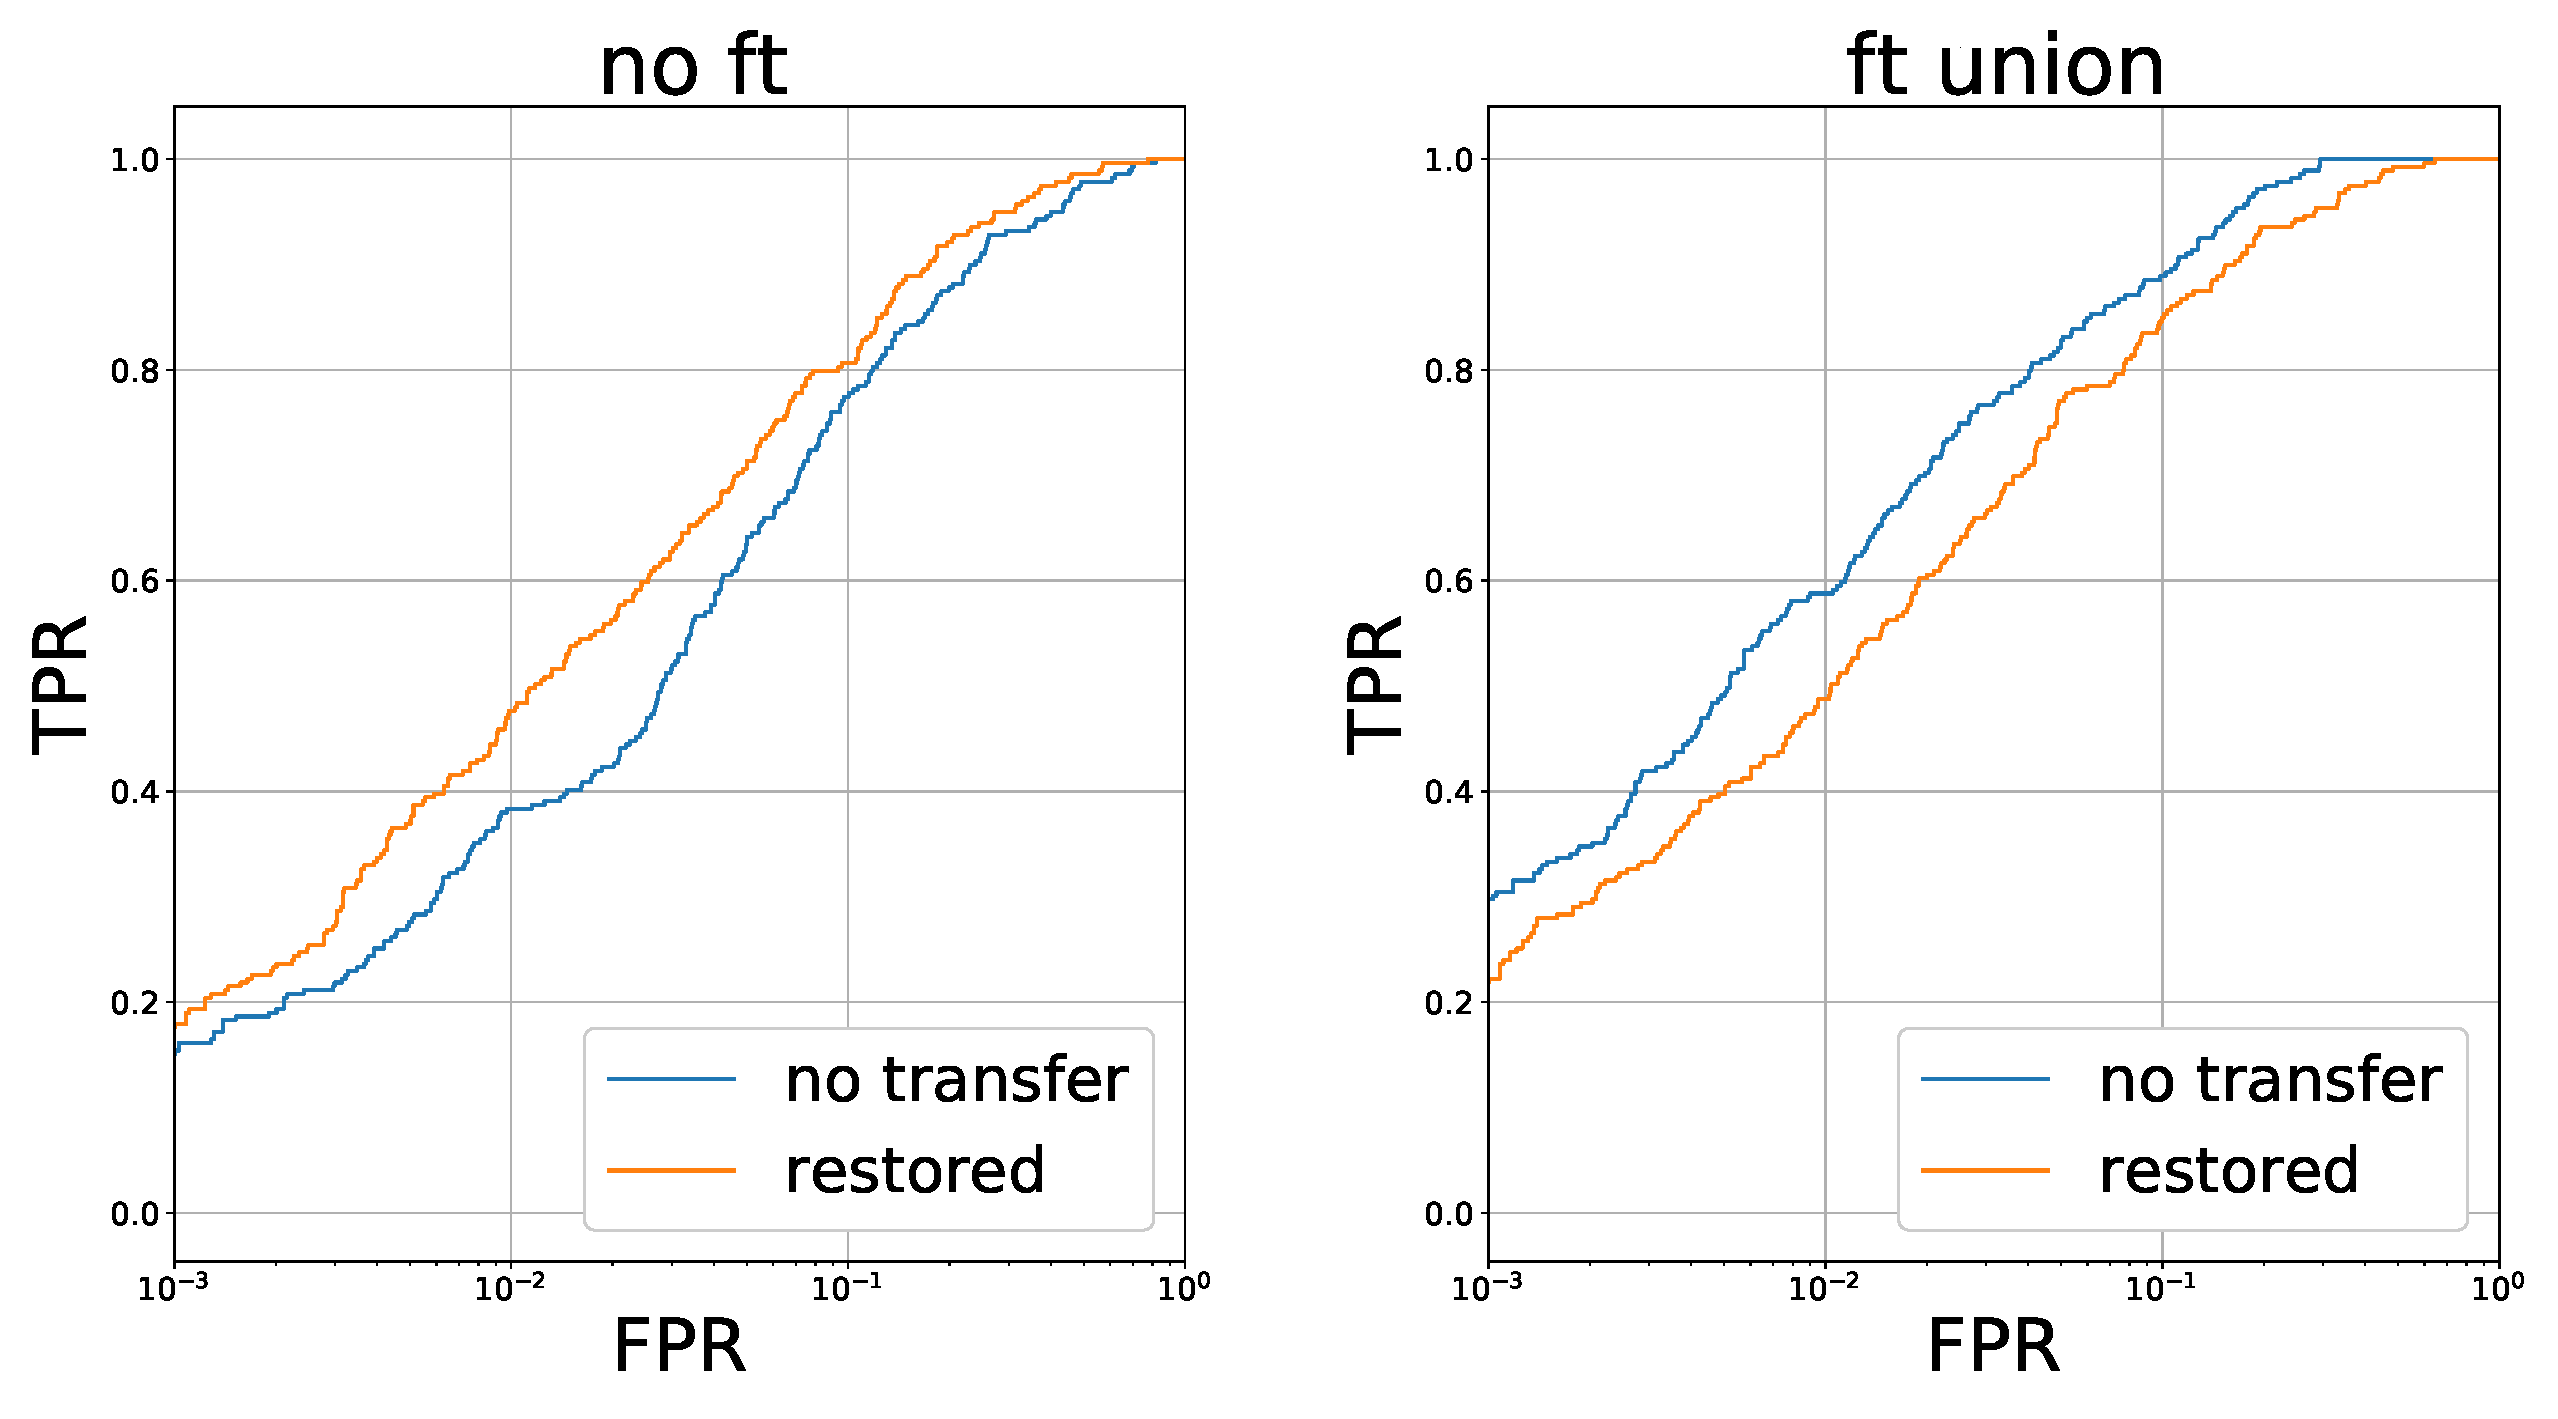
\includegraphics[width=\linewidth]{Chapters/face/Fig4.eps}
    \caption{The change of the recognition metrics for our surveillance validation set. \textit{ft degraded} and \textit{ft union} models that use our image-level domain adaptation overfit less than \textit{ft initial} that use only the initial Internet-domain data. The improvement is consistent across the two cases when VGG face and YTF datasets were used as Internet image data. See subsection \ref{sect:ft} for the models description.}\label{fig:validation_ytube}
  \end{figure}
  
  \begin{figure}

  \centering
    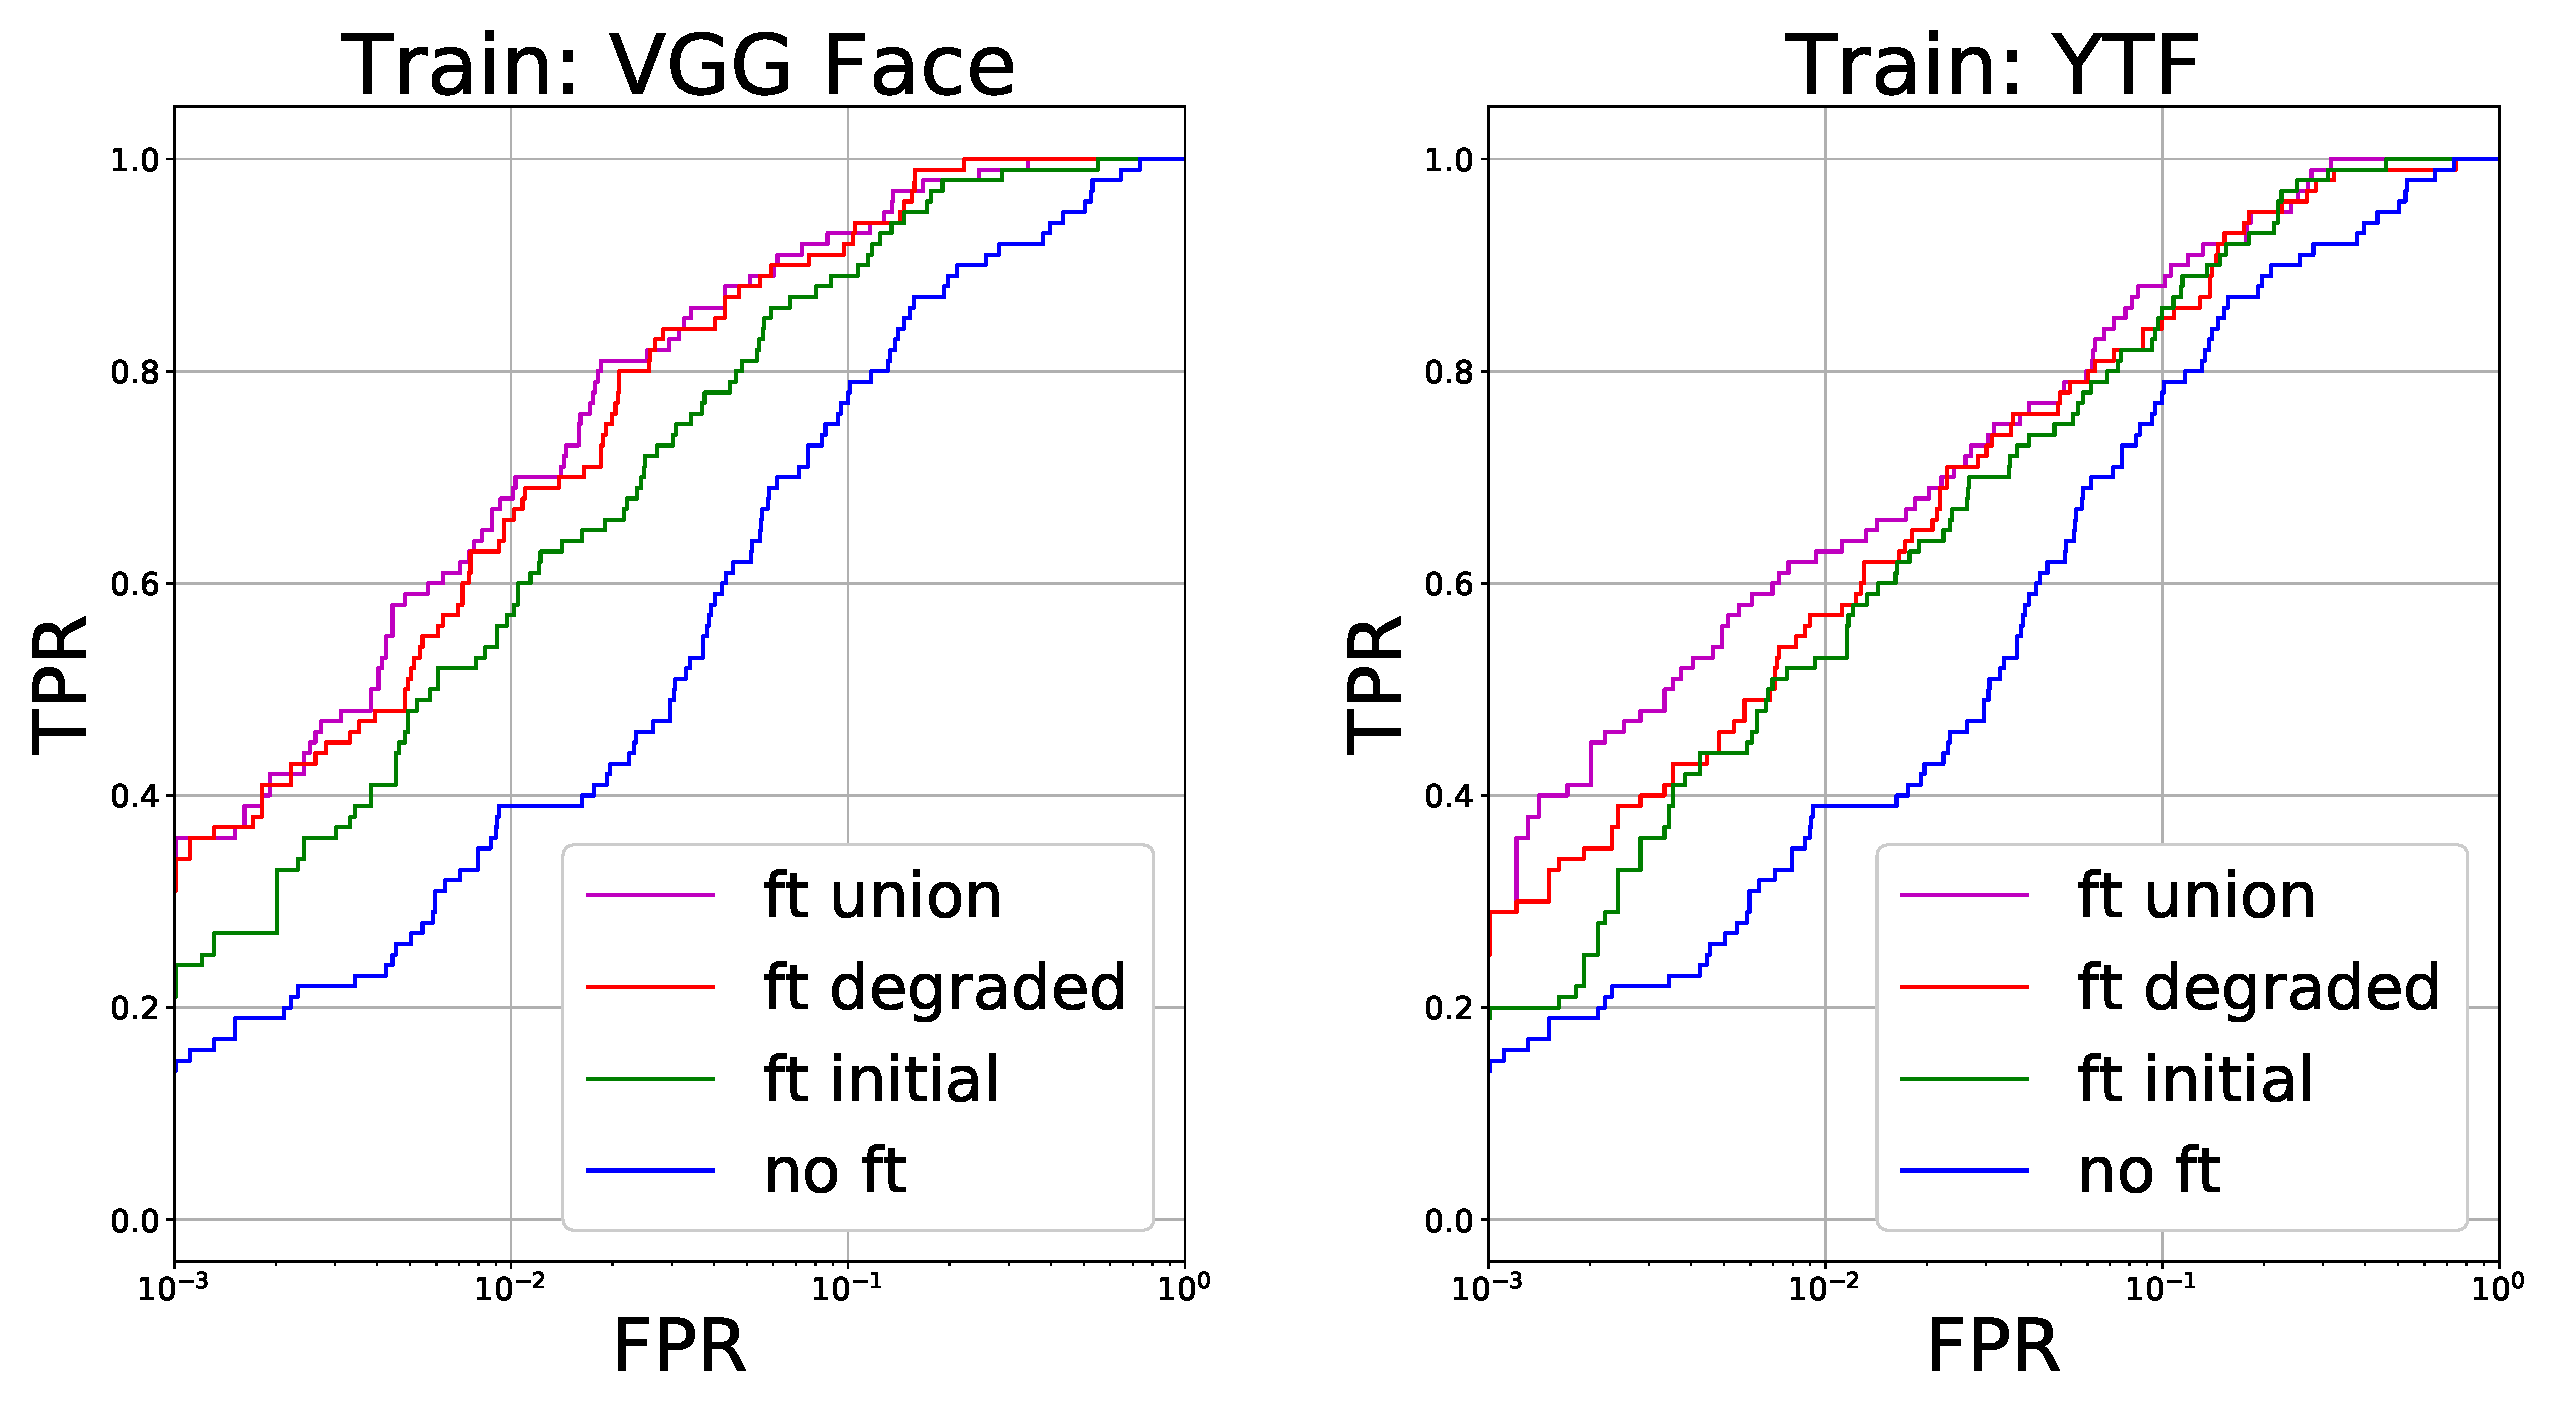
\includegraphics[width=\linewidth]{Chapters/face/Fig5.eps}
    \caption{The ROC curves for the fine-tuning strategies described in \sect{ft}. Our surveillance data is used for test. \textit{ft degraded} and \textit{ft union} models that use our image-level domain adaptation are better than other models. }\label{fig:roc_oxford_ytube}
  \end{figure}
  
 
\begin{table}
\flushbottom

\centering
\caption{Quality metrics for different face recognition models compared in this work (\ref{sect:ft}). The best model is \textit{ft union}, it is trained on both initial and degraded data.}
\label{tab:comparison}
\resizebox{\columnwidth}{!}{
\begin{tabular}{|c|c|c|c|c|c|c|}
\hline
\multicolumn{1}{|l|}{}   & \multicolumn{6}{c|}{Train datasets}                      \\ \hline
\multicolumn{1}{|l|}{}   & \multicolumn{3}{c|}{YTF} & \multicolumn{3}{c|}{VGG Face} \\ \hline
Fine-tuning type & 100\%$-$eer & roc auc & AP & 100\%$-$eer   & roc auc   & AP  \\ \hline
no ft                    &  84.73 & 91.52 & 25.98 &   84.73 & 91.52 & 25.98  \\ \hline
ft initial               &  88.52 & 95.67 & 42.38 &  89.32 & 96.62& 44.10  \\ \hline
ft degraded              &  87.03         & 95.53 &  47.02 & 90.28 &\bf{97.84} &53.33  \\ \hline
ft union                 &  \bf{89.41}    &   \bf{96.45} &\bf{50.91}&    \bf{91.31} &97.80 &\bf{54.89}   \\ \hline
\end{tabular}
}
\end{table}

  
 
%\subsubsection{Does domain adaptation help recognition?}
\bigskip\indent\textbf{Does domain adaptation help recognition?} \\
\label{sect:results}
We now consider the second scenario based on domain adaptation and thus compare the performance of different recognition networks described above on surveillance data. Our findings for image level domain adaptation are summarized in Table~\ref{tab:comparison}, which shows metric values for the compared training settings, and \fig{validation_ytube}, which shows validation metrics changes during training. Finally, \fig{roc_oxford_ytube} shows the final ROC curves.

The following can be observed. First, fine-tuning the VGG Face model on either VGG Face dataset or the YTF dataset using the BinDev loss (\textit{ft initial}) lead to a considerable improvement over the original state of the network.
Furthermore, we found that fine-tuning in the \textit{ft degraded} setting is clearly beneficial compared to \textit{ft initial} setting in the case of the VGG Face training dataset, and a little bit better for the YTF training data, overall making a case for image-level domain adaptation. The results of the \textit{ft union} setting are uniformly better than \textit{ft initial} and \textit{ft degraded} suggesting that the automatically degraded data are a useful augmentation, but that the original data should not be discarded. 
Finally, \fig{tsne} gives an additional evidence of the success of domain adaptation. It shows that the feature distribution of our surveillance data is more intermixed with those of the degraded version of the YTF dataset than its initial version. This demonstrates the relevance of the suggested augmentation (via image-level domain adaptation).



% \subsubsection{Comparison to the reverse domain transfer}
% \label{sect:restoration_comparison}

% We have also investigated the restoration-based approach (\sect{strategies}), using the reverse mapping $F^{S \rightarrow T}$ that also comes out as the result of training the model \ref{sect:domain_transfer}. 
% Here we test our previously trained face recognition models (described in  \sect{ft}) on different variants of test data. See  \fig{lr_hr_gan_res_ytube_initial_degraded} for the example results of the Internet domain  transfer.

% We have evaluated the effect of such reverse transfer to the higher-quality domain at test term for the \textit{no ft}, \textit{ft initial}, and \textit{ft union} networks described in the previous subsection. The ROC-curves in  \fig{roc_oxford_gan_vs_initial} shows that while the reverse transfer helps for the \textit{no ft} network, it actually hurts for the better working \textit{ft initial} and \textit{ft union} networks. While trying to improve the results of the reverse transfer, we have also tried to transfer only the LR subset of the training images, while keeping the HR subset intact, but this lead to uniformly worse results.

%in the case of the pre-trained VGG face network (\textit{no-ft}), transferring low-quality test images into the Internet data domain improves recognition. Nevertheless, if we use one of the fine-tuned models for recognition, the results for the initial test images are not worse than those for transferred images. Moreover, ROC curve for initial test images is the highest for our best \textit{ft union} model as shown in \ref{fig:roc_oxford_gan_vs_initial}-right.



%\subsubsection{Comparison to feature-level domain adaptation}

\bigskip\indent\textbf{Comparison to feature-level domain adaptation} \\
\label{sect:grl}
We have additionally compared our image-level domain adaptation (all the experiments and discussions above) to the feature-level domain-adversarial adaptation approach described in \chapt{gradrev}. Tuning this approach required some effort (several modifications from the settings of \chapt{gradrev} were needed to make such adaptation work). We thus built a DANN (Deep Adversarial Neural Network) based on the VGG-face network. The  domain classifier consists of three fully-connected layers: $512$ units in the first two layers (Leaky ReLU \cite{HeZRS15} non-linearities were used) and one classification layer with $1$ unit. Dropout with $0.5$ probability was inserted before the classification layer. The Gradient Reversal layer is attached after the \textit{fc6} layer of VGG-face. We found that schedule for the adaptation parameter  $\lambda$ is very important for this task. Instead of the schedule suggested in \chapt{gradrev} (which did not lead to good results in our comparison), we set $\lambda$ to $1e-3$ for the first $20$ epochs and then increased it to $1e-2$. 

Using the scheme described above when training on the VGG Face dataset, we have achieved the following results: $100$\% - EER was $88.64$, ROC AUC was $96.69$ and the average precision was $52.11$. This is better than the results of our \textit{ft initial} setting, but worse than those of \textit{ft degraded} and \textit{ft union} settings (for the last, the results are $91.31$, $97.80$ and $54.89$ correspondingly). Other setting for feature-level domain adaptation that we have tried lead to worse results.






  
  
  
  


\begin{figure}
\includegraphics[height=0.76\textheight]{\bilinearroot/figures/market_random.png}
\caption{The result of the proposed architecture on the Market-1501 dataset for a random subset of queries. The queries are shown on the left, and the remaining images in each row show the closest matches in the gallery dataset.}
\label{fig:market_retrieval}
\end{figure}

\subsection{Summary}
\label{sec:summary}
In this work we present a deep neural network for multi-frame face super-resolution that performs alignment, reconstruction and recognition in holistic manner and learns respective modules in the end-to-end fashion. We evaluate different variants of the proposed architecture including single-image baseline. In the experiments on YouTube Faces dataset, we demonstrate the advantages of having the alignment module in the system. In the presence of alignment, we observe the improvement both in visual quality (confirmed by the user study) and in the face recognition accuracy over the single frame baselines and the single frame system \cite{ZhuLLT16}. 




%\newcommand{\root}{Chapters/face}

\chapter{Getting Off the Internet: Practical Domain Adaptation for Face Recognition}
\label{chapt:wildface_}


\section{Motivation}
%face
For face recognition, one important cross-domain scenario is related to using powerful models pretrained on professional photographs for surveillance data. As it has been already mentioned in \sect{face}, large-scale training datasets for face recognition most often include high-quality images that are very different from those captured by surveillance systems. In person re-identification, the domain difference comes mainly from the illumination condition variations between the camera sets (if the difference of the camera positions is put aside). In contrast,  surveillance face recognition implies a complex domain shift caused by a combination of low resolution, compression and illumination conditions. 


In particular, in this chapter we study the unsupervised domain adaptation scenario, where face recognition is trained using an annotated Internet face dataset and an unannotated dataset of faces collected from a surveillance camera network with low image quality. We mostly focus on the recent class of methods that consider domain-adaptation at the image level. We thus investigate how image transformation achieved with recent unsupervised image transformation techniques such as CycleGAN (\cite{ZhuPIE17}) can be used for face recognition under strong domain shifts. 

We compare and evaluate several strategies, such as transferring test data to the Internet image domain,  transferring training data to the target domain followed by retraining the network. As a baseline, we also compare to adversarial domain adaptation at feature level described in \chapt{gradrev}.% \cite{GaninUAGLLML16}. 

Our comparison suggests that image transformation (without explicit modeling of separate degradation factors) can be used for unsupervised domain adaptation of face recognition. We, however, demonstrate that special care needs to be taken in order to make such domain adaptation work better than baselines, and come up with practical suggestions on how such improvement can be achieved.

%model
% Since the CycleGAN \cite{cyclegan} architecture for image-to-image translation and stylization appeared, domain adaptation has become one of its active fields of application. This approach differs from the feature-level domain adaptation techniques of \cite{LongC0J15} and \cite{tzeng2014deep} or the method presented in the \chapt{gradrev}, because rather than finding deep domain-invariant representations, it works on the pixel level and aims at building mappings between the image domains. Thus the domain adaptation is done in two steps: building a mapping the source domain to target and retraining the predictor on the transferred source data. (Although it is also possible to combine these two steps into one optimization process.)%cycada

% %pedestrians
% For person re-identification, the pixel-level domain adaptation with CycleGAN has been applied in several recent works \cite{} (after the results of the \chapt{gradrev} were published). Some of them consider different datasets as domains, others aim at utilising synthetic re-identification data to improve the results on real data \cite{}. As demonstrated by these works, image-to-image translation may help a lot to overcome the illumination differences between the source and target camera sets. %Still, to the best of our knowledge, there are no works approaching face recognition for surveillance data.

% This chapter demonstrates the performance of the pixel-level domain adaptation approach based on CycleGAN model in the presence of an extreme domain shift between the usual face recognition training data and surveillance data. The considered surveillance data are harvested from $6$ surveillance cameras in the Moscow subway. Two publicly available face recognition datasets of different image quality are considered for the source domain. The approach is compared to several important baselines, including the reverse translation of the target images back to the source domain and the feature-level domain adaptation suggested in this chapter.

%The remainder of the chapter is organized as follows. Image-level domain transfer and face recognition methods are described in \sect{method}.  We define the variants of the training data augmentation compared in this work in \sect{ft}. Then we give the implementation details in \sect{training}. The quantitative comparisons of the described methods and baselines are presented in \sect{results}. Finally, we conclude the work with discussion and summary in \sect{conclusion}.



%\titlerunning{Short form of title}        % if too long for running head



% \begin{abstract}
% Face recognition in real surveillance scenarios is challenging due to the presence of complex degradation factors. At the same time, the easiest-to-collect and the biggest available training data for face recognition come from the Internet, where images and video frames have higher quality, higher resolution, and better lighting. In this work, we study training face recognition systems under such domain shift. We show that CycleGAN technique can be utilized for transferring labeled training data into the target domain of surveillance camera, and that the transferred data can be used to train face recognition in the new domain. We compare this approach to several baselines including the domain transfer in the opposite direction to turn test data directly to the high-quality domain. Our comparison and evaluation allow us to come up with a viable strategy for training face recognition in surveillance data.
% \keywords{face recognition \and surveillance \and domain adaptation}
% % \PACS{PACS code1 \and PACS code2 \and more}
% % \subclass{MSC code1 \and MSC code2 \and more}
% \end{abstract}


%\subsection{Introduction} Face recognition systems have seen a great progress over the last several years with super-human recognition accuracy attainable in many scenarios. However, the accuracy of recognition degrades very significantly when dealing with very low resolution faces. In such conditions, the tasks of recognition and increasing the effective resolution (\textit{super-resolution}) become intertwined and necessitate joint solution. Indeed, developing  super-resolution techniques without regard for recognition often leads to face \textit{hallucination}, i.e.\ a process that creates plausibly looking faces lacking personal specifics. On the other hand, super-resolution has been known to benefit from recognition for a long time \cite{baker2002limits}.

\begin{figure}[t]
%\begin{wrapfigure}{i}{0.5\textwidth}
\includegraphics[width=\columnwidth]{\srroot/images/ytube/teaser.png}
\caption{Results of different super-resolution convolutional networks on samples from the Youtube Faces (YTF) dataset. From left to right: ground truth, bicubic upsampling,  single-frame superresolution, super-resolution from 25 frames without alignment (ours), super-resolution from 25 frames with warping subnetwork (ours).}
\label{fig:teaser}
%\vspace{10pt}
\end{figure}



While single-image super-resolution has recently drawn considerable attention \cite{ZhuLLT16, TuzelTH16}, super-resolution over large magnification factors can benefit significantly from information accumulated over multiple images, e.g.\ using adjacent frames in a surveillance stream or a video. Traditionally, multi-frame super-resolution has required rigid or non-rigid alignment with sub-pixel accuracy \cite{capel2003computer}. 
At the same time, faces have complex and deformable shapes leading to complex two-dimensional motion patterns which makes motion estimation hard to accomplish at sub-pixel precision. Generally, such precise alignment cannot be accomplished using low-level cues alone, and therefore requires high-level understanding/recognition of face geometry.



Motivated by all these observations, we present a system that performs multi-frame super-resolution by tackling all three inter-related problems, namely super-resolution, non-rigid alignment, and recognition, jointly and simultaneously. The tasks are implemented as modules of a deep neural network architecture that is trained in an end-to-end fashion on a dataset of realistic face videos \cite{WolfHM11}. The forward pass in our network involves pairwise alignment of pairs of frames performed in parallel with feature extraction, while the super-resolution is accomplished by a subsequent reconstruction module that takes warped features of the multiple frames into account. The learning process is driven by a combination of loss functions that includes the recognition-related loss ensuring that the super-resolution process reconstructs person-specific traits. 




%Here, we propose and evaluate a deep system that embraces all the aforementioned features: super-resolution, caring for recognition, multiple frames usage, motion recovering and avoiding hallucination. The system is trained end-to-end. \emph{Face Warping} sub-network is responsible for predicting the motion compensation transformation to align pairs of frames in a video-sequence to match one reference frame. The predicted transforms are applied to deep features of the frames in the input sequence, computed with \emph{Frame Feature extractors}. \emph{Combining} sub-network accepts all the transformed frames features and reconstructs the central frame in the sequence. 
Overall, while individual components of our system have been proposed in previous works, to the best of our knowledge, our work is the first that builds a systems that combines face super-resolution, recognition and alignment in a holistic manner. 
We evaluate the proposed architecture on the hold-out part of the YouTube Faces (YTF) dataset (\cite{WolfHM11}). We demonstrate good face verification  performance for the restored images using standard protocols adopted for the YTF dataset. We also show benefits of using multiple frames along with \emph{Face Warping} sub-network over the single-image approach. 
 We additionally compare our approach with  state-of-the-art face hallucination method \cite{ZhuLLT16} and find our method to perform better on the YouTube Faces dataset.

In the remainder of this work, we review the most related approaches in \ref{sec:related} describe the components of the proposed system in \ref{sec:video} and \ref{sec:loss} demonstrate the super-resolution results in \ref{sec:exps} and conclude with a short summary in \ref{sec:summary}. 

 \begin{figure}
 \centering
    \includegraphics[height=0.7\paperheight]{Chapters/face/da_picture_vertical_TS.pdf}
    \caption{The overall scheme of the two possible approaches to the face recognition problem considered in our work. Surveillance and Internet image domains are denoted with green and blue rectangles correspondingly (the data examples are taken from our surveillance dataset and the Youtube faces dataset).
    The \textit{face restoration} approach (blue lines) transfers the surveillance data images to the Internet domain using the transform $F^{T \rightarrow S}$. It then uses the ``blue'' face recognition model trained on annotated internet images to compute descriptors for the transfered images. Meanwhile, the \textit{domain adaptation} approach (green lines) transfers the annotated internet data to the surveillance domain, and then uses the transfered data to train the ``green'' face recognition model, which is then applied to unannotated surveillance images. Our work evaluates and compares several variants of both approaches.}
  \end{figure}

  
%\subsection{Related work}
\label{sec:related}

\subsection{Face super-resolution approaches}

Initially, super-resolution problem has been formulated for low-resolution image sequence that can be used to produced one image of higher resolution. Under this approach, reconstruction constraints are used to make sure that resulting high-resolution image is consistent with the input sequence. 
Maximum a posteriori (MAP) framework has been used in \cite{HardieBA97, SchultzS96, baker2002limits} to take into account such reconstruction constraints along with priors on the high-resolution image.

Precise image registration has been shown to be very important for multi-image \cite{HardieBA97, IraniP91, SchultzS96} and super-resolution methods but is rarely achievable for real  low-resolution data, especially for images depicting non-rigid objects such as faces. In the case of multi-image super-resolution, approximate low-parametric registration could be used instead. For single-image super-resolution, such registration with canonical pose can also be used in order to use stronger face-specific priors \cite{LiuSF07}.


Having assumed ideal image registration, Baker \emph{et al.} \cite{baker2002limits} demonstrate the effect of introducing additional recognition-based prior. The authors include it into the task formulation as additional constraints based on particular examples from  training set chosen by similarity to the regions of the input image.  Later, more advanced techniques for modeling such face-specific constraints were introduced in \cite{LiuSF07} for single-image face super-resolution. The authors decomposed such constraints to \emph{global} and \emph{local} constraints. A similar idea was also adopted in \cite{TuzelTH16} to build a ConvNet architecture for single-image face super-resolution.


%TODO : maybe elaborate on this.
%correspondence between low res and high-res patches 
%dictionary learning: faces \cite{YangWLCH12, TianT16}, direct patch correspondence :  \cite{MaZQ10}, methods are also very dependent on alignment, general and CNN :  \cite{DongLHT16} 

\subsection{Deep learning for face super-resolution}

Several recent deep learning approached \cite{TuzelTH16,ZhuLLT16,xu2017learning,huang2017wavelet} focus on single-image face super-resolution problem.
Tuzel \emph{et al.} \cite{TuzelTH16} suggested the end-to-end learning scheme to obtain high quality results even in the case of 8x down-sampling. The architecture includes two parts corresponding to global and local modeling of the face features. In the \emph{global} network, the fully-connected layers are used to capture the global face structure, while the \emph{local} part consists of convolution layers that are used to model local face features. Additionally, authors apply adversarial learning to achieve more realistic results. 
Below, we use the \textit{Perceptual loss} for the similar goal.

Xu \emph{et al.} \cite{xu2017learning} also use generative adversarial networks (GANs) \cite{goodfellow2014generative} for single-image face super-resolution. The authors introduce additional recognition-based losses. First, feature matching loss ensures that reconstructed high-resolution image and ground truth image have similar features extracted from the discriminator network. This approach resembles \textit{Perceptual losses}.  Second, multi-class discriminator was used to learn one generator network for two different domains of texts and faces. %The authors demonstrate visual improvement of combination of feature-level and GAN losses over using only GAN loss. Together these losses help to build a strong prior on generated images and achieve better qualitative and quantitative results. 


Zhu \emph{et al.}~\cite{ZhuLLT16}  proposed a cascaded scheme that includes iterative high-resolution image refinement and pose estimation from these refined images. This approach is motivated by the fact that face super-resolution and face pose estimation tasks are related, and it is easier to increase image resolution knowing the pose of the face and vice versa. Special gated architecture is introduced to effectively combine high-frequency and low-frequency information and make use of face pose estimated at previous scale levels.

Huang \emph{et al.} \cite{huang2017wavelet} use another recognition-based loss: the proposed neural network is trained to predict wavelet transform coefficients which helps to capture and match information at different scales.

All the aforementioned methods only consider single-frame face super-resolution/restoration. To the best of our knowledge, none of the recent works on deep face super-resolution consider multi-frame scenario. It should also be mentioned that methods \cite{TuzelTH16,xu2017learning,huang2017wavelet} use pre-aligned images for training and testing. (However, \cite{huang2017wavelet} demonstrate very impressive results for difficult face poses.) In contrast, we stick to 'more real' scenario when no alignment is applied to high-resolution ground-truth images before down-sample them. 


\subsection{Restoration and recognition}
%\cite{Hennings-YeomansBK08, ZhangYZNH11}
%The idea of combining the two tasks of face image restoration and face recognition has been investigated in several works


Initially, recognition was incorporated into face super-resolution in the form of face-specific priors \cite{baker2002limits, LiuSF07}. Several works considered an explicit combination of face recognition and face restoration tasks: \cite{Hennings-YeomansBK08, ZhangYZNH11}.
The proposed approaches perform recognition using a limited number of gallery images. In parallel, they reconstruct the input image and classify it based on labels of the most relevant examples found in the train set. Here we work in a different setting using a feed-forward deep neural network to produce the restored high-resolution image without using the gallery set at test time.

\subsection{Deep learning for video-based super-resolution}
As mentioned earlier, video data bring more useful information compared to isolated frames and can be used to enhance the restoration algorithms. Naturally, most recent deep learning approaches, which focus on video super-resolution \cite{LiaoTLMJ15, SongDQ16, TaoGLWJ17}, use motion estimation to align a number of subsequent frames to make use of sub-pixel motion and reveal more object details. Liao~\emph{et al.}~\cite{LiaoTLMJ15} use different optical flow methods to generate super-resolution "drafts". Such drafts can then be further combined into the final reconstruction using a number of convolutional layers. Kappeler~\emph{et al.}~\cite{KappelerYDK16} also experiment with different variants of video-based super-resolution architecture incorporating neighbouring frames alignment. 

%here it is interesting to check if Warping Subnet even changes during training => it would be possible to say that we benefit from end-to-end learring in this case.
Our idea is to adopt similar approach based on video-data and frame alignment for human faces. Importantly, we aim not only at enhancing image quality but also at preserving face identities and therefore improving face verification quality for the restored images.
 
   





%\begin{figure*}
%\begin{center}

%\includegraphics[width=\textwidth]{images/method/vgg_loss.pdf}

%\caption{General scheme of learning super-resolution with perceptual loss. Along with L2 loss, the \textit{Perceptual loss} \cite{JohnsonAF16} is used, that is the loss computed for high-level features extracted from pre-trained CNN. The weights of the pre-trained CNN are fixed during training. See \ref{sec:vgg_loss} for the details.}

%\label{fig:vgg_loss}

%\end{center}

%\end{figure*}



    \begin{figure}
    \includegraphics[width=\linewidth]{Chapters/face/Fig2.jpg}
    \caption{Columns one and three show images from our test surveillance data, while columns two and four contain the corresponding images transformed to the Internet data domain. See section \ref{sect:method} for the details. The last two rows show the examples of the reverse transformation from the Internet image domain to the surveillance image domain for the Youtube faces dataset.  }\label{fig:lr_hr_gan_res_ytube_initial_degraded}
  \end{figure}
  
  
\section{Evaluated approaches}
\label{sect:method}
\bigskip
\indent\textbf{Face recognition for the low-quality image domain}\\
%\subsubsection{Face recognition for the low-quality image domain}
\label{sect:strategies}
In this work we consider and compare two main approaches to face recognition for surveillance data: 1) restoration-based approach and 2) domain adaptation of existing face recognition neural networks. 

We consider two facial image domains: \begin{itemize}
\item domain $T: \{X^{T}_{i} \}_{i=0}^{N_T}$ that includes low-quality facial images $X^{T}_{i}$ captured using surveillance cameras. Usually, there are no identity labels provided, as assigning identity labels is quite challenging and may not even be feasible.
\item domain $S: \{(X^{S}_{i}, Y^{S}_{i})\}_{i=0}^{N_S}$ that includes facial images $X^{S}_{i}$ harvested from the Internet. These images are usually of higher quality and are taken in good lighting conditions. We assume that the data in this domain are supplied with identity labels $Y_i$.
\end{itemize}  

According to the available labeling, we can consider two different pipelines for building face recognition systems for surveillance data. The first option is the restoration-based approach when we use transform $F^{T \rightarrow S}: T \longrightarrow S$ as a face restoration method and then apply existing recognition neural network $R^{S}$ that is pre-trained on images from the domain $S$. The second option is to use the transform $F^{S \rightarrow T}: S \longrightarrow T$ to transfer the large collections of labeled training data to the target domain of surveillance images. In this scenario, we retrain the existing face recognition networks resulting in the new adapted model $R^{T}$.

More formally, we consider the following two pipelines for face recognition in the domain $T$.  We denote $d^{T}$ and $d^{S}$ the descriptors produced by the domain-specific face recognition models $R^{T}$ and $R^{S}$. These descriptors may be used e.g.\ to identify matching and non-matching faces based on the distances between them. 
 
$F^{T \rightarrow S}: T \longrightarrow S$ and $F^{S \rightarrow T}: B \longrightarrow A$ are the image-level domain transfer mappings. In the restoration-based approach, we train the recognition model $R^{S}$ using labeled data  $\{(X^{S}_{i}, Y^{S}_{i})\}$ where $X^{S}_{i} \subseteq B$. We then test the learned model by computing the descriptors $d^{S}$ after applying the network $F^{T \rightarrow S}$:  $d^{S} = R^{S}(X^{T\rightarrow S}) = R^{S}(F^{T \rightarrow S}(X^{T}))$

In the domain adaptation approach, we train the recognition network $R^{T}$ using labeled data $\{(X^{S \rightarrow T}_{i}, Y^{S}_{i})\}$, where the training examples $X^{S \rightarrow T }_{i} = F^{S \rightarrow T}(X^{S}_i)$, $X^{S}_i \subseteq S$ are obtained by transforming the high-quality images to the low-quality domain using the learned transformation $F^{S \rightarrow T}$. In this case, we apply the learned network directly to the low-quality images by computing and working with their descriptors $d^{T} = R^{T}(X^{T})$. The two approaches are compared below.


%image describing train and test time for both schemes
\bigskip
\indent\textbf{Learning domain transfer mappings}\\
%\subsubsection{Learning domain transfer mappings}
\label{sect:domain_transfer}
We use the CycleGAN approach~\citep{ZhuPIE17} to simultaneously learn the domain transfer mappings in both directions: $ F^{T \rightarrow S}: T  \longrightarrow S$ (restoration-based approach) and  $F^{S \rightarrow T}: S \longrightarrow T$ (domain adaptation approach). Here we describe the objective functions used for learning the domain transfer architecture.

We use the variant of CycleGAN similar to the one introduced in \citep{LiuNIPS2017} as we found it resulting in more stable and visually more plausible results for our task than the original framework \citep{ZhuPIE17}. Following \citep{LiuNIPS2017}, we decompose the domain transfer mappings into the compositions of encoders and generators: $F^{T \rightarrow S} = G^{S} \odot E^{T} $ and $F^{S \rightarrow T} = G^{T} \odot E^{S} $. Here, the encoders $E^{T}$ and $E^{S}$ transfer input images to the latent space, and generators $G^{S}$ and $G^{T}$ map the input latent codes to the domains $S$ and $T$.
 
For inputs $X^{T} \subseteq T $ and $X^{S} \subseteq S $ the results of their transfer to the opposite domain will be:
\begin{equation}
    X^{T \rightarrow S} = F^{T \rightarrow S}(X^{T}; \theta^{T}_F) = G^{S}(E^{T}(X^{T}))  
\end{equation}
\begin{equation}
    X^{S \rightarrow T} = F^{S \rightarrow T}(X^{S}; \theta^{S}_F) = G^{T}(E^{S}(X^{S}))
\end{equation}

The objective function used by the CycleGAN approach for learning is composed of the two symmetric parts:
\begin{equation}
\mathcal{L} = \mathcal{L}^{T} + \mathcal{L}^{S},
\end{equation} where $\mathcal{L}^{T}$ further decomposes as:
\begin{equation}\label{eq:domain_loss}
     \mathcal{L}^{T} = \mathcal{L}_{\text{GAN}}^T + \lambda_1 \mathcal{L}_{\text{cycle}}^T + \lambda_2 \mathcal{L}_{\text{rec}}^T,
\end{equation}
while $\mathcal{L}^{S}$ has same structure as $\mathcal{L}^{T}$:
\begin{equation}\label{eq:domain_loss2}
     \mathcal{L}^{S} = \mathcal{L}_{\text{GAN}}^S + \lambda_1 \mathcal{L}_{\text{cycle}}^S + \lambda_2 \mathcal{L}_{\text{rec}}^S,
\end{equation}


We now describe each of the terms in \eq{domain_loss}.
The GAN loss serves as the optimization objective for the domain transfer: 

\begin{dmath}
\mathcal{L}_{\text{GAN}}^A = 
    \min_{\theta^{S}_F} \max_{\theta^{T}_D} \mathbb{E}_{x \sim p_{X^{T}}} \log D^{T}(x) +
    \mathbb{E}_{x \sim p_{X^{S}}} \log \big(1 - D^{T}(F^{S \rightarrow T}(x)) \big)\,
\end{dmath}


Here, $D^{T}(X;\theta^{T}_D)$ and $D^{S}(X;\theta^{S}_D)$ are discriminators for the domains $T$ and $S$ that are trained in parallel with the training of the domain transforms.

The other two terms are the so-called cycle consistency loss: 
\begin{equation}
\mathcal{L}_{\text{cycle}}^T = L_1(F^{S \rightarrow T}(F^{T \rightarrow S}(X^{T})), X^{T})  
\end{equation}
and the reconstruction loss:
\begin{equation}
\mathcal{L}_{\text{rec}}^T = L_1(G^{T}(E^{T}(X^{T})), X^{T}) 
\end{equation}
In both terms, $L_1(\cdot,\cdot)$ denotes the $L_1$ distance.

We show the results of transferring the Internet and surveillance images to the other domain in figure \ref{fig:lr_hr_gan_res_ytube_initial_degraded}. While these results look interesting, we do not analyze their visual quality, as we are ultimately interested in the recognition performance rather than obtained visually-convincing images.

\bigskip
\indent\textbf{Learning face recognition models}\\
%\subsubsection{Learning face recognition models}
\label{sect:face_recognition}
In both scenarios that we compare in this paper, we need to train a face recognition model that turns images into vectorial descriptors. This happens either in domain $S$ (in the face restoration approach) or in domain $T$ (in the domain adaptation approach).

In either case, the goal of the training is to build a deep convolutional network that converts face images to the descriptors, such that matching face images have close descriptors and non-matching face descriptors have dissimilar descriptors. We use the Binomial Deviance loss~\citep{Yi14} to perform such training \eq{bindev}. We note that the choice of a particular metric learning loss is orthogonal to our study.

Alternatively to the models trained using the setting discussed above, we also consider reusing the VGG face model trained by the authors of~\citep{parkhi2015deep} on the VGG-face dataset.


 
\section{Experiments}
\label{sect:experiments}

We now perform evaluation and the comparison of the two approaches and their variants. 


\bigskip\indent\textbf{Datasets and protocols} 
%\subsubsection{Datasets and protocols}

\label{sect:datasets}

\bigskip\indent\textbf{Surveillance data}\\
%\subsubsubsection{Surveillance data}
\label{sect:surveillance}
For the surveillance image domain ($T$, as denoted in \sect{strategies}), we have obtained a surveillance dataset comprising faces from five cameras in Moscow subway. Our dataset consists of two subsets of images, denoted as \texttt{LR} (low-resolution) and \texttt{HR} (high-resolution) according to their size in pixels. Sizes are calculated as the face bounding box heights. Mean face heights for \texttt{LR} and \texttt{HR} subsets were $49.72$ and $106.19$ pixels correspondingly. The \texttt{LR} images range from $37$ to $63$ pixels, and \texttt{HR} images from $75$ to $224$. The DLib \cite{dlib09} library was used for face detection and subsequent alignment. 
 
Generally, the identities of people occurring in the video are unknown, and therefore we mine matching faces in the dataset by considering temporal tracks in videos. We assume that face images from different tracks are non-matching. The matching pairs then correspond to pairs of faces from the same track, such that one image belongs to the LR subset and the other belongs to the HR subset. Columns 1 and 3 in \fig{lr_hr_gan_res_ytube_initial_degraded} show some examples of matched pairs. Usually, the quality of face images increases when the person approaches the camera, and therefore \texttt{HR}-subset images are often (but not always) visually better than those present in the \texttt{LR} subset. The division into \texttt{LR} and \texttt{HR} subsets is introduced to ensure that the matched pairs of frames correspond to distinct frames of the temporal tracks. We stress that the mined matching pairs are used for evaluation (testing) only and are not used for training of any networks in our experiments.

We use $100$ identities that are present in both \texttt{LR} and \texttt{HR} for parameter validation and $100$ identities for test. For each of the test identity, there is a pair of matching tracks (one LR track and one HR track). The goal of algorithms is then to build descriptors that would be similar for frames coming from the HR and the LR tracks of the same identity, and would be dissimilar for the HR and the LR tracks corresponding to different identities.

$7,535$ images of identities not present in the test set are used for training the unsupervised domain transfer described in \sect{domain_transfer} (tracking-based information was not used to train the ConvNets). The mean number of frames for each identity in \texttt{LR} and \texttt{HR} test data are $18.62$ and $17.72$ correspondingly.
 
 To evaluate the recognition quality, we match identities across the \texttt{LR} and \texttt{HR} in the following way: we calculate the cosine similarity between the frame set $t_{id_1}^{LR}$ of identity $id_1$ and the frame set, $t_{id_2}^{HR}$ of identity $id_2$ by averaging the similarities of each pair of frames: 

 \begin{align}
     S(t_{id_1}^{LR},t_{id_2}^{HR}) = \sum_{i=0, j= 0}^{|t_{id_1}^{LR}|, |t_{id_2}^{HR}|} S(f_{id_1,i}^{LR},f_{id_2,j}^{LR} ), \\
     S(f_{id_1,i}^{LR},f_{id_2,j}^{LR} ) =  cos(d_{id_1,i}^{LR},d_{id_2,j}^{LR}),
 \end{align}
 where $d_{id_1,i}^{LR}$,$d_{id_2,j}^{HR}$ are the descriptors of the corresponding frames calculated by face recognition neural network $R$ \ref{sect:face_recognition}.
%f_{id_1,i}^{low} \subseteq t_{id_1}^{low} , %f_{id_2,j}^{low} \subseteq t_{id_1}^{low}

%\subsubsection{Evaluation metrics}
\bigskip\indent\textbf{Evaluation metrics}\\
We focus our evaluation on the surveillance data domain. As already mentioned above, during evaluation, we compare pairs of \textit{tracks}, where the first track comes from the \texttt{LR} subset and the second track comes from the \texttt{HR} subset. 

When comparing the two tracks using the recognition metrics, we match all possible pairs of frames and compute the mean average cosine similarity between the computed descriptors over all pairs (more sophisticated schemes involving minimal pairs did not result in better performance). Depending on whether the mean average cosine similarity is higher or lower than a certain threshold $\tau$, we treat a certain pair of tracks as matching or non-matching.

 By considering various $\tau$, we then compute the \textit{ROC curve}, the area under the ROC curve (ROC AUC), the $100$\% - EER (Equal Error Rate) statistics, and the average precision (AP) metrics. 


\bigskip\indent\textbf{Internet data}\\
%\subsubsubsection{Internet data}
For the Internet image domain ($S$, as denoted in \sect{strategies}) we use two face recognition datasets: YouTube Faces (YTF) \cite{WolfHM11} and the VGG Face datasets \cite{parkhi2015deep}. %Celeb-A \cite{liu2015faceattributes},

%todo check
%The Celeb-A dataset~\cite{liu2015faceattributes} consists of $202,599$ images of high quality and is used for training CycleGAN-based  domain transfer described in \sect{domain_transfer}. 


% ----------------to main intro
 The Youtube Faces (YTF) dataset~\cite{WolfHM11} and the VGG Face dataset~\citep{parkhi2015deep} are used for the finetuning of the face recognition neural network as described in \sect{face_recognition}.

%YTF consists of $3,425$ videos of $1,595$
% people collected from YouTube, with an average of 2 videos per identity. The VGG Face dataset contains $2,6$M images of $2,622$ identities. 

We show that face recognition improves, when using our CycleGAN-based data augmentation when trained on either YTF or VGG Face. Generally, YTF and VGG Face represent two different types of face images that can be mined from the Internet (with YTF having lower quality).





%All the images in the four mentioned datasets are aligned in the same way: DLib is used for feature detection and alignment by $3$ eyes and nose feature-points, so that their target positions are the following :


\bigskip\indent\textbf{Compared variants of recognition networks} \\
%\subsubsection{Compared variants of recognition networks}
\label{sect:ft}
We compare the following adaptation/transfer strategies for training the recognition networks:
\begin{itemize}

\item \textit{no ft} -- the pre-trained VGG-face model~\cite{parkhi2015deep} with no re-training is used to compute descriptors of the surveillance-domain images.


\item \textit{ft initial} -- the VGG-face model is fine-tuned using the original version of the YTF or the VGG Face datasets (no domain adaptation). 

\item \textit{ft degraded} -- the VGG-face model fine-tuned using the degraded version of the YTF or VGG Face datasets transferred to the target (surveillance) domain (using domain adaptation),

\item \textit{ft union} -- the VGG-face model fine-tuned using \textbf{both} the initial and the degraded versions  of the YTF or VGG Face datasets (using domain adaptation). 

\end{itemize}

The YTF dataset images and the corresponding degraded images are shown  in \fig{lr_hr_gan_res_ytube_initial_degraded} (the two last columns).
%The two last variants \textit{ft degraded} and \textit{ft union} perform domain adaptation, as all or part of the training data are transferred to the target domain.



\bigskip\indent\textbf{Training details}  \\
%\subsubsection{Training details}
\label{sect:training}
The CycleGAN-based domain transfer consists of $3$ types of modules (see \sect{domain_transfer}).
Encoders $E_T$ and $E_S$ have the following architecture:
\begin{center}
\begin{scriptsize}
\begin{tabular}{l | c c c c c c c}
\hline
  \#conv layer      &1   &2      &3    &4     &5    &6    &7     \\
  num of filters    &32  &64     &128  &128   &128  &128  & 128  \\
  kernel size       &3   &3      &3    &3     & 3   &3    &3     \\
  stride/pad        &1/0 &2/1    &2/1  &1/1   &1/1  &1/1  & 1/1  \\
  \#res block       & -  & -     & -   & 0    &0    &1    &1     \\
\hline
\end{tabular}
\end{scriptsize}
\end{center}
\vspace{0.5em}

% EncShared(
%   (from_img): ModuleList(
%     (0): Conv2d(3, 32, kernel_size=(1, 1), stride=(1, 1))
%   )
%   (enc_blocks): ModuleList(
%     (0): Sequential(
%       (0): Conv2d(32, 64, kernel_size=(3, 3), stride=(2, 2), padding=(1, 1), bias=False)
%       (1): InstanceNorm2d(64, eps=1e-05, momentum=0.99, affine=True)
%       (2): LeakyReLU(0.01, inplace)
%     )
%     (1): Sequential(
%       (0): Conv2d(64, 128, kernel_size=(3, 3), stride=(2, 2), padding=(1, 1), bias=False)
%       (1): InstanceNorm2d(128, eps=1e-05, momentum=0.99, affine=True)
%       (2): LeakyReLU(0.01, inplace)
%     )
%   )
% )

% Enc(
%   (enc_blocks): ModuleList(
%   )
%   (res_blocks): ModuleList(
%     (0): ResBlock(
%       (model): Sequential(
%         (0): Conv2d(128, 128, kernel_size=(3, 3), stride=(1, 1), padding=(1, 1), bias=False)
%         (1): InstanceNorm2d(128, eps=1e-05, momentum=0.99, affine=True)
%         (2): LeakyReLU(0.01, inplace)
%         (3): Conv2d(128, 128, kernel_size=(3, 3), stride=(1, 1), padding=(1, 1), bias=False)
%         (4): InstanceNorm2d(128, eps=1e-05, momentum=0.99, affine=True)
%       )
%     )
%     (1): ResBlock(
%       (model): Sequential(
%         (0): Conv2d(128, 128, kernel_size=(3, 3), stride=(1, 1), padding=(1, 1), bias=False)
%         (1): InstanceNorm2d(128, eps=1e-05, momentum=0.99, affine=True)
%         (2): LeakyReLU(0.01, inplace)
%         (3): Conv2d(128, 128, kernel_size=(3, 3), stride=(1, 1), padding=(1, 1), bias=False)
%         (4): InstanceNorm2d(128, eps=1e-05, momentum=0.99, affine=True)
%       )
%     )
%   )
% )

The architecture of generators $G_T$, $G_S$ is as follows:
\begin{center}
\begin{scriptsize}
\begin{tabular}{l | c c c c c c c}
\hline
  \#conv layer      &1      &2    &3     &4    &5    &6    & 7 \\
  num of filters    &128    &128  &128   &128  &64   &32   & 3 \\
  kernel size       &3      &3    &3     & 3   &3    &3    & 1 \\
  stride/pad        &1/1    &1/1  &1/1   &1/1  &1/1  &1/1  & 1/0  \\
  \#res block       &0      &0    &1     &1    &-    &-    & -  \\
\hline
\end{tabular}
\end{scriptsize}
\end{center}
\vspace{0.5em}

Instance normalization~\cite{UlyanovVL17} and Leaky ReLU~\cite{HeZRS15} with negative slope set to $0.01$ are inserted after each of the convolution layers. Except for the last layers of $G_T$ and $G_S$, where \texttt{tanh} non-linearity is used (for the subsequent feeding of the result into the discriminator). To keep the input image size unchanged,  $\times 2$ nearest neighbor upsampling is done before the convolutions $3$ and $4$.
All input images are normalized to $64\times64$ pixels (output images are therefore of the same size). 


% Dec(
%   (to_img): ModuleList(
%     (0): Sequential(
%       (0): Conv2d(32, 3, kernel_size=(1, 1), stride=(1, 1))
%       (1): Tanh()
%     )
%   )
%   (upsample): Upsample(scale_factor=2, mode=nearest)
%   (res_blocks): ModuleList(
%     (0): ResBlock(
%       (model): Sequential(
%         (0): Conv2d(128, 128, kernel_size=(3, 3), stride=(1, 1), padding=(1, 1), bias=False)
%         (1): InstanceNorm2d(128, eps=1e-05, momentum=0.99, affine=True)
%         (2): LeakyReLU(0.01, inplace)
%         (3): Conv2d(128, 128, kernel_size=(3, 3), stride=(1, 1), padding=(1, 1), bias=False)
%         (4): InstanceNorm2d(128, eps=1e-05, momentum=0.99, affine=True)
%       )
%     )
%     (1): ResBlock(
%       (model): Sequential(
%         (0): Conv2d(128, 128, kernel_size=(3, 3), stride=(1, 1), padding=(1, 1), bias=False)
%         (1): InstanceNorm2d(128, eps=1e-05, momentum=0.99, affine=True)
%         (2): LeakyReLU(0.01, inplace)
%         (3): Conv2d(128, 128, kernel_size=(3, 3), stride=(1, 1), padding=(1, 1), bias=False)
%         (4): InstanceNorm2d(128, eps=1e-05, momentum=0.99, affine=True)
%       )
%     )
%   )
%   (dec_blocks): ModuleList(
%     (0): Sequential(
%       (0): Conv2d(128, 64, kernel_size=(3, 3), stride=(1, 1), padding=(1, 1))
%       (1): LeakyReLU(0.01, inplace)
%     )
%     (1): Sequential(
%       (0): Conv2d(64, 32, kernel_size=(3, 3), stride=(1, 1), padding=(1, 1))
%       (1): LeakyReLU(0.01, inplace)
%     )
%   )
% )


%Finally, discriminators $D_A$ and $D_B$ were derived from the
%VGG-face model~\cite{parkhi2015deep}, which was used for calculating face descriptors, leading to the following archiecture:
Finally, discriminators $D_A$ and $D_B$ have the following architecture: 
\begin{center}
\begin{scriptsize}
\begin{tabular}{l |c c c c c }
\hline
  \#conv layer      &1      &2    &3     &4    &5  \\
  num of filters    &64     &128  &256   &256  &1  \\
  kernel size       &3      &3    &3     & 3   &3  \\
  stride/pad        &2/1    &2/1  &2/1   &2/1  &1/0\\
\hline
\end{tabular}
\end{scriptsize}
\end{center}
\vspace{0.5em}
Leaky ReLU \cite{HeZRS15} with negative slope parameter set to $0.01$ is used as an activation. The final fully-connected layer with one output unit is added to $D_A$ and $D_B$.


% Dis(
%   (to_pred): ModuleList(
%     (0): Conv2d(256, 1, kernel_size=(1, 1), stride=(1, 1))
%     (1): Conv2d(256, 1, kernel_size=(1, 1), stride=(1, 1))
%   )
%   (blocks): ModuleList(
%     (0): Sequential(
%       (0): Conv2d(128, 256, kernel_size=(3, 3), stride=(2, 2), padding=(1, 1))
%       (1): LeakyReLU(0.01, inplace)
%     )
%     (1): Sequential(
%       (0): Conv2d(256, 256, kernel_size=(3, 3), stride=(2, 2), padding=(1, 1))
%       (1): LeakyReLU(0.01, inplace)
%     )
%   )
% )


According to the strategies described in \sect{ft}, we fine-tune the VGG-face model, having added new $128$-dimensional embedding layer instead of the initial classification layer (\textit{fc8}). All the results are reported for the \textit{fc7} layer though, as we found it to work better across all compared methods.

ADAM optimization~\cite{Kingma14} was used for both optimization objectives of the domain transfer task and the face recognition task, the learning rates were set to $1e-4$ and $1e-7$ correspondingly. Batch sizes were $16$ and $64$. Learning processes took $50$ epochs for the domain transfer,  and from $80$ to $200$ epochs for the face recognition task. Parameters $\lambda_1$ and $\lambda_2$ were set to $10$ in the loss \eq{domain_loss}. Parameters $\alpha$, $\beta$ and $C$ of the loss \eq{bindev} were set to $2$, $0.5$ and $10$.

For training the face recognition models described in \sect{ft}, the training batches had the following structure: in each batch, there were up to $3$ examples for each class for the VGG Face dataset and up to $10$ examples for the YTF dataset. For the \textit{ft union} model, each training batch was formed out of the examples of one of the domains. The sampling process alternated between the domains at each iteration.


  
 \begin{figure}
  \centering
    \includegraphics[width=\linewidth]{Chapters/face/Fig3.eps}
    \caption{The ROC curves for our face recognition models for different types of test data. Left -- \textit{no ft} model, test data transformation (the curve is denoted by 'restored') improves recognition. Middle -- \textit{ft initial}, the results for test data transformation are not clearly better than the results for initial images. Right -- \textit{ft union} model, the best results are for initial test data, without transformation. See \ref{sect:restoration_comparison} for the details. }\label{fig:roc_oxford_gan_vs_initial}
  \end{figure}

\bigskip\indent\textbf{Does restoration help recognition?} \\
%\subsubsection{Does restoration help recognition?}
\label{sect:restoration_comparison}
We start by assessing the improvement that the restoration process brings to the recognition. For this we evaluate the performance of the three different recognition networks discussed above, when they are applied either to untransformed surveillance-domain images or to surveillance-domain images transformed to the Internet image domain (using the learned mapping $F^{T \rightarrow S}$). See  \fig{lr_hr_gan_res_ytube_initial_degraded} for the example results of the Internet domain  transfer.

The ROC-curves in  \fig{roc_oxford_gan_vs_initial} shows that while the restoration process helps for the \textit{no ft} network, it actually \textit{hurts} for the better-performing \textit{ft initial} and \textit{ft union} networks. While trying to improve the results of the reverse transfer, we have also tried to transfer only the LR subset of the training images, while keeping the HR subset intact, but this lead to uniformly worse results.

We conclude that restoration does not necessarily help the recognition process in our setting. 



\begin{figure}
 \centering
    \includegraphics[width=\linewidth]{Chapters/face/Fig4.eps}
    \caption{The change of the recognition metrics for our surveillance validation set. \textit{ft degraded} and \textit{ft union} models that use our image-level domain adaptation overfit less than \textit{ft initial} that use only the initial Internet-domain data. The improvement is consistent across the two cases when VGG face and YTF datasets were used as Internet image data. See subsection \ref{sect:ft} for the models description.}\label{fig:validation_ytube}
  \end{figure}
  
  \begin{figure}

  \centering
    \includegraphics[width=\linewidth]{Chapters/face/Fig5.eps}
    \caption{The ROC curves for the fine-tuning strategies described in \sect{ft}. Our surveillance data is used for test. \textit{ft degraded} and \textit{ft union} models that use our image-level domain adaptation are better than other models. }\label{fig:roc_oxford_ytube}
  \end{figure}
  
 
\begin{table}
\flushbottom

\centering
\caption{Quality metrics for different face recognition models compared in this work (\ref{sect:ft}). The best model is \textit{ft union}, it is trained on both initial and degraded data.}
\label{tab:comparison}
\resizebox{\columnwidth}{!}{
\begin{tabular}{|c|c|c|c|c|c|c|}
\hline
\multicolumn{1}{|l|}{}   & \multicolumn{6}{c|}{Train datasets}                      \\ \hline
\multicolumn{1}{|l|}{}   & \multicolumn{3}{c|}{YTF} & \multicolumn{3}{c|}{VGG Face} \\ \hline
Fine-tuning type & 100\%$-$eer & roc auc & AP & 100\%$-$eer   & roc auc   & AP  \\ \hline
no ft                    &  84.73 & 91.52 & 25.98 &   84.73 & 91.52 & 25.98  \\ \hline
ft initial               &  88.52 & 95.67 & 42.38 &  89.32 & 96.62& 44.10  \\ \hline
ft degraded              &  87.03         & 95.53 &  47.02 & 90.28 &\bf{97.84} &53.33  \\ \hline
ft union                 &  \bf{89.41}    &   \bf{96.45} &\bf{50.91}&    \bf{91.31} &97.80 &\bf{54.89}   \\ \hline
\end{tabular}
}
\end{table}

  
 
%\subsubsection{Does domain adaptation help recognition?}
\bigskip\indent\textbf{Does domain adaptation help recognition?} \\
\label{sect:results}
We now consider the second scenario based on domain adaptation and thus compare the performance of different recognition networks described above on surveillance data. Our findings for image level domain adaptation are summarized in Table~\ref{tab:comparison}, which shows metric values for the compared training settings, and \fig{validation_ytube}, which shows validation metrics changes during training. Finally, \fig{roc_oxford_ytube} shows the final ROC curves.

The following can be observed. First, fine-tuning the VGG Face model on either VGG Face dataset or the YTF dataset using the BinDev loss (\textit{ft initial}) lead to a considerable improvement over the original state of the network.
Furthermore, we found that fine-tuning in the \textit{ft degraded} setting is clearly beneficial compared to \textit{ft initial} setting in the case of the VGG Face training dataset, and a little bit better for the YTF training data, overall making a case for image-level domain adaptation. The results of the \textit{ft union} setting are uniformly better than \textit{ft initial} and \textit{ft degraded} suggesting that the automatically degraded data are a useful augmentation, but that the original data should not be discarded. 
Finally, \fig{tsne} gives an additional evidence of the success of domain adaptation. It shows that the feature distribution of our surveillance data is more intermixed with those of the degraded version of the YTF dataset than its initial version. This demonstrates the relevance of the suggested augmentation (via image-level domain adaptation).



% \subsubsection{Comparison to the reverse domain transfer}
% \label{sect:restoration_comparison}

% We have also investigated the restoration-based approach (\sect{strategies}), using the reverse mapping $F^{S \rightarrow T}$ that also comes out as the result of training the model \ref{sect:domain_transfer}. 
% Here we test our previously trained face recognition models (described in  \sect{ft}) on different variants of test data. See  \fig{lr_hr_gan_res_ytube_initial_degraded} for the example results of the Internet domain  transfer.

% We have evaluated the effect of such reverse transfer to the higher-quality domain at test term for the \textit{no ft}, \textit{ft initial}, and \textit{ft union} networks described in the previous subsection. The ROC-curves in  \fig{roc_oxford_gan_vs_initial} shows that while the reverse transfer helps for the \textit{no ft} network, it actually hurts for the better working \textit{ft initial} and \textit{ft union} networks. While trying to improve the results of the reverse transfer, we have also tried to transfer only the LR subset of the training images, while keeping the HR subset intact, but this lead to uniformly worse results.

%in the case of the pre-trained VGG face network (\textit{no-ft}), transferring low-quality test images into the Internet data domain improves recognition. Nevertheless, if we use one of the fine-tuned models for recognition, the results for the initial test images are not worse than those for transferred images. Moreover, ROC curve for initial test images is the highest for our best \textit{ft union} model as shown in \ref{fig:roc_oxford_gan_vs_initial}-right.



%\subsubsection{Comparison to feature-level domain adaptation}

\bigskip\indent\textbf{Comparison to feature-level domain adaptation} \\
\label{sect:grl}
We have additionally compared our image-level domain adaptation (all the experiments and discussions above) to the feature-level domain-adversarial adaptation approach described in \chapt{gradrev}. Tuning this approach required some effort (several modifications from the settings of \chapt{gradrev} were needed to make such adaptation work). We thus built a DANN (Deep Adversarial Neural Network) based on the VGG-face network. The  domain classifier consists of three fully-connected layers: $512$ units in the first two layers (Leaky ReLU \cite{HeZRS15} non-linearities were used) and one classification layer with $1$ unit. Dropout with $0.5$ probability was inserted before the classification layer. The Gradient Reversal layer is attached after the \textit{fc6} layer of VGG-face. We found that schedule for the adaptation parameter  $\lambda$ is very important for this task. Instead of the schedule suggested in \chapt{gradrev} (which did not lead to good results in our comparison), we set $\lambda$ to $1e-3$ for the first $20$ epochs and then increased it to $1e-2$. 

Using the scheme described above when training on the VGG Face dataset, we have achieved the following results: $100$\% - EER was $88.64$, ROC AUC was $96.69$ and the average precision was $52.11$. This is better than the results of our \textit{ft initial} setting, but worse than those of \textit{ft degraded} and \textit{ft union} settings (for the last, the results are $91.31$, $97.80$ and $54.89$ correspondingly). Other setting for feature-level domain adaptation that we have tried lead to worse results.






  
  
  
  


 

  \begin{figure}
  \centering
    \includegraphics[width=\linewidth]{Chapters/face/Fig6.eps}
    \caption{t-SNE \cite{maaten2008visualizing} visualizations for deep features extracted with: first row -- \textit{ft initial}, second row -- \textit{ft union} neural nets (See \ref{sect:ft} for the descriptions of the models). For both nets, surveillance data distribution is more intermixed with the degraded version of the YTF dataset than with its initial version.}\label{fig:tsne}
  \end{figure}


\section{Conclusion}
\label{sect:conclusion}

% Discuss your conclusions in order of most to least important.

In this chapter, we have compared the image-based domain adaptation techniques for face recognition in the presence of strong image degradation. We consider the recently proposed CycleGAN approach for learning mappings between the two domains of surveillance data and Internet face images. We demonstrate that the strategy of transferring the labeled Internet data to the surveillance domain and subsequent retraining the face recognition network helps to improve the recognition quality on real surveillance test data. We have investigated the variants of this approach, and have demonstrated that training on both transferred and original Internet data leads to the optimal performance. Finally, we show that in the case of our domain pair, the image-level adaptation approach outperforms feature-level domain adaptation. 

%Compare your results with those from other studies: Are they consistent? If not, discuss possible reasons for the difference.
We found our results consistent with \cite{SohnLZY0C17}, where face recognition for the low-quality is also considered. In \cite{SohnLZY0C17},  verification accuracy was improved using carefully chosen data augmentation. It is an interesting fact, that the improvement remained noticeable even when the data augmentation and the feature-level domain adaptation were applied simultaneously. Here, in contrast, we suggest performing the data augmentation in a more automatic way. Although we do not experiment with the combination of feature-level and image-level approaches to domain adaptation, we compare them independently. The combination of these adaptation techniques may further improve the results.


% Mention any inconclusive results and explain them as best you can. You may suggest additional experiments needed to clarify your results.
In our experiments, best results were achieved with training on both domains. An explanation can be given that the domain transfer model is imperfect and may push different images of the same identity too far as we do not use any kind of verification loss for training (ideally, this would require another pre-trained network for the low-quality domain, which essentially is the goal of this work). Therefore, keeping the initial data in the training set may result in less overfitting. %This can be explained by the fact that our target domain is not uniform in terms of data quality. We use two parts of the same track to generate matching pairs for each identity: e.g. these parts of each track differ in resolution (see \ref{fig:lr_hr_gan_res_ytube_initial_degraded}, columns $1$ and $3$). Therefore, using training data of diverse quality may lead to better results.  -- not true, checked.

% Briefly describe the limitations of your study to show reviewers and readers that you have considered your experiment’s weaknesses. Many researchers are hesitant to do this as they feel it highlights the weaknesses in their research to the editor and reviewer. However doing this actually makes a positive impression of your paper as it makes it clear that you have an in depth understanding of your topic and can think objectively of your research.

As an important negative result, we show that using CycleGAN-based restoration of lower-quality domain images by transferring them to the higher-quality domain does not bring consistent improvement to the recognition performance. We speculate that such transfer may distort some details of the images in a non-identity preserving way.

Our study considers a practically important domain of image data. 
We note, however, that our findings might not transfer to other pairs of domains in image adaptation.


% Discuss what your results may mean for researchers in the same field as you, researchers in other fields, and the general public. How could your findings be applied?
 
% State how your results extend the findings of previous studies.
% If your findings are preliminary, suggest future studies that need to be carried out.
% At the end of your Discussion and Conclusions sections, state your main conclusions once again.


\textbf{Acknowledgement:}  This research is supported by VisionLabs and the Ministry of Education and Science of the Russian Federation (grant 14.756.31.0001). 

% \appendix
% \section{Feature-level domain adaptation settings}
% \label{sect:app_grl}
% Here we describe the settings for the feature-level domain adaptation (used in the comparison of Section~ \ref{sect:grl}). We built a DANN (Deep Adversarial Neural Network) based on the VGG-face network. The  domain classifier consists of three fully-connected layers: $512$ units in the first two layers (Leaky ReLU \cite{HeZRS15} non-linearities were used) and one classification layer with $1$ unit. Dropout with $0.5$ probability was inserted before the classification layer. The Gradient Reversal layer is attached after the \textit{fc6} layer of VGG-face. We found that schedule for the adaptation parameter \lamdba is very important for this task. Instead of the schedule suggested in \cite{GaninUAGLLML16} (which did not lead to good results in our comparison), we set \labmda to $1e-3$ for the first $20$ epochs and then increased it to $1e-2$. 




%\begin{acknowledgements}
%If you'd like to thank anyone, place your comments here
%and remove the percent signs.
%\end{acknowledgements}

% BibTeX users please use one of
%\bibliographystyle{spbasic}      % basic style, author-year citations
%\bibliographystyle{spmpsci}      % mathematics and physical sciences
%\bibliographystyle{spphys}       % APS-like style for physics

%\bibliography{main}


% end of file template.tex



%\newcommand{\srroot}{Chapters/sr}

%%%%%%%%% TITLE
\section{Multi-frame face super-resolution}


\begin{abstract}

Face verification and recognition problems have seen rapid progress in recent years, however recognition from small size images remains a challenging task that is inherently intertwined with the task of face super-resolution. Tackling this problem using multiple frames is an attractive idea, yet requires solving the alignment problem that is also challenging for low-resolution faces. Here we present a holistic system for multi-frame recognition, alignment, and superresolution of faces. Our neural network architecture restores the central frame of each input sequence additionally taking into account a number of adjacent frames and making use of sub-pixel movements. We present our results using the popular dataset for video face recognition (YouTube Faces). We show a notable improvement of identification score compared to several baselines including the one based on single-image super-resolution.


\end{abstract}

\subsection{Introduction} Face recognition systems have seen a great progress over the last several years with super-human recognition accuracy attainable in many scenarios. However, the accuracy of recognition degrades very significantly when dealing with very low resolution faces. In such conditions, the tasks of recognition and increasing the effective resolution (\textit{super-resolution}) become intertwined and necessitate joint solution. Indeed, developing  super-resolution techniques without regard for recognition often leads to face \textit{hallucination}, i.e.\ a process that creates plausibly looking faces lacking personal specifics. On the other hand, super-resolution has been known to benefit from recognition for a long time \cite{baker2002limits}.

\begin{figure}[t]
%\begin{wrapfigure}{i}{0.5\textwidth}
\includegraphics[width=\columnwidth]{\srroot/images/ytube/teaser.png}
\caption{Results of different super-resolution convolutional networks on samples from the Youtube Faces (YTF) dataset. From left to right: ground truth, bicubic upsampling,  single-frame superresolution, super-resolution from 25 frames without alignment (ours), super-resolution from 25 frames with warping subnetwork (ours).}
\label{fig:teaser}
%\vspace{10pt}
\end{figure}



While single-image super-resolution has recently drawn considerable attention \cite{ZhuLLT16, TuzelTH16}, super-resolution over large magnification factors can benefit significantly from information accumulated over multiple images, e.g.\ using adjacent frames in a surveillance stream or a video. Traditionally, multi-frame super-resolution has required rigid or non-rigid alignment with sub-pixel accuracy \cite{capel2003computer}. 
At the same time, faces have complex and deformable shapes leading to complex two-dimensional motion patterns which makes motion estimation hard to accomplish at sub-pixel precision. Generally, such precise alignment cannot be accomplished using low-level cues alone, and therefore requires high-level understanding/recognition of face geometry.



Motivated by all these observations, we present a system that performs multi-frame super-resolution by tackling all three inter-related problems, namely super-resolution, non-rigid alignment, and recognition, jointly and simultaneously. The tasks are implemented as modules of a deep neural network architecture that is trained in an end-to-end fashion on a dataset of realistic face videos \cite{WolfHM11}. The forward pass in our network involves pairwise alignment of pairs of frames performed in parallel with feature extraction, while the super-resolution is accomplished by a subsequent reconstruction module that takes warped features of the multiple frames into account. The learning process is driven by a combination of loss functions that includes the recognition-related loss ensuring that the super-resolution process reconstructs person-specific traits. 




%Here, we propose and evaluate a deep system that embraces all the aforementioned features: super-resolution, caring for recognition, multiple frames usage, motion recovering and avoiding hallucination. The system is trained end-to-end. \emph{Face Warping} sub-network is responsible for predicting the motion compensation transformation to align pairs of frames in a video-sequence to match one reference frame. The predicted transforms are applied to deep features of the frames in the input sequence, computed with \emph{Frame Feature extractors}. \emph{Combining} sub-network accepts all the transformed frames features and reconstructs the central frame in the sequence. 
Overall, while individual components of our system have been proposed in previous works, to the best of our knowledge, our work is the first that builds a systems that combines face super-resolution, recognition and alignment in a holistic manner. 
We evaluate the proposed architecture on the hold-out part of the YouTube Faces (YTF) dataset (\cite{WolfHM11}). We demonstrate good face verification  performance for the restored images using standard protocols adopted for the YTF dataset. We also show benefits of using multiple frames along with \emph{Face Warping} sub-network over the single-image approach. 
 We additionally compare our approach with  state-of-the-art face hallucination method \cite{ZhuLLT16} and find our method to perform better on the YouTube Faces dataset.

In the remainder of this work, we review the most related approaches in \ref{sec:related} describe the components of the proposed system in \ref{sec:video} and \ref{sec:loss} demonstrate the super-resolution results in \ref{sec:exps} and conclude with a short summary in \ref{sec:summary}. 

\subsection{Related work}
\label{sec:related}

\subsection{Face super-resolution approaches}

Initially, super-resolution problem has been formulated for low-resolution image sequence that can be used to produced one image of higher resolution. Under this approach, reconstruction constraints are used to make sure that resulting high-resolution image is consistent with the input sequence. 
Maximum a posteriori (MAP) framework has been used in \cite{HardieBA97, SchultzS96, baker2002limits} to take into account such reconstruction constraints along with priors on the high-resolution image.

Precise image registration has been shown to be very important for multi-image \cite{HardieBA97, IraniP91, SchultzS96} and super-resolution methods but is rarely achievable for real  low-resolution data, especially for images depicting non-rigid objects such as faces. In the case of multi-image super-resolution, approximate low-parametric registration could be used instead. For single-image super-resolution, such registration with canonical pose can also be used in order to use stronger face-specific priors \cite{LiuSF07}.


Having assumed ideal image registration, Baker \emph{et al.} \cite{baker2002limits} demonstrate the effect of introducing additional recognition-based prior. The authors include it into the task formulation as additional constraints based on particular examples from  training set chosen by similarity to the regions of the input image.  Later, more advanced techniques for modeling such face-specific constraints were introduced in \cite{LiuSF07} for single-image face super-resolution. The authors decomposed such constraints to \emph{global} and \emph{local} constraints. A similar idea was also adopted in \cite{TuzelTH16} to build a ConvNet architecture for single-image face super-resolution.


%TODO : maybe elaborate on this.
%correspondence between low res and high-res patches 
%dictionary learning: faces \cite{YangWLCH12, TianT16}, direct patch correspondence :  \cite{MaZQ10}, methods are also very dependent on alignment, general and CNN :  \cite{DongLHT16} 

\subsection{Deep learning for face super-resolution}

Several recent deep learning approached \cite{TuzelTH16,ZhuLLT16,xu2017learning,huang2017wavelet} focus on single-image face super-resolution problem.
Tuzel \emph{et al.} \cite{TuzelTH16} suggested the end-to-end learning scheme to obtain high quality results even in the case of 8x down-sampling. The architecture includes two parts corresponding to global and local modeling of the face features. In the \emph{global} network, the fully-connected layers are used to capture the global face structure, while the \emph{local} part consists of convolution layers that are used to model local face features. Additionally, authors apply adversarial learning to achieve more realistic results. 
Below, we use the \textit{Perceptual loss} for the similar goal.

Xu \emph{et al.} \cite{xu2017learning} also use generative adversarial networks (GANs) \cite{goodfellow2014generative} for single-image face super-resolution. The authors introduce additional recognition-based losses. First, feature matching loss ensures that reconstructed high-resolution image and ground truth image have similar features extracted from the discriminator network. This approach resembles \textit{Perceptual losses}.  Second, multi-class discriminator was used to learn one generator network for two different domains of texts and faces. %The authors demonstrate visual improvement of combination of feature-level and GAN losses over using only GAN loss. Together these losses help to build a strong prior on generated images and achieve better qualitative and quantitative results. 


Zhu \emph{et al.}~\cite{ZhuLLT16}  proposed a cascaded scheme that includes iterative high-resolution image refinement and pose estimation from these refined images. This approach is motivated by the fact that face super-resolution and face pose estimation tasks are related, and it is easier to increase image resolution knowing the pose of the face and vice versa. Special gated architecture is introduced to effectively combine high-frequency and low-frequency information and make use of face pose estimated at previous scale levels.

Huang \emph{et al.} \cite{huang2017wavelet} use another recognition-based loss: the proposed neural network is trained to predict wavelet transform coefficients which helps to capture and match information at different scales.

All the aforementioned methods only consider single-frame face super-resolution/restoration. To the best of our knowledge, none of the recent works on deep face super-resolution consider multi-frame scenario. It should also be mentioned that methods \cite{TuzelTH16,xu2017learning,huang2017wavelet} use pre-aligned images for training and testing. (However, \cite{huang2017wavelet} demonstrate very impressive results for difficult face poses.) In contrast, we stick to 'more real' scenario when no alignment is applied to high-resolution ground-truth images before down-sample them. 


\subsection{Restoration and recognition}
%\cite{Hennings-YeomansBK08, ZhangYZNH11}
%The idea of combining the two tasks of face image restoration and face recognition has been investigated in several works


Initially, recognition was incorporated into face super-resolution in the form of face-specific priors \cite{baker2002limits, LiuSF07}. Several works considered an explicit combination of face recognition and face restoration tasks: \cite{Hennings-YeomansBK08, ZhangYZNH11}.
The proposed approaches perform recognition using a limited number of gallery images. In parallel, they reconstruct the input image and classify it based on labels of the most relevant examples found in the train set. Here we work in a different setting using a feed-forward deep neural network to produce the restored high-resolution image without using the gallery set at test time.

\subsection{Deep learning for video-based super-resolution}
As mentioned earlier, video data bring more useful information compared to isolated frames and can be used to enhance the restoration algorithms. Naturally, most recent deep learning approaches, which focus on video super-resolution \cite{LiaoTLMJ15, SongDQ16, TaoGLWJ17}, use motion estimation to align a number of subsequent frames to make use of sub-pixel motion and reveal more object details. Liao~\emph{et al.}~\cite{LiaoTLMJ15} use different optical flow methods to generate super-resolution "drafts". Such drafts can then be further combined into the final reconstruction using a number of convolutional layers. Kappeler~\emph{et al.}~\cite{KappelerYDK16} also experiment with different variants of video-based super-resolution architecture incorporating neighbouring frames alignment. 

%here it is interesting to check if Warping Subnet even changes during training => it would be possible to say that we benefit from end-to-end learring in this case.
Our idea is to adopt similar approach based on video-data and frame alignment for human faces. Importantly, we aim not only at enhancing image quality but also at preserving face identities and therefore improving face verification quality for the restored images.
 
   





%\begin{figure*}
%\begin{center}

%\includegraphics[width=\textwidth]{images/method/vgg_loss.pdf}

%\caption{General scheme of learning super-resolution with perceptual loss. Along with L2 loss, the \textit{Perceptual loss} \cite{JohnsonAF16} is used, that is the loss computed for high-level features extracted from pre-trained CNN. The weights of the pre-trained CNN are fixed during training. See \ref{sec:vgg_loss} for the details.}

%\label{fig:vgg_loss}

%\end{center}

%\end{figure*}



\section{Evaluated approaches}
\label{sect:method}
\bigskip
\indent\textbf{Face recognition for the low-quality image domain}\\
%\subsubsection{Face recognition for the low-quality image domain}
\label{sect:strategies}
In this work we consider and compare two main approaches to face recognition for surveillance data: 1) restoration-based approach and 2) domain adaptation of existing face recognition neural networks. 

We consider two facial image domains: \begin{itemize}
\item domain $T: \{X^{T}_{i} \}_{i=0}^{N_T}$ that includes low-quality facial images $X^{T}_{i}$ captured using surveillance cameras. Usually, there are no identity labels provided, as assigning identity labels is quite challenging and may not even be feasible.
\item domain $S: \{(X^{S}_{i}, Y^{S}_{i})\}_{i=0}^{N_S}$ that includes facial images $X^{S}_{i}$ harvested from the Internet. These images are usually of higher quality and are taken in good lighting conditions. We assume that the data in this domain are supplied with identity labels $Y_i$.
\end{itemize}  

According to the available labeling, we can consider two different pipelines for building face recognition systems for surveillance data. The first option is the restoration-based approach when we use transform $F^{T \rightarrow S}: T \longrightarrow S$ as a face restoration method and then apply existing recognition neural network $R^{S}$ that is pre-trained on images from the domain $S$. The second option is to use the transform $F^{S \rightarrow T}: S \longrightarrow T$ to transfer the large collections of labeled training data to the target domain of surveillance images. In this scenario, we retrain the existing face recognition networks resulting in the new adapted model $R^{T}$.

More formally, we consider the following two pipelines for face recognition in the domain $T$.  We denote $d^{T}$ and $d^{S}$ the descriptors produced by the domain-specific face recognition models $R^{T}$ and $R^{S}$. These descriptors may be used e.g.\ to identify matching and non-matching faces based on the distances between them. 
 
$F^{T \rightarrow S}: T \longrightarrow S$ and $F^{S \rightarrow T}: B \longrightarrow A$ are the image-level domain transfer mappings. In the restoration-based approach, we train the recognition model $R^{S}$ using labeled data  $\{(X^{S}_{i}, Y^{S}_{i})\}$ where $X^{S}_{i} \subseteq B$. We then test the learned model by computing the descriptors $d^{S}$ after applying the network $F^{T \rightarrow S}$:  $d^{S} = R^{S}(X^{T\rightarrow S}) = R^{S}(F^{T \rightarrow S}(X^{T}))$

In the domain adaptation approach, we train the recognition network $R^{T}$ using labeled data $\{(X^{S \rightarrow T}_{i}, Y^{S}_{i})\}$, where the training examples $X^{S \rightarrow T }_{i} = F^{S \rightarrow T}(X^{S}_i)$, $X^{S}_i \subseteq S$ are obtained by transforming the high-quality images to the low-quality domain using the learned transformation $F^{S \rightarrow T}$. In this case, we apply the learned network directly to the low-quality images by computing and working with their descriptors $d^{T} = R^{T}(X^{T})$. The two approaches are compared below.


%image describing train and test time for both schemes
\bigskip
\indent\textbf{Learning domain transfer mappings}\\
%\subsubsection{Learning domain transfer mappings}
\label{sect:domain_transfer}
We use the CycleGAN approach~\citep{ZhuPIE17} to simultaneously learn the domain transfer mappings in both directions: $ F^{T \rightarrow S}: T  \longrightarrow S$ (restoration-based approach) and  $F^{S \rightarrow T}: S \longrightarrow T$ (domain adaptation approach). Here we describe the objective functions used for learning the domain transfer architecture.

We use the variant of CycleGAN similar to the one introduced in \citep{LiuNIPS2017} as we found it resulting in more stable and visually more plausible results for our task than the original framework \citep{ZhuPIE17}. Following \citep{LiuNIPS2017}, we decompose the domain transfer mappings into the compositions of encoders and generators: $F^{T \rightarrow S} = G^{S} \odot E^{T} $ and $F^{S \rightarrow T} = G^{T} \odot E^{S} $. Here, the encoders $E^{T}$ and $E^{S}$ transfer input images to the latent space, and generators $G^{S}$ and $G^{T}$ map the input latent codes to the domains $S$ and $T$.
 
For inputs $X^{T} \subseteq T $ and $X^{S} \subseteq S $ the results of their transfer to the opposite domain will be:
\begin{equation}
    X^{T \rightarrow S} = F^{T \rightarrow S}(X^{T}; \theta^{T}_F) = G^{S}(E^{T}(X^{T}))  
\end{equation}
\begin{equation}
    X^{S \rightarrow T} = F^{S \rightarrow T}(X^{S}; \theta^{S}_F) = G^{T}(E^{S}(X^{S}))
\end{equation}

The objective function used by the CycleGAN approach for learning is composed of the two symmetric parts:
\begin{equation}
\mathcal{L} = \mathcal{L}^{T} + \mathcal{L}^{S},
\end{equation} where $\mathcal{L}^{T}$ further decomposes as:
\begin{equation}\label{eq:domain_loss}
     \mathcal{L}^{T} = \mathcal{L}_{\text{GAN}}^T + \lambda_1 \mathcal{L}_{\text{cycle}}^T + \lambda_2 \mathcal{L}_{\text{rec}}^T,
\end{equation}
while $\mathcal{L}^{S}$ has same structure as $\mathcal{L}^{T}$:
\begin{equation}\label{eq:domain_loss2}
     \mathcal{L}^{S} = \mathcal{L}_{\text{GAN}}^S + \lambda_1 \mathcal{L}_{\text{cycle}}^S + \lambda_2 \mathcal{L}_{\text{rec}}^S,
\end{equation}


We now describe each of the terms in \eq{domain_loss}.
The GAN loss serves as the optimization objective for the domain transfer: 

\begin{dmath}
\mathcal{L}_{\text{GAN}}^A = 
    \min_{\theta^{S}_F} \max_{\theta^{T}_D} \mathbb{E}_{x \sim p_{X^{T}}} \log D^{T}(x) +
    \mathbb{E}_{x \sim p_{X^{S}}} \log \big(1 - D^{T}(F^{S \rightarrow T}(x)) \big)\,
\end{dmath}


Here, $D^{T}(X;\theta^{T}_D)$ and $D^{S}(X;\theta^{S}_D)$ are discriminators for the domains $T$ and $S$ that are trained in parallel with the training of the domain transforms.

The other two terms are the so-called cycle consistency loss: 
\begin{equation}
\mathcal{L}_{\text{cycle}}^T = L_1(F^{S \rightarrow T}(F^{T \rightarrow S}(X^{T})), X^{T})  
\end{equation}
and the reconstruction loss:
\begin{equation}
\mathcal{L}_{\text{rec}}^T = L_1(G^{T}(E^{T}(X^{T})), X^{T}) 
\end{equation}
In both terms, $L_1(\cdot,\cdot)$ denotes the $L_1$ distance.

We show the results of transferring the Internet and surveillance images to the other domain in figure \ref{fig:lr_hr_gan_res_ytube_initial_degraded}. While these results look interesting, we do not analyze their visual quality, as we are ultimately interested in the recognition performance rather than obtained visually-convincing images.

\bigskip
\indent\textbf{Learning face recognition models}\\
%\subsubsection{Learning face recognition models}
\label{sect:face_recognition}
In both scenarios that we compare in this paper, we need to train a face recognition model that turns images into vectorial descriptors. This happens either in domain $S$ (in the face restoration approach) or in domain $T$ (in the domain adaptation approach).

In either case, the goal of the training is to build a deep convolutional network that converts face images to the descriptors, such that matching face images have close descriptors and non-matching face descriptors have dissimilar descriptors. We use the Binomial Deviance loss~\citep{Yi14} to perform such training \eq{bindev}. We note that the choice of a particular metric learning loss is orthogonal to our study.

Alternatively to the models trained using the setting discussed above, we also consider reusing the VGG face model trained by the authors of~\citep{parkhi2015deep} on the VGG-face dataset.
\section{Experiments}
\label{sect:experiments}

We now perform evaluation and the comparison of the two approaches and their variants. 


\bigskip\indent\textbf{Datasets and protocols} 
%\subsubsection{Datasets and protocols}

\label{sect:datasets}

\bigskip\indent\textbf{Surveillance data}\\
%\subsubsubsection{Surveillance data}
\label{sect:surveillance}
For the surveillance image domain ($T$, as denoted in \sect{strategies}), we have obtained a surveillance dataset comprising faces from five cameras in Moscow subway. Our dataset consists of two subsets of images, denoted as \texttt{LR} (low-resolution) and \texttt{HR} (high-resolution) according to their size in pixels. Sizes are calculated as the face bounding box heights. Mean face heights for \texttt{LR} and \texttt{HR} subsets were $49.72$ and $106.19$ pixels correspondingly. The \texttt{LR} images range from $37$ to $63$ pixels, and \texttt{HR} images from $75$ to $224$. The DLib \cite{dlib09} library was used for face detection and subsequent alignment. 
 
Generally, the identities of people occurring in the video are unknown, and therefore we mine matching faces in the dataset by considering temporal tracks in videos. We assume that face images from different tracks are non-matching. The matching pairs then correspond to pairs of faces from the same track, such that one image belongs to the LR subset and the other belongs to the HR subset. Columns 1 and 3 in \fig{lr_hr_gan_res_ytube_initial_degraded} show some examples of matched pairs. Usually, the quality of face images increases when the person approaches the camera, and therefore \texttt{HR}-subset images are often (but not always) visually better than those present in the \texttt{LR} subset. The division into \texttt{LR} and \texttt{HR} subsets is introduced to ensure that the matched pairs of frames correspond to distinct frames of the temporal tracks. We stress that the mined matching pairs are used for evaluation (testing) only and are not used for training of any networks in our experiments.

We use $100$ identities that are present in both \texttt{LR} and \texttt{HR} for parameter validation and $100$ identities for test. For each of the test identity, there is a pair of matching tracks (one LR track and one HR track). The goal of algorithms is then to build descriptors that would be similar for frames coming from the HR and the LR tracks of the same identity, and would be dissimilar for the HR and the LR tracks corresponding to different identities.

$7,535$ images of identities not present in the test set are used for training the unsupervised domain transfer described in \sect{domain_transfer} (tracking-based information was not used to train the ConvNets). The mean number of frames for each identity in \texttt{LR} and \texttt{HR} test data are $18.62$ and $17.72$ correspondingly.
 
 To evaluate the recognition quality, we match identities across the \texttt{LR} and \texttt{HR} in the following way: we calculate the cosine similarity between the frame set $t_{id_1}^{LR}$ of identity $id_1$ and the frame set, $t_{id_2}^{HR}$ of identity $id_2$ by averaging the similarities of each pair of frames: 

 \begin{align}
     S(t_{id_1}^{LR},t_{id_2}^{HR}) = \sum_{i=0, j= 0}^{|t_{id_1}^{LR}|, |t_{id_2}^{HR}|} S(f_{id_1,i}^{LR},f_{id_2,j}^{LR} ), \\
     S(f_{id_1,i}^{LR},f_{id_2,j}^{LR} ) =  cos(d_{id_1,i}^{LR},d_{id_2,j}^{LR}),
 \end{align}
 where $d_{id_1,i}^{LR}$,$d_{id_2,j}^{HR}$ are the descriptors of the corresponding frames calculated by face recognition neural network $R$ \ref{sect:face_recognition}.
%f_{id_1,i}^{low} \subseteq t_{id_1}^{low} , %f_{id_2,j}^{low} \subseteq t_{id_1}^{low}

%\subsubsection{Evaluation metrics}
\bigskip\indent\textbf{Evaluation metrics}\\
We focus our evaluation on the surveillance data domain. As already mentioned above, during evaluation, we compare pairs of \textit{tracks}, where the first track comes from the \texttt{LR} subset and the second track comes from the \texttt{HR} subset. 

When comparing the two tracks using the recognition metrics, we match all possible pairs of frames and compute the mean average cosine similarity between the computed descriptors over all pairs (more sophisticated schemes involving minimal pairs did not result in better performance). Depending on whether the mean average cosine similarity is higher or lower than a certain threshold $\tau$, we treat a certain pair of tracks as matching or non-matching.

 By considering various $\tau$, we then compute the \textit{ROC curve}, the area under the ROC curve (ROC AUC), the $100$\% - EER (Equal Error Rate) statistics, and the average precision (AP) metrics. 


\bigskip\indent\textbf{Internet data}\\
%\subsubsubsection{Internet data}
For the Internet image domain ($S$, as denoted in \sect{strategies}) we use two face recognition datasets: YouTube Faces (YTF) \cite{WolfHM11} and the VGG Face datasets \cite{parkhi2015deep}. %Celeb-A \cite{liu2015faceattributes},

%todo check
%The Celeb-A dataset~\cite{liu2015faceattributes} consists of $202,599$ images of high quality and is used for training CycleGAN-based  domain transfer described in \sect{domain_transfer}. 


% ----------------to main intro
 The Youtube Faces (YTF) dataset~\cite{WolfHM11} and the VGG Face dataset~\citep{parkhi2015deep} are used for the finetuning of the face recognition neural network as described in \sect{face_recognition}.

%YTF consists of $3,425$ videos of $1,595$
% people collected from YouTube, with an average of 2 videos per identity. The VGG Face dataset contains $2,6$M images of $2,622$ identities. 

We show that face recognition improves, when using our CycleGAN-based data augmentation when trained on either YTF or VGG Face. Generally, YTF and VGG Face represent two different types of face images that can be mined from the Internet (with YTF having lower quality).





%All the images in the four mentioned datasets are aligned in the same way: DLib is used for feature detection and alignment by $3$ eyes and nose feature-points, so that their target positions are the following :


\bigskip\indent\textbf{Compared variants of recognition networks} \\
%\subsubsection{Compared variants of recognition networks}
\label{sect:ft}
We compare the following adaptation/transfer strategies for training the recognition networks:
\begin{itemize}

\item \textit{no ft} -- the pre-trained VGG-face model~\cite{parkhi2015deep} with no re-training is used to compute descriptors of the surveillance-domain images.


\item \textit{ft initial} -- the VGG-face model is fine-tuned using the original version of the YTF or the VGG Face datasets (no domain adaptation). 

\item \textit{ft degraded} -- the VGG-face model fine-tuned using the degraded version of the YTF or VGG Face datasets transferred to the target (surveillance) domain (using domain adaptation),

\item \textit{ft union} -- the VGG-face model fine-tuned using \textbf{both} the initial and the degraded versions  of the YTF or VGG Face datasets (using domain adaptation). 

\end{itemize}

The YTF dataset images and the corresponding degraded images are shown  in \fig{lr_hr_gan_res_ytube_initial_degraded} (the two last columns).
%The two last variants \textit{ft degraded} and \textit{ft union} perform domain adaptation, as all or part of the training data are transferred to the target domain.



\bigskip\indent\textbf{Training details}  \\
%\subsubsection{Training details}
\label{sect:training}
The CycleGAN-based domain transfer consists of $3$ types of modules (see \sect{domain_transfer}).
Encoders $E_T$ and $E_S$ have the following architecture:
\begin{center}
\begin{scriptsize}
\begin{tabular}{l | c c c c c c c}
\hline
  \#conv layer      &1   &2      &3    &4     &5    &6    &7     \\
  num of filters    &32  &64     &128  &128   &128  &128  & 128  \\
  kernel size       &3   &3      &3    &3     & 3   &3    &3     \\
  stride/pad        &1/0 &2/1    &2/1  &1/1   &1/1  &1/1  & 1/1  \\
  \#res block       & -  & -     & -   & 0    &0    &1    &1     \\
\hline
\end{tabular}
\end{scriptsize}
\end{center}
\vspace{0.5em}

% EncShared(
%   (from_img): ModuleList(
%     (0): Conv2d(3, 32, kernel_size=(1, 1), stride=(1, 1))
%   )
%   (enc_blocks): ModuleList(
%     (0): Sequential(
%       (0): Conv2d(32, 64, kernel_size=(3, 3), stride=(2, 2), padding=(1, 1), bias=False)
%       (1): InstanceNorm2d(64, eps=1e-05, momentum=0.99, affine=True)
%       (2): LeakyReLU(0.01, inplace)
%     )
%     (1): Sequential(
%       (0): Conv2d(64, 128, kernel_size=(3, 3), stride=(2, 2), padding=(1, 1), bias=False)
%       (1): InstanceNorm2d(128, eps=1e-05, momentum=0.99, affine=True)
%       (2): LeakyReLU(0.01, inplace)
%     )
%   )
% )

% Enc(
%   (enc_blocks): ModuleList(
%   )
%   (res_blocks): ModuleList(
%     (0): ResBlock(
%       (model): Sequential(
%         (0): Conv2d(128, 128, kernel_size=(3, 3), stride=(1, 1), padding=(1, 1), bias=False)
%         (1): InstanceNorm2d(128, eps=1e-05, momentum=0.99, affine=True)
%         (2): LeakyReLU(0.01, inplace)
%         (3): Conv2d(128, 128, kernel_size=(3, 3), stride=(1, 1), padding=(1, 1), bias=False)
%         (4): InstanceNorm2d(128, eps=1e-05, momentum=0.99, affine=True)
%       )
%     )
%     (1): ResBlock(
%       (model): Sequential(
%         (0): Conv2d(128, 128, kernel_size=(3, 3), stride=(1, 1), padding=(1, 1), bias=False)
%         (1): InstanceNorm2d(128, eps=1e-05, momentum=0.99, affine=True)
%         (2): LeakyReLU(0.01, inplace)
%         (3): Conv2d(128, 128, kernel_size=(3, 3), stride=(1, 1), padding=(1, 1), bias=False)
%         (4): InstanceNorm2d(128, eps=1e-05, momentum=0.99, affine=True)
%       )
%     )
%   )
% )

The architecture of generators $G_T$, $G_S$ is as follows:
\begin{center}
\begin{scriptsize}
\begin{tabular}{l | c c c c c c c}
\hline
  \#conv layer      &1      &2    &3     &4    &5    &6    & 7 \\
  num of filters    &128    &128  &128   &128  &64   &32   & 3 \\
  kernel size       &3      &3    &3     & 3   &3    &3    & 1 \\
  stride/pad        &1/1    &1/1  &1/1   &1/1  &1/1  &1/1  & 1/0  \\
  \#res block       &0      &0    &1     &1    &-    &-    & -  \\
\hline
\end{tabular}
\end{scriptsize}
\end{center}
\vspace{0.5em}

Instance normalization~\cite{UlyanovVL17} and Leaky ReLU~\cite{HeZRS15} with negative slope set to $0.01$ are inserted after each of the convolution layers. Except for the last layers of $G_T$ and $G_S$, where \texttt{tanh} non-linearity is used (for the subsequent feeding of the result into the discriminator). To keep the input image size unchanged,  $\times 2$ nearest neighbor upsampling is done before the convolutions $3$ and $4$.
All input images are normalized to $64\times64$ pixels (output images are therefore of the same size). 


% Dec(
%   (to_img): ModuleList(
%     (0): Sequential(
%       (0): Conv2d(32, 3, kernel_size=(1, 1), stride=(1, 1))
%       (1): Tanh()
%     )
%   )
%   (upsample): Upsample(scale_factor=2, mode=nearest)
%   (res_blocks): ModuleList(
%     (0): ResBlock(
%       (model): Sequential(
%         (0): Conv2d(128, 128, kernel_size=(3, 3), stride=(1, 1), padding=(1, 1), bias=False)
%         (1): InstanceNorm2d(128, eps=1e-05, momentum=0.99, affine=True)
%         (2): LeakyReLU(0.01, inplace)
%         (3): Conv2d(128, 128, kernel_size=(3, 3), stride=(1, 1), padding=(1, 1), bias=False)
%         (4): InstanceNorm2d(128, eps=1e-05, momentum=0.99, affine=True)
%       )
%     )
%     (1): ResBlock(
%       (model): Sequential(
%         (0): Conv2d(128, 128, kernel_size=(3, 3), stride=(1, 1), padding=(1, 1), bias=False)
%         (1): InstanceNorm2d(128, eps=1e-05, momentum=0.99, affine=True)
%         (2): LeakyReLU(0.01, inplace)
%         (3): Conv2d(128, 128, kernel_size=(3, 3), stride=(1, 1), padding=(1, 1), bias=False)
%         (4): InstanceNorm2d(128, eps=1e-05, momentum=0.99, affine=True)
%       )
%     )
%   )
%   (dec_blocks): ModuleList(
%     (0): Sequential(
%       (0): Conv2d(128, 64, kernel_size=(3, 3), stride=(1, 1), padding=(1, 1))
%       (1): LeakyReLU(0.01, inplace)
%     )
%     (1): Sequential(
%       (0): Conv2d(64, 32, kernel_size=(3, 3), stride=(1, 1), padding=(1, 1))
%       (1): LeakyReLU(0.01, inplace)
%     )
%   )
% )


%Finally, discriminators $D_A$ and $D_B$ were derived from the
%VGG-face model~\cite{parkhi2015deep}, which was used for calculating face descriptors, leading to the following archiecture:
Finally, discriminators $D_A$ and $D_B$ have the following architecture: 
\begin{center}
\begin{scriptsize}
\begin{tabular}{l |c c c c c }
\hline
  \#conv layer      &1      &2    &3     &4    &5  \\
  num of filters    &64     &128  &256   &256  &1  \\
  kernel size       &3      &3    &3     & 3   &3  \\
  stride/pad        &2/1    &2/1  &2/1   &2/1  &1/0\\
\hline
\end{tabular}
\end{scriptsize}
\end{center}
\vspace{0.5em}
Leaky ReLU \cite{HeZRS15} with negative slope parameter set to $0.01$ is used as an activation. The final fully-connected layer with one output unit is added to $D_A$ and $D_B$.


% Dis(
%   (to_pred): ModuleList(
%     (0): Conv2d(256, 1, kernel_size=(1, 1), stride=(1, 1))
%     (1): Conv2d(256, 1, kernel_size=(1, 1), stride=(1, 1))
%   )
%   (blocks): ModuleList(
%     (0): Sequential(
%       (0): Conv2d(128, 256, kernel_size=(3, 3), stride=(2, 2), padding=(1, 1))
%       (1): LeakyReLU(0.01, inplace)
%     )
%     (1): Sequential(
%       (0): Conv2d(256, 256, kernel_size=(3, 3), stride=(2, 2), padding=(1, 1))
%       (1): LeakyReLU(0.01, inplace)
%     )
%   )
% )


According to the strategies described in \sect{ft}, we fine-tune the VGG-face model, having added new $128$-dimensional embedding layer instead of the initial classification layer (\textit{fc8}). All the results are reported for the \textit{fc7} layer though, as we found it to work better across all compared methods.

ADAM optimization~\cite{Kingma14} was used for both optimization objectives of the domain transfer task and the face recognition task, the learning rates were set to $1e-4$ and $1e-7$ correspondingly. Batch sizes were $16$ and $64$. Learning processes took $50$ epochs for the domain transfer,  and from $80$ to $200$ epochs for the face recognition task. Parameters $\lambda_1$ and $\lambda_2$ were set to $10$ in the loss \eq{domain_loss}. Parameters $\alpha$, $\beta$ and $C$ of the loss \eq{bindev} were set to $2$, $0.5$ and $10$.

For training the face recognition models described in \sect{ft}, the training batches had the following structure: in each batch, there were up to $3$ examples for each class for the VGG Face dataset and up to $10$ examples for the YTF dataset. For the \textit{ft union} model, each training batch was formed out of the examples of one of the domains. The sampling process alternated between the domains at each iteration.


  
 \begin{figure}
  \centering
    \includegraphics[width=\linewidth]{Chapters/face/Fig3.eps}
    \caption{The ROC curves for our face recognition models for different types of test data. Left -- \textit{no ft} model, test data transformation (the curve is denoted by 'restored') improves recognition. Middle -- \textit{ft initial}, the results for test data transformation are not clearly better than the results for initial images. Right -- \textit{ft union} model, the best results are for initial test data, without transformation. See \ref{sect:restoration_comparison} for the details. }\label{fig:roc_oxford_gan_vs_initial}
  \end{figure}

\bigskip\indent\textbf{Does restoration help recognition?} \\
%\subsubsection{Does restoration help recognition?}
\label{sect:restoration_comparison}
We start by assessing the improvement that the restoration process brings to the recognition. For this we evaluate the performance of the three different recognition networks discussed above, when they are applied either to untransformed surveillance-domain images or to surveillance-domain images transformed to the Internet image domain (using the learned mapping $F^{T \rightarrow S}$). See  \fig{lr_hr_gan_res_ytube_initial_degraded} for the example results of the Internet domain  transfer.

The ROC-curves in  \fig{roc_oxford_gan_vs_initial} shows that while the restoration process helps for the \textit{no ft} network, it actually \textit{hurts} for the better-performing \textit{ft initial} and \textit{ft union} networks. While trying to improve the results of the reverse transfer, we have also tried to transfer only the LR subset of the training images, while keeping the HR subset intact, but this lead to uniformly worse results.

We conclude that restoration does not necessarily help the recognition process in our setting. 



\begin{figure}
 \centering
    \includegraphics[width=\linewidth]{Chapters/face/Fig4.eps}
    \caption{The change of the recognition metrics for our surveillance validation set. \textit{ft degraded} and \textit{ft union} models that use our image-level domain adaptation overfit less than \textit{ft initial} that use only the initial Internet-domain data. The improvement is consistent across the two cases when VGG face and YTF datasets were used as Internet image data. See subsection \ref{sect:ft} for the models description.}\label{fig:validation_ytube}
  \end{figure}
  
  \begin{figure}

  \centering
    \includegraphics[width=\linewidth]{Chapters/face/Fig5.eps}
    \caption{The ROC curves for the fine-tuning strategies described in \sect{ft}. Our surveillance data is used for test. \textit{ft degraded} and \textit{ft union} models that use our image-level domain adaptation are better than other models. }\label{fig:roc_oxford_ytube}
  \end{figure}
  
 
\begin{table}
\flushbottom

\centering
\caption{Quality metrics for different face recognition models compared in this work (\ref{sect:ft}). The best model is \textit{ft union}, it is trained on both initial and degraded data.}
\label{tab:comparison}
\resizebox{\columnwidth}{!}{
\begin{tabular}{|c|c|c|c|c|c|c|}
\hline
\multicolumn{1}{|l|}{}   & \multicolumn{6}{c|}{Train datasets}                      \\ \hline
\multicolumn{1}{|l|}{}   & \multicolumn{3}{c|}{YTF} & \multicolumn{3}{c|}{VGG Face} \\ \hline
Fine-tuning type & 100\%$-$eer & roc auc & AP & 100\%$-$eer   & roc auc   & AP  \\ \hline
no ft                    &  84.73 & 91.52 & 25.98 &   84.73 & 91.52 & 25.98  \\ \hline
ft initial               &  88.52 & 95.67 & 42.38 &  89.32 & 96.62& 44.10  \\ \hline
ft degraded              &  87.03         & 95.53 &  47.02 & 90.28 &\bf{97.84} &53.33  \\ \hline
ft union                 &  \bf{89.41}    &   \bf{96.45} &\bf{50.91}&    \bf{91.31} &97.80 &\bf{54.89}   \\ \hline
\end{tabular}
}
\end{table}

  
 
%\subsubsection{Does domain adaptation help recognition?}
\bigskip\indent\textbf{Does domain adaptation help recognition?} \\
\label{sect:results}
We now consider the second scenario based on domain adaptation and thus compare the performance of different recognition networks described above on surveillance data. Our findings for image level domain adaptation are summarized in Table~\ref{tab:comparison}, which shows metric values for the compared training settings, and \fig{validation_ytube}, which shows validation metrics changes during training. Finally, \fig{roc_oxford_ytube} shows the final ROC curves.

The following can be observed. First, fine-tuning the VGG Face model on either VGG Face dataset or the YTF dataset using the BinDev loss (\textit{ft initial}) lead to a considerable improvement over the original state of the network.
Furthermore, we found that fine-tuning in the \textit{ft degraded} setting is clearly beneficial compared to \textit{ft initial} setting in the case of the VGG Face training dataset, and a little bit better for the YTF training data, overall making a case for image-level domain adaptation. The results of the \textit{ft union} setting are uniformly better than \textit{ft initial} and \textit{ft degraded} suggesting that the automatically degraded data are a useful augmentation, but that the original data should not be discarded. 
Finally, \fig{tsne} gives an additional evidence of the success of domain adaptation. It shows that the feature distribution of our surveillance data is more intermixed with those of the degraded version of the YTF dataset than its initial version. This demonstrates the relevance of the suggested augmentation (via image-level domain adaptation).



% \subsubsection{Comparison to the reverse domain transfer}
% \label{sect:restoration_comparison}

% We have also investigated the restoration-based approach (\sect{strategies}), using the reverse mapping $F^{S \rightarrow T}$ that also comes out as the result of training the model \ref{sect:domain_transfer}. 
% Here we test our previously trained face recognition models (described in  \sect{ft}) on different variants of test data. See  \fig{lr_hr_gan_res_ytube_initial_degraded} for the example results of the Internet domain  transfer.

% We have evaluated the effect of such reverse transfer to the higher-quality domain at test term for the \textit{no ft}, \textit{ft initial}, and \textit{ft union} networks described in the previous subsection. The ROC-curves in  \fig{roc_oxford_gan_vs_initial} shows that while the reverse transfer helps for the \textit{no ft} network, it actually hurts for the better working \textit{ft initial} and \textit{ft union} networks. While trying to improve the results of the reverse transfer, we have also tried to transfer only the LR subset of the training images, while keeping the HR subset intact, but this lead to uniformly worse results.

%in the case of the pre-trained VGG face network (\textit{no-ft}), transferring low-quality test images into the Internet data domain improves recognition. Nevertheless, if we use one of the fine-tuned models for recognition, the results for the initial test images are not worse than those for transferred images. Moreover, ROC curve for initial test images is the highest for our best \textit{ft union} model as shown in \ref{fig:roc_oxford_gan_vs_initial}-right.



%\subsubsection{Comparison to feature-level domain adaptation}

\bigskip\indent\textbf{Comparison to feature-level domain adaptation} \\
\label{sect:grl}
We have additionally compared our image-level domain adaptation (all the experiments and discussions above) to the feature-level domain-adversarial adaptation approach described in \chapt{gradrev}. Tuning this approach required some effort (several modifications from the settings of \chapt{gradrev} were needed to make such adaptation work). We thus built a DANN (Deep Adversarial Neural Network) based on the VGG-face network. The  domain classifier consists of three fully-connected layers: $512$ units in the first two layers (Leaky ReLU \cite{HeZRS15} non-linearities were used) and one classification layer with $1$ unit. Dropout with $0.5$ probability was inserted before the classification layer. The Gradient Reversal layer is attached after the \textit{fc6} layer of VGG-face. We found that schedule for the adaptation parameter  $\lambda$ is very important for this task. Instead of the schedule suggested in \chapt{gradrev} (which did not lead to good results in our comparison), we set $\lambda$ to $1e-3$ for the first $20$ epochs and then increased it to $1e-2$. 

Using the scheme described above when training on the VGG Face dataset, we have achieved the following results: $100$\% - EER was $88.64$, ROC AUC was $96.69$ and the average precision was $52.11$. This is better than the results of our \textit{ft initial} setting, but worse than those of \textit{ft degraded} and \textit{ft union} settings (for the last, the results are $91.31$, $97.80$ and $54.89$ correspondingly). Other setting for feature-level domain adaptation that we have tried lead to worse results.






  
  
  
  

\subsection{Summary}
\label{sec:summary}
In this work we present a deep neural network for multi-frame face super-resolution that performs alignment, reconstruction and recognition in holistic manner and learns respective modules in the end-to-end fashion. We evaluate different variants of the proposed architecture including single-image baseline. In the experiments on YouTube Faces dataset, we demonstrate the advantages of having the alignment module in the system. In the presence of alignment, we observe the improvement both in visual quality (confirmed by the user study) and in the face recognition accuracy over the single frame baselines and the single frame system \cite{ZhuLLT16}. 



%% ----------------------------------------------------------------
% Now begin the Appendices, including them as separate files

\addtocontents{toc}{\vspace{2em}} % Add a gap in the Contents, for aesthetics

\appendix % Cue to tell LaTeX that the following 'chapters' are Appendices

%\input{Appendices/AppendixA}	% Appendix Title

%\input{Appendices/AppendixB} % Appendix Title

%\input{Appendices/AppendixC} % Appendix Title

\addtocontents{toc}{\vspace{2em}}  % Add a gap in the Contents, for aesthetics
\backmatter

%% ----------------------------------------------------------------
\label{Bibliography}
\lhead{\emph{Bibliography}}  % Change the left side page header to "Bibliography"
\bibliographystyle{plainnat}  % Use the "unsrtnat" BibTeX style for formatting the Bibliography
\bibliography{Bibliography}  % The references (bibliography) information are stored in the file named "Bibliography.bib"

\end{document}  % The End
%% ---------------------------------------------------------------- 